% Формат А4, 14pt (ГОСТ Р 7.0.11-2011, 5.3.6)
\documentclass[a4paper,14pt]{extreport}

%%% Проверка используемого TeX-движка %%%
\usepackage{iftex}
\newif\ifxetexorluatex   % определяем новый условный оператор (http://tex.stackexchange.com/a/47579/79756)
\ifXeTeX
    \xetexorluatextrue
\else
    \ifLuaTeX
        \xetexorluatextrue
    \else
        \xetexorluatexfalse
    \fi
\fi

%%% Поля и разметка страницы %%%
\usepackage{pdflscape}                              % Для включения альбомных страниц
\usepackage{geometry}                               % Для последующего задания полей

%%% Математические пакеты %%%
\usepackage{amsthm,amsfonts,amsmath,amssymb,amscd}  % Математические дополнения от AMS
\usepackage{mathtools}
\usepackage[]{algorithm2e}                              % Добавляет окружение multlined

%%%% Установки для размера шрифта 14 pt %%%%
%% Формирование переменных и констант для сравнения (один раз для всех подключаемых файлов)%%
%% должно располагаться до вызова пакета fontspec или polyglossia, потому что они сбивают его работу
\newlength{\curtextsize}
\newlength{\bigtextsize}
\setlength{\bigtextsize}{13.9pt}

\makeatletter
%\show\f@size                                       % неплохо для отслеживания, но вызывает стопорение процесса, если документ компилируется без команды  -interaction=nonstopmode 
\setlength{\curtextsize}{\f@size pt}
\makeatother

%%% Кодировки и шрифты %%%
\ifxetexorluatex
    \usepackage{polyglossia}                        % Поддержка многоязычности (fontspec подгружается автоматически)
\else
    \RequirePDFTeX                                  % tests for PDFTEX use and throws an error if a different engine is being used
    \usepackage{cmap}                               % Улучшенный поиск русских слов в полученном pdf-файле
    \usepackage[T2A]{fontenc}                       % Поддержка русских букв
    \usepackage[utf8]{inputenc}                     % Кодировка utf8
    \usepackage[russian]{babel}            % Языки: русский, а не английский
    %\IfFileExists{pscyr.sty}{\usepackage{pscyr}}{}  % Красивые русские шрифты
	\IfFileExists{pscyr.sty}{\usepackage[math]{pscyr}}{}  % Красивые русские шрифты
\fi

%%% Оформление абзацев %%%
\usepackage{indentfirst}                            % Красная строка

%%% Цвета %%%
\usepackage[dvipsnames,usenames]{color}
\usepackage{colortbl}

%%% Таблицы %%%
\usepackage{longtable}                              % Длинные таблицы
\usepackage{multirow,makecell,array}                % Улучшенное форматирование таблиц
\usepackage{booktabs}                               % Возможность оформления таблиц в классическом книжном стиле (при правильном использовании не противоречит ГОСТ)

%%% Общее форматирование
\usepackage{soulutf8}                               % Поддержка переносоустойчивых подчёркиваний и зачёркиваний
\usepackage{icomma}                                 % Запятая в десятичных дробях


%%% Гиперссылки %%%
\usepackage{hyperref}

%%% Изображения %%%
\usepackage{graphicx}                               % Подключаем пакет работы с графикой

%%% Списки %%%
\usepackage{enumitem}

%%% Подписи %%%
\usepackage{caption}                                % Для управления подписями (рисунков и таблиц) % Может управлять номерами рисунков и таблиц с caption %Иногда может управлять заголовками в списках рисунков и таблиц
\usepackage{subcaption}                             % Работа с подрисунками и подобным

%%% Интервалы %%%
\usepackage[onehalfspacing]{setspace}               % Опция запуска пакета правит не только интервалы в обычном тексте, но и формульные

%%% Счётчики %%%
\usepackage[figure,table]{totalcount}               % Счётчик рисунков и таблиц
\usepackage{totcount}                               % Пакет создания счётчиков на основе последнего номера подсчитываемого элемента (может требовать дважды компилировать документ)
\usepackage{totpages}                               % Счётчик страниц, совместимый с hyperref (ссылается на номер последней страницы). Желательно ставить последним пакетом в преамбуле

  % Пакеты общие для диссертации и автореферата
%%% Колонтитулы %%%
\usepackage{fancyhdr}

%%% Прикладные пакеты %%% 
\usepackage{calc}               % Пакет для расчётов параметров, например длины
%\usepackage{etoolbox}          % ради функции patchcmd для управления списком литературы

\usepackage {interfaces-base}   % Набор базовых интерфейсов к некоторым пакетам, конкретные реализации загружаются в стиле

%%% Заголовки %%%
\usepackage{titlesec}           % Пакет настройки шрифтов заголовков в тексте

%%% Оглавление %%%
\usepackage{tocloft}

%%% Счётчики %%%
\usepackage{chngcntr}           % оперативная перенастройка счётчиков         % Пакеты для диссертации
\usepackage{rotating}
\usepackage{multirow}
\usepackage{wrapfig}        % Пакеты для специфических пользовательских задач

%%%%%%%%%%%%%%%%%%%%%%%%%%%%%%%%%%%%%%%%%%%%%%%%%%%%%%
%%%% Файл упрощённых настроек шаблона диссертации %%%%
%%%%%%%%%%%%%%%%%%%%%%%%%%%%%%%%%%%%%%%%%%%%%%%%%%%%%%

%%%        Подключение пакетов                 %%%
\usepackage{ifthen}                 % добавляет ifthenelse
%%% Инициализирование переменных, не трогать!  %%%
\newcounter{bibliosel}
\newcounter{tabcap}
\newcounter{tablaba}
\newcounter{tabtita}
%%%%%%%%%%%%%%%%%%%%%%%%%%%%%%%%%%%%%%%%%%%%%%%%%%

%%% Область упрощённого управления оформлением %%%

%% Библиография
\setcounter{bibliosel}{0}           % 0 --- встроенная реализация с загрузкой файла через движок bibtex8; 1 --- реализация пакетом biblatex через движок biber

%% Подпись таблиц
\setcounter{tabcap}{0}              % 0 --- по ГОСТ, номер таблицы и название разделены тире, выровнены по левому краю, при необходимости на нескольких строках; 1 --- подпись таблицы не по ГОСТ, на двух и более строках, дальнейшие настройки: 
%Выравнивание первой строки, с подписью и номером
\setcounter{tablaba}{2}             % 0 --- по левому краю; 1 --- по центру; 2 --- по правому краю
%Выравнивание строк с самим названием таблицы
\setcounter{tabtita}{1}             % 0 --- по левому краю; 1 --- по центру; 2 --- по правому краю
               % Упрощённые настройки шаблона 
\usepackage{array}
%% Переопределение именований, чтобы можно было и в преамбуле использовать %%%
\renewcommand{\chaptername}{Глава}
\renewcommand{\appendixname}{Приложение} % (ГОСТ Р 7.0.11-2011, 5.7)
       % Переопределение именований, чтобы можно было и в преамбуле использовать
%%% Основные сведения %%%
\newcommand{\thesisAuthor}             % Диссертация, ФИО автора
{\texorpdfstring{\todo{\textbf{НГУЕН ТХУ ХЫОНГ}}}{Фамилия Имя Отчество автора}}  % \texorpdfstring takes two arguments and uses the first for (La)TeX and the second for pdf
\newcommand{\thesisUdk}                % Диссертация, УДК
{\todo{xxx.xxx}}
\newcommand{\thesisTitle}              % Диссертация, название
{\texorpdfstring{\todo{\MakeUppercase{%Применение интегральных моделей в задачах распознавания объектов в системах машинного зрения
%Применение интегральных моделей Вольтерра в прикладных задачах моделирования развития динамических систем}}}{Название диссертационной работы}}
%Интегральные модели Вольтерра: \newline теория и приложения в моделировании развития динамических систем}}}{Название диссертационной работы}}
%Интегральные уравнения Вольтерра: теория и приложения в моделировании развития динамических систем}}}{Название диссертационной работы}}
%Интегральные уравнения Вольтерра: численные методы и приложения в моделировании развития динамических систем}}}{Название диссертационной работы}}
%Определение стратегии сохранения и генерации электроэнергии во время пиковых нагрузок и спадов на основе интегральных моделей Вольтерра}}}{Название диссертационной работы}}
%Определение стратегии сохранения и генерации электроэнергии на основе интегральных моделей Вольтерра}}}{Название диссертационной работы}}
%Определение стратегии аккумулирования и генерации электроэнергии на основе интегральных моделей Вольтерра}}}{Название диссертационной работы}}
%Определение стратегии аккумулирования электроэнергии на основе интегральных моделей Вольтерра}}}{Название диссертационной работы}}
Применение методов компьютерного зрения и машинного обучения для выявления и классификации дефектов}}}{Название диссертационной работы}}
%Применение интегральных моделей Вольтерра в определении стратегии сохранения и генерации электроэнергии во время пиковых нагрузок}}}{Название диссертационной работы}}
\newcommand{\thesisSpecialtyNumber}    % Диссертация, специальность, номер
{\texorpdfstring{\todo{05.13.18}}{XX.XX.XX}}
\newcommand{\thesisSpecialtyTitle}     % Диссертация, специальность, название
{\texorpdfstring{\todo{Математическое моделирование,\\ численные методы и комплексы программ}}{Название специальности}}
\newcommand{\thesisDegree}             % Диссертация, научная степень
{\todo{
%кандидата физико-математических наук
кандидата технических наук
}}
\newcommand{\thesisCity}               % Диссертация, город защиты
{\todo{Иркутск}}
\newcommand{\thesisYear}               % Диссертация, год защиты
{\todo{2018}}
\newcommand{\thesisOrganization}       % Диссертация, организация
{\todo{МИНИСТЕРСТВО ОБРАЗОВАНИЯ И НАУКИ РОССИЙСКОЙ ФЕДЕРАЦИИ Федеральное государственное бюджетное образовательное учреждение высшего образования «Иркутский Национальный Исследовательский Технический Университет»}}

\newcommand{\thesisInOrganization}       % Диссертация, организация в предложном падеже: Работа выполнена в ...
{\todo{Иркутском Национальном Исследовательском Техническом Университете}}

\newcommand{\supervisorFio}            % Научный руководитель, ФИО
{\todo{Сидоров Денис Николаевич}}
\newcommand{\supervisorRegalia}        % Научный руководитель, регалии
{\todo{доктор физико-математических наук, доцент}}

\newcommand{\opponentOneFio}           % Оппонент 1, ФИО
{\todo{Фамилия Имя Отчество}}
%{\todo{Воскобойников Юрий Евгеньевич}}
\newcommand{\opponentOneRegalia}       % Оппонент 1, регалии
{\todo{доктор физико-математических наук, профессор}}
\newcommand{\opponentOneJobPlace}      % Оппонент 1, место работы
%{\todo{Сибирский государственный архитектурно-строительный университет}}
{\todo{Не очень длинное название для места работы}}
\newcommand{\opponentOneJobPost}       % Оппонент 1, должность
%{\todo{зав. каф. прикладной математики}}
{\todo{старший научный сотрудник}}

\newcommand{\opponentTwoFio}           % Оппонент 2, ФИО
{\todo{Фамилия Имя Отчество}}
%{\todo{Чистякова Елена Викторовна}}
\newcommand{\opponentTwoRegalia}       % Оппонент 2, регалии
{\todo{кандидат физико-математических наук}}
\newcommand{\opponentTwoJobPlace}      % Оппонент 2, место работы
%{\todo{Институт динамики систем и теории управления СО РАН}}
{\todo{Основное место работы c длинным длинным длинным длинным названием}}
\newcommand{\opponentTwoJobPost}       % Оппонент 2, должность
{\todo{старший научный сотрудник}}

\newcommand{\leadingOrganizationTitle} % Ведущая организация, дополнительные строки
%{\todo{Федеральное государственное бюджетное образовательное учреждение высшего образования Санкт-Петербургский государственный университет информационных технологий, механики и оптики}}
{\todo{Федеральное государственное бюджетное образовательное учреждение высшего профессионального образования с длинным длинным длинным длинным названием}}

\newcommand{\defenseDate}              % Защита, дата
{\todo{DD mmmmmmmm YYYY~г.~в~XX часов}}
\newcommand{\defenseCouncilNumber}     % Защита, номер диссертационного совета
{\todo{NN}}
\newcommand{\defenseCouncilTitle}      % Защита, учреждение диссертационного совета
{\todo{Название учреждения}}
\newcommand{\defenseCouncilAddress}    % Защита, адрес учреждение диссертационного совета
{\todo{Адрес}}

\newcommand{\defenseSecretaryFio}      % Секретарь диссертационного совета, ФИО
{\todo{Фамилия Имя Отчество}}
\newcommand{\defenseSecretaryRegalia}  % Секретарь диссертационного совета, регалии
{\todo{д-р~физ.-мат. наук}}            % Для сокращений есть ГОСТы, например: ГОСТ Р 7.0.12-2011 + http://base.garant.ru/179724/#block_30000

\newcommand{\synopsisLibrary}          % Автореферат, название библиотеки
{\todo{Название библиотеки}}
\newcommand{\synopsisDate}             % Автореферат, дата рассылки
{\todo{DD mmmmmmmm YYYY года}}

\newcommand{\keywords}%                 % Ключевые слова для метаданных PDF диссертации и автореферата
{}      % Основные сведения
%%% Макет страницы %%%
% Выставляем значения полей (ГОСТ 7.0.11-2011, 5.3.7)
\geometry{a4paper,top=2cm,bottom=2cm,left=2.5cm,right=1cm}

%%% Кодировки и шрифты %%%
\ifxetexorluatex
    \setmainlanguage[babelshorthands=true]{russian}  % Язык по-умолчанию русский с поддержкой приятных команд пакета babel
    \setotherlanguage{english}                       % Дополнительный язык = английский (в американской вариации по-умолчанию)
    \ifXeTeX
        \defaultfontfeatures{Ligatures=TeX,Mapping=tex-text}
    \else
        \defaultfontfeatures{Ligatures=TeX}
    \fi
    \setmainfont{Times New Roman}
    \newfontfamily\cyrillicfont{Times New Roman}
    \setsansfont{Arial}
    \newfontfamily\cyrillicfontsf{Arial}
    \setmonofont{Courier New}
    \newfontfamily\cyrillicfonttt{Courier New}
\else
    \IfFileExists{pscyr.sty}{\renewcommand{\rmdefault}{ftm}}{}
\fi

%%%%%%%%%%%%
%+\def\acdefault{fac} %% Academy
%\def\addefault{fad} %% Advertisement
%+\def\aqdefault{faq} %% AntiquaPSCyr
%\def\codefault{fco} %% College
%\def\cpdefault{fcp} %% CooperPSCyr
%\def\erdefault{fer} %% ERKurierPSCyr
%\def\hadefault{fha} %% HandbookPSCyr
%+\def\jndefault{fjn} %% JournalPSCyr
%\def\lzdefault{flz} %% Lazurski
%+\def\madefault{fma} %% MagazinePSCyr
%+\def\svdefault{fsv} %% SouvenirPSCyr
%+\def\txdefault{ftx} %% TextbookPSCyr
%+\def\ardefault{far} %% ArialMT
%\def\crdefault{fcr} %% CourierNewPSMT
%+\def\tmdefault{ftm} %% TimesNewRomanPSMT
%%%%%%%%%%%%


%%% Интервалы %%%
%linespread-реализация ближе к реализации полуторного интервала в ворде.
%setspace реализация заточена под шрифты 10, 11, 12pt, под остальные кегли хуже, но всё же ближе к типографской классике. 
\linespread{1.3}                    % Полуторный интервал (ГОСТ Р 7.0.11-2011, 5.3.6)

%%% Выравнивание и переносы %%%
\sloppy                             % Избавляемся от переполнений
\clubpenalty=10000                  % Запрещаем разрыв страницы после первой строки абзаца
\widowpenalty=10000                 % Запрещаем разрыв страницы после последней строки абзаца

%%% Изображения %%%
\graphicspath{{../images/}{images/}}         % Пути к изображениям

%%% Подписи %%%
\captionsetup{%
singlelinecheck=off,                % Многострочные подписи, например у таблиц
skip=2pt,                           % Вертикальная отбивка между подписью и содержимым рисунка или таблицы определяется ключом
justification=centering,            % Центрирование подписей, заданных командой \caption
}

%%% Рисунки %%%
\DeclareCaptionLabelSeparator*{emdash}{. }             % (ГОСТ 2.105, 4.3.1)
\captionsetup[figure]{labelsep=emdash,font=onehalfspacing,position=bottom}

%%% Таблицы %%%
\ifthenelse{\equal{\thetabcap}{0}}{%
    \newcommand{\tabcapalign}{\raggedright}  % по левому краю страницы или аналога parbox
}

\ifthenelse{\equal{\thetablaba}{0} \AND \equal{\thetabcap}{1}}{%
    \newcommand{\tabcapalign}{\raggedright}  % по левому краю страницы или аналога parbox
}

\ifthenelse{\equal{\thetablaba}{1} \AND \equal{\thetabcap}{1}}{%
    \newcommand{\tabcapalign}{\centering}    % по центру страницы или аналога parbox
}

\ifthenelse{\equal{\thetablaba}{2} \AND \equal{\thetabcap}{1}}{%
    \newcommand{\tabcapalign}{\raggedleft}   % по правому краю страницы или аналога parbox
}

\ifthenelse{\equal{\thetabtita}{0} \AND \equal{\thetabcap}{1}}{%
    \newcommand{\tabtitalign}{\raggedright}  % по левому краю страницы или аналога parbox
}

\ifthenelse{\equal{\thetabtita}{1} \AND \equal{\thetabcap}{1}}{%
    \newcommand{\tabtitalign}{\centering}    % по центру страницы или аналога parbox
}

\ifthenelse{\equal{\thetabtita}{2} \AND \equal{\thetabcap}{1}}{%
    \newcommand{\tabtitalign}{\raggedleft}   % по правому краю страницы или аналога parbox
}

\DeclareCaptionFormat{tablenocaption}{\tabcapalign #1\strut}        % Наименование таблицы отсутствует
\ifthenelse{\equal{\thetabcap}{0}}{%
    \DeclareCaptionFormat{tablecaption}{\tabcapalign 	\begin{flushleft}#1\end{flushleft}\vspace{-2em}\begin{center}#3 \end{center}\vspace{-1em}}
    \captionsetup[table]{labelsep=emdash}                       % тире как разделитель идентификатора с номером от наименования
}{%
    \DeclareCaptionFormat{tablecaption}{\tabcapalign #1#2\par%  % Идентификатор таблицы на отдельной строке
        \tabtitalign{#3}}                                       % Наименование таблицы строкой ниже
    \captionsetup[table]{labelsep=space}                        % пробельный разделитель идентификатора с номером от наименования
}
\captionsetup[table]{format=tablecaption,singlelinecheck=off,font=onehalfspacing,position=top,skip=0pt}  % многострочные наименования и прочее
\DeclareCaptionLabelFormat{continued}{Продолжение таблицы~#2}

%%% Подписи подрисунков %%%
\renewcommand{\thesubfigure}{\asbuk{subfigure}}           % Буквенные номера подрисунков
\captionsetup[subfigure]{font={normalsize},               % Шрифт подписи названий подрисунков (не отличается от основного)
    labelformat=brace,                                    % Формат обозначения подрисунка
    justification=centering,                              % Выключка подписей (форматирование), один из вариантов            
}
%\DeclareCaptionFont{font12pt}{\fontsize{12pt}{13pt}\selectfont} % объявляем шрифт 12pt для использования в подписях, тут же надо интерлиньяж объявлять, если не наследуется
%\captionsetup[subfigure]{font={font12pt}}                 % Шрифт подписи названий подрисунков (всегда 12pt)

%%% Настройки гиперссылок %%%
\ifLuaTeX
    \hypersetup{
        unicode,                % Unicode encoded PDF strings
    }
\fi

\hypersetup{
    linktocpage=true,           % ссылки с номера страницы в оглавлении, списке таблиц и списке рисунков
%    pdfpagelabels=false,        % set PDF page labels (true|false)
    plainpages=false,           % Forces page anchors to be named by the Arabic form  of the page number, rather than the formatted form
    colorlinks,                 % ссылки отображаются раскрашенным текстом, а не раскрашенным прямоугольником, вокруг текста
    linkcolor={linkcolor},      % цвет ссылок типа ref, eqref и подобных
    citecolor={citecolor},      % цвет ссылок-цитат
    urlcolor={urlcolor},        % цвет гиперссылок
    pdftitle={\thesisTitle},    % Заголовок
    pdfauthor={\thesisAuthor},  % Автор
    pdfsubject={\thesisSpecialtyNumber\ \thesisSpecialtyTitle},      % Тема
%    pdfcreator={Создатель},     % Создатель, Приложение
%    pdfproducer={Производитель},% Производитель, Производитель PDF
    pdfkeywords={\keywords},    % Ключевые слова
    pdflang={ru}
}

%%% Шаблон %%%
%\DeclareRobustCommand{\todo}{\textcolor{red}}       % решаем проблему превращения названия цвета в результате \MakeUppercase, http://tex.stackexchange.com/a/187930/79756 , \DeclareRobustCommand protects \todo from expanding inside \MakeUppercase
\DeclareRobustCommand{\todo}{\textcolor{black}}       % решаем проблему превращения названия цвета в результате \MakeUppercase, http://tex.stackexchange.com/a/187930/79756 , \DeclareRobustCommand protects \todo from expanding inside \MakeUppercase
\setlength{\parindent}{2.5em}                       % Абзацный отступ. Должен быть одинаковым по всему тексту и равен пяти знакам (ГОСТ Р 7.0.11-2011, 5.3.7).

%%% Списки %%%
% Используем дефис для ненумерованных списков (ГОСТ 2.105-95, 4.1.7)
\renewcommand{\labelitemi}{\normalfont\bfseries{--}} 
\setlist{nosep,%                                    % Единый стиль для всех списков (пакет enumitem), без дополнительных интервалов.
    labelindent=\parindent,leftmargin=*%            % Каждый пункт, подпункт и перечисление записывают с абзацного отступа (ГОСТ 2.105-95, 4.1.8)
}
    % Стили общие для диссертации и автореферата
\LoadInterface {titlesec}                   % Подгружаем интерфейсы для дополнительных опций управления некоторыми пакетами

%%% Блок управления параметрами для выравнивания заголовков в тексте %%%
\newlength{\otstuplen}
\setlength{\otstuplen}{\theotstup\parindent}
\ifthenelse{\equal{\theheadingalign}{0}}{% выравнивание заголовков в тексте
    \newcommand{\hdngalign}{\filcenter}                % по центру
    \newcommand{\hdngaligni}{\hfill\hspace{\otstuplen}}% по центру
}{%
    \newcommand{\hdngalign}{\filright}                 % по левому краю
    \newcommand{\hdngaligni}{\hspace{\otstuplen}}      % по левому краю
} % В обоих случаях вроде бы без переноса, как и надо (ГОСТ Р 7.0.11-2011, 5.3.5)

%%% Оглавление %%%
\renewcommand{\cftchapdotsep}{\cftdotsep}                % отбивка точками до номера страницы начала главы/раздела
\renewcommand{\cfttoctitlefont}{\hdngaligni\fontsize{14pt}{16pt}\selectfont\bfseries}% вместе со следующей строкой
\renewcommand{\cftaftertoctitle}{\hfill}                 % устанавливает заголовок по центру
\setlength{\cftbeforetoctitleskip}{-1.5\curtextsize}     % Поскольку этот заголовок всегда является первым на странице, то перед ним отделять пустым тройным интервалом не следует. Независимо от основного шрифта, в этом случае зануление (почти) происходит при -1.4\curtextsize.
\setlength{\cftaftertoctitleskip}{\theintvl\curtextsize} % Если считаем Оглавление заголовком, то выставляем после него тройной интервал через наше определённое значение

%% Переносить слова в заголовке не допускается (ГОСТ Р 7.0.11-2011, 5.3.5). Заголовки в оглавлении должны точно повторять заголовки в тексте (ГОСТ Р 7.0.11-2011, 5.2.3). Прямого указания на запрет переносов в оглавлении нет, но по той же логике невнесения искажений в смысл, лучше в оглавлении не переносить:
\cftsetrmarg{2.55em plus1fil}                       %To have the (sectional) titles in the ToC, etc., typeset ragged right with no hyphenation
\renewcommand{\cftchappagefont}{\normalfont}        % нежирные номера страниц у глав в оглавлении
\renewcommand{\cftchapleader}{\cftdotfill{\cftchapdotsep}}% нежирные точки до номеров страниц у глав в оглавлении
%\renewcommand{\cftchapfont}{}                       % нежирные названия глав в оглавлении

\ifthenelse{\theheadingdelim > 0}{%
    \renewcommand\cftchapaftersnum{\ }   % добавляет точку с пробелом после номера раздела в оглавлении
}{%
\renewcommand\cftchapaftersnum{\quad}     % добавляет \quad после номера раздела в оглавлении
}
\ifthenelse{\theheadingdelim > 1}{%
    \renewcommand\cftsecaftersnum{.\ }    % добавляет точку с пробелом после номера подраздела в оглавлении
    \renewcommand\cftsubsecaftersnum{.\ } % добавляет точку с пробелом после номера подподраздела в оглавлении
}{%
\renewcommand\cftsecaftersnum{\quad}      % добавляет \quad после номера подраздела в оглавлении
\renewcommand\cftsubsecaftersnum{\quad}   % добавляет \quad после номера подподраздела в оглавлении
}

\ifthenelse{\equal{\thepgnum}{1}}{%
    \addtocontents{toc}{~\hfill{Стр.}\par}% добавить Стр. над номерами страниц
}

%%% Оформление названий глав %%%
%% настройки заголовка списка рисунков
\renewcommand{\cftloftitlefont}{\hdngaligni\fontsize{14pt}{16pt}\selectfont\bfseries}% вместе со следующей строкой
\renewcommand{\cftafterloftitle}{\hfill}                                             % устанавливает заголовок по центру
\setlength{\cftbeforeloftitleskip}{-1.5\curtextsize}     % Поскольку этот заголовок всегда является первым на странице, то перед ним отделять пустым тройным интервалом не следует. Независимо от основного шрифта, в этом случае зануление (почти) происходит при -1.5\curtextsize.
\setlength{\cftafterloftitleskip}{\theintvl\curtextsize} % выставляем после него тройной интервал через наше определённое значение

%% настройки заголовка списка таблиц
\renewcommand{\cftlottitlefont}{\hdngaligni\fontsize{14pt}{16pt}\selectfont\bfseries}% вместе со следующей строкой
\renewcommand{\cftafterlottitle}{\hfill}                                             % устанавливает заголовок по центру
\setlength{\cftbeforelottitleskip}{-1.5\curtextsize}     % Поскольку этот заголовок всегда является первым на странице, то перед ним отделять пустым тройным интервалом не следует. Независимо от основного шрифта, в этом случае зануление (почти) происходит при -1.5\curtextsize.
\setlength{\cftafterlottitleskip}{\theintvl\curtextsize} % выставляем после него тройной интервал через наше определённое значение

\ifnum\curtextsize>\bigtextsize     % Проверяем условие использования базового шрифта 14 pt
\setlength{\headheight}{17pt}       % Исправляем высоту заголовка
\else
\setlength{\headheight}{15pt}       % Исправляем высоту заголовка
\fi

%%% Колонтитулы %%%
% Порядковый номер страницы печатают на середине верхнего поля страницы (ГОСТ Р 7.0.11-2011, 5.3.8)
\makeatletter
\let\ps@plain\ps@fancy              % Подчиняем первые страницы каждой главы общим правилам
\makeatother
\pagestyle{fancy}                   % Меняем стиль оформления страниц
\fancyhf{}                          % Очищаем текущие значения
\fancyhead[C]{\thepage}             % Печатаем номер страницы на середине верхнего поля
\renewcommand{\headrulewidth}{0pt}  % Убираем разделительную линию

%%% Оформление заголовков глав, разделов, подразделов %%%
%% Работа должна быть выполнена ... размером шрифта 12-14 пунктов (ГОСТ Р 7.0.11-2011, 5.3.8). То есть не должно быть надписей шрифтом более 14. Так и поставим.
%% Эти установки будут давать одинаковый результат независимо от выбора базовым шрифтом 12 пт или 14 пт
\titleformat{\chapter}[block]                                % default display;  hang = with a hanging label. (Like the standard \section.); block = typesets the whole title in a block (a paragraph) without additional formatting. Useful in centered titles
        {\hdngalign\fontsize{14pt}{16pt}\selectfont\bfseries}% 
        %\fontsize{<size>}{<skip>} % второе число ставим 1.2*первое, чтобы адекватно отрабатывали команды по расчету полуторного интервала (домножая разные комбинации коэффициентов на этот)
        {\thechapter\cftchapaftersnum}                       % Заголовки в оглавлении должны точно повторять заголовки в тексте (ГОСТ Р 7.0.11-2011, 5.2.3).
        {0em}% отступ от номера до текста
        {}%

\titleformat{\section}[block]                                % default hang;  hang = with a hanging label. (Like the standard \section.); block = typesets the whole title in a block (a paragraph) without additional formatting. Useful in centered titles
        {\hdngalign\fontsize{14pt}{16pt}\selectfont\bfseries}% 
        %\fontsize{<size>}{<skip>} % второе число ставим 1.2*первое, чтобы адекватно отрабатывали команды по расчету полуторного интервала (домножая разные комбинации коэффициентов на этот)
        {\thesection\cftsecaftersnum}                        % Заголовки в оглавлении должны точно повторять заголовки в тексте (ГОСТ Р 7.0.11-2011, 5.2.3).
        {0em}% отступ от номера до текста
        {}%

\titleformat{\subsection}[block]                             % default hang;  hang = with a hanging label. (Like the standard \section.); block = typesets the whole title in a block (a paragraph) without additional formatting. Useful in centered titles
        {\hdngalign\fontsize{14pt}{16pt}\selectfont\bfseries}% 
        %\fontsize{<size>}{<skip>} % второе число ставим 1.2*первое, чтобы адекватно отрабатывали команды по расчету полуторного интервала (домножая разные комбинации коэффициентов на этот)
        {\thesubsection\cftsubsecaftersnum}                  % Заголовки в оглавлении должны точно повторять заголовки в тексте (ГОСТ Р 7.0.11-2011, 5.2.3).
        {0em}% отступ от номера до текста
        {}%

\ifthenelse{\equal{\thechapstyle}{1}}{%
    \sectionformat{\chapter}{% Параметры заголовков разделов в тексте
        %label=\chaptername\ \thechapter\cftchapaftersnum,
				label=\ \thechapter\cftchapaftersnum,
        labelsep=0em,
    }
    %% Следующие две строки: будет вписано слово Глава перед каждым номером раздела в оглавлении   
    %\renewcommand{\cftchappresnum}{\chaptername\ }
		\renewcommand{\cftchappresnum}{ }
    \setlength{\cftchapnumwidth}{\widthof{\cftchapfont\cftchappresnum\thechapter\cftchapaftersnum}}
}%

%% Интервалы между заголовками
% На эти величины titlespacing множит через *
\beforetitleunit=\curtextsize% привязались к нашему размеру шрифта
\aftertitleunit=\curtextsize% привязались к нашему размеру шрифта

% Счётчик intvl и длина \otstup определены в файле setup
\titlespacing{\chapter}{\theotstup\parindent}{-1.7em}{*\theintvl}       % Заголовки отделяют от текста сверху и снизу тремя интервалами (ГОСТ Р 7.0.11-2011, 5.3.5). Поскольку название главы всегда является первым на странице, то перед ним отделять пустым тройным интервалом не следует. Независимо от основного шрифта, в этом случае зануление происходит при -1.7em.
\titlespacing{\section}{\theotstup\parindent}{*\theintvl}{*\theintvl}
\titlespacing{\subsection}{\theotstup\parindent}{*\theintvl}{*\theintvl}
\titlespacing{\subsubsection}{\theotstup\parindent}{*\theintvl}{*\theintvl}

%%% Блок дополнительного управления размерами заголовков
\ifthenelse{\equal{\theheadingsize}{1}}{% Пропорциональные заголовки и базовый шрифт 14 пт
    \renewcommand{\cfttoctitlefont}{\hdngaligni\Large\bfseries} % Исправляем размер заголовка оглавления
    \setlength{\cftbeforetoctitleskip}{-1.2\curtextsize}        % Исправляем вертикальный отступ перед заголовком оглавления
    \renewcommand{\cftloftitlefont}{\hdngaligni\Large\bfseries} % Исправляем размер заголовка списка рисунков
    \setlength{\cftbeforeloftitleskip}{-1.4\curtextsize}        % Исправляем вертикальный отступ перед заголовком списка рисунков
    \renewcommand{\cftlottitlefont}{\hdngaligni\Large\bfseries} % Исправляем размер заголовка списка таблиц 
    \setlength{\cftbeforelottitleskip}{-1.4\curtextsize}        % Исправляем вертикальный отступ перед заголовком списка таблиц
    \sectionformat{\chapter}{% Параметры заголовков разделов в тексте
        format=\hdngalign\Large\bfseries, % Исправляем размер заголовка
        top-=0.4em,                       % Исправляем вертикальный отступ перед заголовком
    }
    \sectionformat{\section}{% Параметры заголовков подразделов в тексте
        format=\hdngalign\large\bfseries, % Исправляем размер заголовка
    }
}

\ifthenelse{\equal{\theheadingsize}{1}\AND \curtextsize < \bigtextsize}{% Пропорциональные заголовки и базовый шрифт 14 пт
    \sectionformat{\chapter}{% Параметры заголовков разделов в тексте
        top-=0.2em, % Исправляем вертикальный отступ перед заголовком
    }
}

%%% Счётчики %%%

%% Упрощённые настройки шаблона диссертации: нумерация формул, таблиц, рисунков
\ifthenelse{\equal{\thecontnumeq}{1}}{%
    \counterwithout{equation}{chapter} % Убираем связанность номера формулы с номером главы/раздела
}
\ifthenelse{\equal{\thecontnumfig}{1}}{%
    \counterwithout{figure}{chapter}   % Убираем связанность номера рисунка с номером главы/раздела
}
\ifthenelse{\equal{\thecontnumtab}{1}}{%
    \counterwithin{table}{chapter}    % Убираем связанность номера таблицы с номером главы/раздела
}


%%http://www.linux.org.ru/forum/general/6993203#comment-6994589 (используется totcount)
\makeatletter
\def\formbytotal#1#2#3#4#5{%
    \newcount\@c
    \@c\totvalue{#1}\relax
    \newcount\@last
    \newcount\@pnul
    \@last\@c\relax
    \divide\@last 10
    \@pnul\@last\relax
    \divide\@pnul 10
    \multiply\@pnul-10
    \advance\@pnul\@last
    \multiply\@last-10
    \advance\@last\@c
    \total{#1}~#2%
    \ifnum\@pnul=1#5\else%
    \ifcase\@last#5\or#3\or#4\or#4\or#4\else#5\fi
    \fi
}
\makeatother

\AtBeginDocument{
%% регистрируем счётчики в системе totcounter
    \regtotcounter{totalcount@figure}
    \regtotcounter{totalcount@table}       % Если иным способом поставить в преамбуле то ошибка в числе таблиц
    \regtotcounter{TotPages}               % Если иным способом поставить в преамбуле то ошибка в числе страниц
}

%----------------------
\newtheorem{theorem}{Теорема}[section]
\newtheorem{lemma}{Лемма}[section]
\newtheorem{corollary}{Следствие}[section]
\newtheorem{state}{Утверждение}[section]
\newtheorem{remark}{Замечание}[section]       %\rmtheorem{remark}
\newtheorem{definition}{Определение}[section] %\rmtheorem{definition}
\newtheorem{example}{Пример}[section]         %\rmtheorem{example}
\newtheorem{property}{Свойство}[section]
\newtheorem{statement}{Утверждение}[section]           % Стили для диссертации
%%% Цвета гиперссылок %%%
% Latex color definitions: http://latexcolor.com/
\definecolor{linkcolor}{rgb}{0.9,0,0}
\definecolor{citecolor}{rgb}{0,0.6,0}
\definecolor{urlcolor}{rgb}{0,0,1}
\definecolor{linkcolor}{rgb}{0,0,0} %black
\definecolor{citecolor}{rgb}{0,0,0} %black
%\definecolor{urlcolor}{rgb}{0,0,0} %black          % Стили для специфических пользовательских задач
%%% Библиография. Общие настройки для двух способов её подключения %%%


%%% Выбор реализации %%%
\ifthenelse{\equal{\thebibliosel}{0}}{%
    %%% Реализация библиографии встроенными средствами посредством движка bibtex8 %%%

%%% Пакеты %%%
\usepackage[compress]{cite}                                     % Красивые ссылки на литературу


%bibtex8.exe "%tm" --huge --csfile "cp1251rus.csf
%bibtex8.exe "%tm" --huge --csfile "utf8cyrillic.csf

%%% Стили %%%
%\bibliographystyle{../BibTeX-Styles/utf8gost71u}    % Оформляем библиографию по ГОСТ 7.1 (ГОСТ Р 7.0.11-2011, 5.6.7)
%bibliographystyle{../BibTeX-Styles/utf8gost71s}    % Оформляем библиографию по ГОСТ 7.1 (ГОСТ Р 7.0.11-2011, 5.6.7)
%\bibliographystyle{../BibTeX-Styles/gost2003smed}    % Оформляем библиографию по ГОСТ 7.1 (ГОСТ Р 7.0.11-2011, 5.6.7)
%\bibliographystyle{../BibTeX-Styles/ugost2003s}    % Оформляем библиографию по ГОСТ 7.1 (ГОСТ Р 7.0.11-2011, 5.6.7)
\bibliographystyle{../BibTeX-Styles/ugost2003}    % Оформляем библиографию по ГОСТ 7.1 (ГОСТ Р 7.0.11-2011, 5.6.7)
%\bibliographystyle{../BibTeX-Styles/ugost2003s_}    % Оформляем библиографию по ГОСТ 7.1 (ГОСТ Р 7.0.11-2011, 5.6.7)
%\bibliographystyle{../BibTeX-Styles/gost2003med_utf}    % Оформляем библиографию по ГОСТ 7.1 (ГОСТ Р 7.0.11-2011, 5.6.7)
%\bibliographystyle{../BibTeX-Styles/ugost2008s}    % Оформляем библиографию по ГОСТ 7.1 (ГОСТ Р 7.0.11-2011, 5.6.7)

\makeatletter
%\renewcommand{\@biblabel}[1]{#1.}   % Заменяем библиографию с квадратных скобок на точку
\makeatother
%% Управление отступами между записями
%% требует etoolbox 
%% http://tex.stackexchange.com/a/105642
%\patchcmd\thebibliography
% {\labelsep}
% {\labelsep\itemsep=5pt\parsep=0pt\relax}
% {}
% {\typeout{Couldn't patch the command}}

%%% Цитирование %%%
\renewcommand\citepunct{;\penalty\citepunctpenalty%
    \hskip.13emplus.1emminus.1em\relax}                % Разделение ; при перечислении ссылок (ГОСТ Р 7.0.5-2008)
%

%%% Создание команд для вывода списка литературы %%%
\newcommand{\biblioildar}{../biblio/bases/biblio_huong}
%\newcommand{\biblioildar}{../biblio/bases/biblio_ildar_only}
%\newcommand{\bibliosidorovdn}{../biblio/bases/biblio_sidorovdn}
%\newcommand{\bibliosidorovdn}{../biblio/bases/for_synopsis/biblio_ildar_vak}
%\newcommand{\biblioildar}{../biblio/bases/for_synopsis/biblio_ildar_non_vak}
%\newcommand{\biblioildar}{../biblio/bases/biblio_ildar_only_cp1251}
%\newcommand{\bibliosidorovdn}{../biblio/bases/biblio_sidorovdn_cp1251}

\newcommand*{\insertbibliofull}{
%\bibliography{../biblio/bases/othercites,../biblio/bases/authorpapersVAK,../biblio/bases/authorpapers,../biblio/bases/authorconferences}         % Подключаем BibTeX-базы % После запятых не должно быть лишних пробелов — он "думает", что это тоже имя пути
%\bibliography{\biblioildar,\bibliosidorovdn}
%\bibliography{../biblio/bases/biblio_ildar_only,../biblio/bases/biblio_sidorovdn}
\bibliography{../biblio/bases/biblio_huong}
%\bibliography{../biblio/bases/for_synopsis/biblio_ildar_vak,../biblio/bases/for_synopsis/biblio_ildar_non_vak}
}

%\newcommand*{\insertbiblioauthor}{
%%\bibliography{../biblio/bases/authorpapersVAK,../biblio/bases/authorpapers,../biblio/bases/authorconferences}         % Подключаем BibTeX-базы % После запятых не должно быть лишних пробелов — он "думает", что это тоже имя пути
%\bibliography{\biblioildar}
%%\bibliography{../biblio/bases/biblio_ildar_only}
%}
%
%\newcommand*{\insertbiblioother}{
%%\bibliography{../biblio/bases/othercites}         % Подключаем BibTeX-базы
%\bibliography{\bibliosidorovdn}
%%\bibliography{../biblio/bases/biblio_sidorovdn}
%}

\newcommand*{\insertbibliovak}{
%\bibliography{../biblio/bases/othercites,../biblio/bases/authorpapersVAK,../biblio/bases/authorpapers,../biblio/bases/authorconferences}         % Подключаем BibTeX-базы % После запятых не должно быть лишних пробелов — он "думает", что это тоже имя пути
%\bibliography{\biblioildar,\bibliosidorovdn}
\bibliography{../biblio/bases/for_synopsis/biblio_ildar_vak}
}

\newcommand*{\insertbibliononvak}{
%\bibliography{../biblio/bases/othercites,../biblio/bases/authorpapersVAK,../biblio/bases/authorpapers,../biblio/bases/authorconferences}         % Подключаем BibTeX-базы % После запятых не должно быть лишних пробелов — он "думает", что это тоже имя пути
%\bibliography{\biblioildar,\bibliosidorovdn}
\bibliography{../biblio/bases/for_synopsis/biblio_ildar_non_vak}
}

%% Счётчик использованных ссылок на литературу, обрабатывающий с учётом неоднократных ссылок
%% Требуется дважды компилировать, поскольку ему нужно считать актуальный внешний файл со списком литературы
\newtotcounter{citenum}
\def\oldcite{}
\let\oldcite=\bibcite
\def\bibcite{\stepcounter{citenum}\oldcite}
  % Встроенная реализация с загрузкой файла через движок bibtex8
}{
    %%% Реализация библиографии пакетами biblatex и biblatex-gost с использованием движка biber %%%

%\usepackage{csquotes} % biblatex рекомендует его подключать. Пакет для оформления сложных блоков цитирования.

%%% Загрузка пакета с основными настройками %%%
\usepackage[%
backend=biber,% движок
bibencoding=utf8,% кодировка bib файла
sorting=none,% настройка сортировки списка литературы
style=gost-numeric,% стиль цитирования и библиографии (по ГОСТ)
language=auto,% получение языка из babel/polyglossia
autolang=other,% многоязычная библиография
clearlang=true,% внутренний сброс поля language, если он совпадает с языком из babel/polyglossia
defernumbers=true,% нумерация проставляется после двух компиляций, зато позволяет выцеплять библиографию по ключевым словам и нумеровать не из большего списка
sortcites=true,% сортировать номера затекстовых ссылок при цитировании (если в квадратных скобках несколько ссылок, то отображаться будут отсортированно, а не абы как)
]{biblatex}



%http://tex.stackexchange.com/a/141831/79756
%There is a way to automatically map the language field to the langid field. The following lines in the preamble should be enough to do that.
%This command will copy the language field into the langid field and will then delete the contents of the language field. The language field will only be deleted if it was successfully copied into the langid field.
\DeclareSourcemap{ %модификация bib файла перед тем, как им займётся biblatex 
    \maps{
        \map{% перекидываем значения полей language в поля langid, которыми пользуется biblatex
            \step[fieldsource=language, fieldset=langid, origfieldval, final]
            \step[fieldset=language, null]
        }
        \map{% перекидываем значения полей numpages в поля pagetotal, которыми пользуется biblatex
            \step[fieldsource=numpages, fieldset=pagetotal, origfieldval, final]
            \step[fieldset=pagestotal, null]
        }
        \map{% если в поле medium написано "Электронный ресурс", то устанавливаем поле media. которым пользуется biblatex в значение eresource
            \step[fieldsource=medium,
            match=\regexp{Электронный\s+ресурс},
            final]
            \step[fieldset=media, fieldvalue=eresource]
        }
        \map[overwrite]{% стираем значения всех полей issn
            \step[fieldset=issn, null]
        }
        \map[overwrite]{% стираем значения всех полей abstract, поскольку ими не пользуемся, а там бывают "неприятные" латеху символы
            \step[fieldsource=abstract]
            \step[fieldset=abstract,null]
        }
        \map[overwrite]{ % переделка формата записи даты
            \step[fieldsource=urldate,
            match=\regexp{([0-9]{2})\.([0-9]{2})\.([0-9]{4})},
            replace={$3-$2-$1$4}, % $4 вставлен исключительно ради нормальной работы программ подсветки синтаксиса, которые некорректно обрабатывают $ в таких конструкциях
            final]
        }
        \map[overwrite]{ % добавляем ключевые слова, чтобы различать источники
            \perdatasource{../biblio/othercites.bib}
            \step[fieldset=keywords, fieldvalue={biblioother,bibliofull}]
        }
        \map[overwrite]{ % добавляем ключевые слова, чтобы различать источники
            \perdatasource{../biblio/authorpapersVAK.bib}
            \step[fieldset=keywords, fieldvalue={biblioauthorvak,biblioauthor,bibliofull}]
        }
        \map[overwrite]{ % добавляем ключевые слова, чтобы различать источники
            \perdatasource{../biblio/authorpapers.bib}
            \step[fieldset=keywords, fieldvalue={biblioauthornotvak,biblioauthor,bibliofull}]
        }
        \map[overwrite]{ % добавляем ключевые слова, чтобы различать источники
            \perdatasource{../biblio/authorconferences.bib}
            \step[fieldset=keywords, fieldvalue={biblioauthorconf,biblioauthor,bibliofull}]
        }
    }
}

%\newbibmacro{string+doi}[1]{% новая макрокоманда на простановку ссылки на doi
%    \iffieldundef{doi}{#1}{\href{http://dx.doi.org/\thefield{doi}}{#1}}}
%
%\renewcommand*{\mkgostheading}[1]{\usebibmacro{string+doi}{#1}} % ссылка на doi с авторов. стоящих впереди записи
%\DeclareFieldFormat{title}{\usebibmacro{string+doi}{#1}} % ссылка на doi с названия работы
%\DeclareFieldFormat{journaltitle}{\usebibmacro{string+doi}{#1}} % ссылка на doi с названия журнала
% Убрать тире из разделителей элементов в библиографии:
%\renewcommand*{\newblockpunct}{%
%    \addperiod\space\bibsentence}%block punct.,\bibsentence is for vol,etc.


%%% Подключение файлов bib %%%
\addbibresource{../biblio/othercites.bib}
\addbibresource{../biblio/authorpapersVAK.bib}
\addbibresource{../biblio/authorpapers.bib}
\addbibresource{../biblio/authorconferences.bib}


%% Счётчик использованных ссылок на литературу, обрабатывающий с учётом неоднократных ссылок
%http://tex.stackexchange.com/a/66851/79756
%\newcounter{citenum}
\newtotcounter{citenum}
\makeatletter
\defbibenvironment{counter} %Env of bibliography
  {\setcounter{citenum}{0}%
  \renewcommand{\blx@driver}[1]{}%
  } %what is doing at the beginining of bibliography. In your case it's : a. Reset counter b. Say to print nothing when a entry is tested.
  {} %Здесь то, что будет выводиться командой \printbibliography. \thecitenum сюда писать не надо
  {\stepcounter{citenum}} %What is printing / executed at each entry.
\makeatother
\defbibheading{counter}{}



\newtotcounter{citeauthorvak}
\makeatletter
\defbibenvironment{countauthorvak} %Env of bibliography
{\setcounter{citeauthorvak}{0}%
    \renewcommand{\blx@driver}[1]{}%
} %what is doing at the beginining of bibliography. In your case it's : a. Reset counter b. Say to print nothing when a entry is tested.
{} %Здесь то, что будет выводиться командой \printbibliography. Обойдёмся без \theciteauthorvak в нашей реализации
{\stepcounter{citeauthorvak}} %What is printing / executed at each entry.
\makeatother
\defbibheading{countauthorvak}{}

\newtotcounter{citeauthornotvak}
\makeatletter
\defbibenvironment{countauthornotvak} %Env of bibliography
{\setcounter{citeauthornotvak}{0}%
    \renewcommand{\blx@driver}[1]{}%
} %what is doing at the beginining of bibliography. In your case it's : a. Reset counter b. Say to print nothing when a entry is tested.
{} %Здесь то, что будет выводиться командой \printbibliography. Обойдёмся без \theciteauthornotvak в нашей реализации
{\stepcounter{citeauthornotvak}} %What is printing / executed at each entry.
\makeatother
\defbibheading{countauthornotvak}{}

\newtotcounter{citeauthorconf}
\makeatletter
\defbibenvironment{countauthorconf} %Env of bibliography
{\setcounter{citeauthorconf}{0}%
    \renewcommand{\blx@driver}[1]{}%
} %what is doing at the beginining of bibliography. In your case it's : a. Reset counter b. Say to print nothing when a entry is tested.
{} %Здесь то, что будет выводиться командой \printbibliography. Обойдёмся без \theciteauthorconf в нашей реализации
{\stepcounter{citeauthorconf}} %What is printing / executed at each entry.
\makeatother
\defbibheading{countauthorconf}{}

\newtotcounter{citeauthor}
\makeatletter
\defbibenvironment{countauthor} %Env of bibliography
{\setcounter{citeauthor}{0}%
    \renewcommand{\blx@driver}[1]{}%
} %what is doing at the beginining of bibliography. In your case it's : a. Reset counter b. Say to print nothing when a entry is tested.
{} %Здесь то, что будет выводиться командой \printbibliography. Обойдёмся без \theciteauthor в нашей реализации
{\stepcounter{citeauthor}} %What is printing / executed at each entry.
\makeatother
\defbibheading{countauthor}{}





%%% Создание команд для вывода списка литературы %%%
\newcommand*{\insertbibliofull}{
\printbibliography[keyword=bibliofull,section=0]
\printbibliography[heading=counter,env=counter,keyword=bibliofull,section=0]
}

\newcommand*{\insertbiblioauthor}{
\printbibliography[keyword=biblioauthor,section=1]
\printbibliography[heading=counter,env=counter,keyword=biblioauthor,section=1]
}

\newcommand*{\insertbiblioother}{
\printbibliography[keyword=biblioother]
\printbibliography[heading=counter,env=counter,keyword=biblioother]
}

    % Реализация пакетом biblatex через движок biber
}
% Настройки библиографии из внешнего файла (там же выбор: встроенная или на основе biblatex)
\SetKwInput{KwData}{Исходные данные}
\SetKwInput{KwResult}{Результат}
\SetAlgorithmName{Алгоритм}{алгоритм}{список алгоритм}
%%% Управление компиляцией отдельных частей диссертации %%%
% Необходимо сначала иметь полностью скомпилированный документ, чтобы все
% промежуточные файлы были в наличии
% Затем, для вывода отдельных частей можно воспользоваться командой \includeonly
% Ниже примеры использования команды:
%
%\includeonly{part2}
%\includeonly{contents,appendix,conclusion}
%
% Если все команды закомментированы, то документ будет выведен в PDF файл полностью

%\includeonly{other_parts/title_phd,other_parts/contents}
%\includeonly{other_parts/title_phd}           % Титульный лист
%\includeonly{other_parts/contents}        % Оглавление
%\includeonly{part0_introduction/introduction}    % Введение
%\includeonly{part1/part1}           % Глава 1
%\includeonly{part2/part2}           % Глава 2
%\includeonly{part3/part3}           % Глава 3
%\includeonly{part4_conclusion/conclusion}      % Заключение
%\includeonly{other_parts/title_phd,other_parts/contents,part5_references/references_phd}      % Список литературы
%\includeonly{other_parts/lists}           % Списки таблиц и изображений (иллюстративный материал)
%\includeonly{part1_intro/review}           % Глава 1
%\includeonly{part1/part1_5}           % Глава 1    % Управление компиляцией отдельных частей диссертации
\newcommand\tab[1][1cm]{\hspace*{#1}}
\begin{document}

%%% Переопределение именований %%%
\renewcommand{\abstractname}{Аннотация}
\renewcommand{\alsoname}{см. также}
\renewcommand{\bibname}{Список литературы} % (ГОСТ Р 7.0.11-2011, 4)
\renewcommand{\ccname}{исх.}
\renewcommand{\contentsname}{Оглавление} % (ГОСТ Р 7.0.11-2011, 4)
\renewcommand{\enclname}{вкл.}
\renewcommand{\figurename}{Рис.} % (ГОСТ Р 7.0.11-2011, 5.3.9)
\renewcommand{\headtoname}{вх.}
\renewcommand{\indexname}{Предметный указатель}
\renewcommand{\listfigurename}{Список рисунков}
\renewcommand{\listtablename}{Список таблиц}
\renewcommand{\pagename}{Стр.}
\renewcommand{\partname}{Часть}
\renewcommand{\refname}{Список литературы} % (ГОСТ Р 7.0.11-2011, 4)
\renewcommand{\seename}{см.}
\renewcommand{\tablename}{Таблица} % (ГОСТ Р 7.0.11-2011, 5.3.10)             % Переопределение именований

% Структура диссертации (ГОСТ Р 7.0.11-2011, 4)
% Титульный лист (ГОСТ Р 7.0.11-2001, 5.1)
\thispagestyle{empty}%
\begin{center}%
\MakeUppercase{\thesisOrganization}
\end{center}%
%
\vspace{0pt plus4fill} %число перед fill = кратность относительно некоторого расстояния fill, кусками которого заполнены пустые места
\begin{flushright}%
На правах рукописи


\includegraphics [width=0.1\linewidth] {images/h81.png}

%%\textsl {УДК \thesisUdk}
\end{flushright}%
%
\vspace{0pt plus6fill} %число перед fill = кратность относительно некоторого расстояния fill, кусками которого заполнены пустые места
\begin{center}%
{\large \thesisAuthor}
\end{center}%
%
\vspace{0pt plus1fill} %число перед fill = кратность относительно некоторого расстояния fill, кусками которого заполнены пустые места
\begin{center}%
\textbf {\large \thesisTitle}

\vspace{0pt plus2fill} %число перед fill = кратность относительно некоторого расстояния fill, кусками которого заполнены пустые места
{%\small
Специальность \thesisSpecialtyNumber~--- \thesisSpecialtyTitle
}

\vspace{0pt plus2fill} %число перед fill = кратность относительно некоторого расстояния fill, кусками которого заполнены пустые места
Диссертация на соискание ученой степени

\thesisDegree
\end{center}%
%
\vspace{0pt plus4fill} %число перед fill = кратность относительно некоторого расстояния fill, кусками которого заполнены пустые места
\begin{flushright}%
Научный руководитель:

\supervisorRegalia

\supervisorFio
\end{flushright}%
%
\vspace{0pt plus4fill} %число перед fill = кратность относительно некоторого расстояния fill, кусками которого заполнены пустые места
\begin{center}%
{\thesisCity~--- \thesisYear}
\end{center}%
\newpage
           % Титульный лист
% Оглавление (ГОСТ Р 7.0.11-2011, 5.2)
\tableofcontents
        % Оглавление
\chapter*{Введение}
\addcontentsline{toc}{chapter}{Введение}
%Обзор, введение в тему, обозначение места данной работы в мировых исследованиях и т.п.

% Общее с авторефератом
%\newcommand{\actuality}{\underline{\textbf{Актуальность темы.}}}
%\newcommand{\development}{\underline{\textbf{Степень разработанности.}}}
%\newcommand{\aim}{\underline{\textbf{Целью}}}
%\newcommand{\tasks}{\underline{\textbf{задачи}}}
%\newcommand{\methods}{\underline{\textbf{Методы исследования. }}}
%\newcommand{\novelty}{\underline{\textbf{Научная новизна:}}}
%\newcommand{\theorInfluence}{\underline{\textbf{Теоретическая значимость.}}}
%\newcommand{\influence}{\underline{\textbf{Практическая значимость.}}}
%\newcommand{\defpositions}{\underline{\textbf{Основные положения, выносимые на~защиту:}}}
%\newcommand{\reliability}{\underline{\textbf{Достоверность}}}
%\newcommand{\probation}{\underline{\textbf{Апробация работы.}}}
%\newcommand{\contribution}{\underline{\textbf{Личный вклад.}}}
%\newcommand{\publications}{\underline{\textbf{Публикации.}}}

\textbf{Актуальность исследования.}
Быстрое развитие информационных технологий (ИТ) сделало возможным сбор и хранение многомерных данных для создания эффективных информационных систем. Для преобразования данных в полезные знания требуется развитие новых алгоритмов и программных средств. Таким образом, алгоритмы машинного обучения (МО) стали областью популярных исследований и приложений. МО\cite{h1, h2} -- важнейшая область искусственного интеллекта, которая имеет множество реальных приложений в различных областях. Например, поисковые инструменты Google \cite{h3}, Яндекс \cite{h4} анализируют семантику ключевых слов поиска и, используя методы МО, выдают лучшие результаты поиска или лучшие предложения, товары и услуги для конкретного пользователя. Другие приложения МО включают социальные сети VK \cite{h5} и Facebook \cite{h6}, анализирующие интересы и персональные данные клиентов и продающие их данные рекламодателям и прочим заинтересованным лицам. Анализ медицинских изображений для автоматического выявления или прогнозирования вероятности развития патологии пациента  также активно использует МО \cite{h7, h8}. Автоматическое распознавание голоса в системах безопасности \cite{h9, h10}, автоматическая классификация (изображений, видео, текста), обнаружение вирусов или мошенничества в системах информационной безопасности и безопасности в банках, акционерных обществах \cite{h11, h12} и т.д. В основе МО лежит процесс обучения на специально размеченных данных либо такая разметка происходит автоматически. Это позволяет решить конкретную проблему, построить автоматизированные системы  и даже оказывать экспертную помощь в различных областях естествознания. По сути методы МО автоматизируют построение аналитических моделей основываясь на данных. Оно использует итеративные алгоритмы для изучения данных и поиска в них ценной информации для получения новых знаний. МО не является чем-то абстрактным, а скорее конкретным вычислительным инструментом, который играет важную роль в услугах, которые люди используют каждый день. Используя преимущества методов и  алгоритмов машинного обучения и компьютерного зрения, в диссертации рассмотрены две задачи. Первая задача состояла в автоматизации обнаружения и классификации дефектов дорожного покрытия на изображениях. Вторая задача состояла в автоматизации средств изучения динамики фазовых переходов путем обнаружения и классификации пузырей в жидкости.

Для содержания и планирования ремонтов дорог, дорожные компании нуждаются в точной и своевременной информации о дефектах дорог. В мире миллионы дорог, которые необходимо проверять каждый год. Ранее периодические проверки проводились вручную инженерами. Этот метод требует много времени и небезопасен для людей. За последние несколько лет было проведено множество успешных исследований в области автоматического обнаружения и классификации дефектов дорожного покрытия \cite{h13, h14, h15, h16, h17}. При этом решалась задача оптимизации планирования проведения дорожных ремонтных работ с использованием алгоритмов построения оптимальных покрытий \cite{h150, h151, h152}. Имеются программы, которые автоматически обнаруживают и классифицируют дефекты дорожного покрытия, такие как RoadCrack vehicle \cite{h18}, система дорожной разметки ARAN \cite{h19}. Но в этих исследованиях основное внимание уделяется только дефектам типа <<трещина>>, не было проведено исследований, в которых обнаруживали различные типы дефектов, как для отдельных изображений, так и для видеопоследовательностей. Поэтому представляется необходимым повысить точность обнаружения и классификации различных типов дефектов дорожных покрытий. 

Задача обнаружения дефектов в виде пузырей возникает в таких важных областях, как изучение фазовых переходов \cite{4wl}, медицинские технологии \cite{h17bb}, фармацевтический контроль процесса \cite{h18bb}, нефтяная промышленность \cite{h19bb}. Применение методов МО позволяет разрабатывать эффективные алгоритмы обнаружения пузырьков. Особенно в двуфазных средах входные изображения весьма разнообразны и часто имеют сложный фон изображения. С другой стороны, такой объект, как пузырь, редко существуют в одиночку, они всегда взаимосвязаны или частично скрыты. Поэтому обнаружение и вычисление их характеристик - непростая задача.

Таким образом, выбор и применение алгоритмов компьютерного зрения в комбинации с методами МО для решения вышеуказанных проблем очень важны.

\textbf{\textit{Задача 1.}} Обнаружение и классификация дефектов дорожного покрытия (ОКДДП). Задача состоит в том, чтобы автоматически обнаруживать и классифицировать различные дефекты дорожного покрытия, возникающие при их эксплуатации. Входные данные это изображения дорожного полотна, результатом является расположение и тип дефекта дорожного покрытия (3 класса: глубокие трещины, сеть трещин, выбоины).

\textbf{\textit{Задача 2.}} Обнаружение и классификация формы пузырьков на изображениях (ОКФП) для автоматизации средств изучения динамики фазовых переходов. Цель задачи состоит в том, чтобы определить в заданной области количество пузырьков, их диаметр и выделить два пересекающихся пузырька. Входные данные представляют собой статическое изображение жидкости, выходное требование - это количество пузырьков и распределение их размеров.

\textbf{Цель и задачи исследования.} Целью и задачами исследования являются разработка математических моделей, численных методов с использованием методов МО для разработки программного обеспечения для обнаружения и классификации дефектов дорожного покрытия и пузырьков. 

	Для достижения целей работы необходимо выполнить \textbf{основные задачи} диссертации, а именно:
 
1) разработать основные этапы обработки и анализа изображений: предобработка, сегментация, анализ и извлечение признаков, формирование базы данных знаний. Реализовать эти этапы в виде программного модуля. Провести анализ эффективности работы разработанных модулей;
	
2) выбрать и совершенствовать методы обнаружения объектов (дефекты дорожного покрытия, пузырьки воздуха) в соответствии с различными условиями их регистрации;
	
3) разработать алгоритмы обработки изображений для извлечения признаков объектов на изображениях при наличии шума;
	
4) разработать методы и алгоритмы машинного обучения для классификации данных;
	
5) оценить качество и эффективность работы программного обеспечения на тестовых изображениях. Предложить средства для повышения эффективности работы.
 
Результаты экспериментов, изучающих разработку и применение методов, алгоритмы машинного обучения и сравнение с другими соответствующими исследованиями подтвердили эффективность исследовательской работы.


\textbf{Методы исследования.} Методы теоретических исследований: алгоритмы обнаружения и классификации объектов на изображениях. Методы прикладных исследований: исследование и применение алгоритмов и методов машинного обучения для  задачи автоматического обнаружения и классификации дефектов дорожного покрытия и задачи обнаружения и классификации пузырьков; разработка программных обеспечений; тестирование программ, оценка и анализ результатов.

\textbf{Научная новизна} результатов диссертационной работы заключается в следующем:

1) предложены методы математического моделирования для построения системы обнаружения и классификации объектов (дефектов дорожного покрытия и пузырьков) на основе технологий компьютерного зрения и методов машинного обучения. Суть этого процесса: анализ изображений, обнаружение и классификация объектов на основе их признаков;

2) разработаны алгоритмы улучшения изображений, комбинированы алгоритмы извлечения признаков с учетом таких факторов, как условия освещения, возникновение шума;

3) предложены численные методы на основе: комбинации марковских случайных полей и разрезов на графах для оптимизации сегментации изображений; машинного обучения случайного леса для классификации объектов;

4) использован признак на основе вейвлет-преобразования Хаара для обнаружения пузырьков;

5) разработанные алгоритмы и методы реализованы в виде програмного обеспечения решения следующих задач: обнаружение и классификация дефектов дорожного покрытия; обнаружение и классификация пузырьков.

\textbf{Теоретическая значимость.} Результатом исследования является комбинация алгоритмов обработки изображений и методов машинного обучения для анализа и обработки данных на изображениях в реальном времени, внешней среды и шума. 
 
%Внедрение работы. Результаты исследований были применены на практике в области управления дорожного движения в « ». Программа была отмечена в этой области и были получены сертификаты, подтверждающие точность и работоспособность приложения на практике.

\textbf{Научная ценность исследования} заключается в совершенствовании методов обнаружения и классификации объектов на изображениях. Исследование способствует развитию и внедрению методов машинного обучения и компьютерного зрения в автоматизированных системах неразрушающего контроля качества. Проведен эффективный синтез методов извлечения признаков дефектов дорожного покрытия и пузырьков.

\textbf{Практическая ценность} работы состоит в разработке эффективных методов выявления и классификации дефектов дорожного покрытия, а также в разработке средств технического зрения для мониторинга фазовых переходов.

\textbf{Апробация работы.} Работа выполнена на кафедре вычислительной техники института высоких технологий ИРНИТУ. Результаты диссертационной работы обсуждались и докладывались на следующих симпозиумах, семинарах и конференциях: Всероссийские молодежные научно-практические конференции «Винеровские чтения» (ИРНИТУ, г. Иркутск. 2014, 2015); XIX Байкальская всероссийская конференция «Информационные и математические технологии в науке и управлении» (г. Улан-Удэ. 2014); XVI Байкальская международная школа-семинар «Методы оптимизации и их приложения» (о. Ольхон, г. Иркутск. 2014); The 4th, 5th International Conference on Analysis of Images, Social Networks, and Texts (г. Екатеринбург. 2015, 2016); V Научно-практическая Internet-конференция «Междисциплинарные исследования в области математического моделирования и информатики» (г. Тольятти. 2015); XIII Всероссийская конференция молодых ученых «Моделирование, оптимизация и информационные технологии» (г. Иркутск – Старая Ангасолка. 2017); XVII Байкальская международная школа-семинар «Методы Оптимизации и их Приложения» (с.Максимиха, Бурятия. 2017). Работа выполнена при поддержке Министерства образования и подготовки кадров Социалистической Республики Вьетнам и программы развития ФГБОУ ВО ИРНИТУ.

Результаты диссертации неоднократно докладывались на научных семинарах кафедры вычислительной техники Иркутского национального исследовательского технического университета и Института систем энергетики им. Л.А. Мелентьева СО РАН.

\textbf{Личный вклад автора.} Основные результаты выносимые на защиту получены автором лично. Постановки задач и анализ результатов осуществлены совместно с Д. Н. Сидоровым. Автор благодарен А. В. Жукову, Т. Л. Нгуен и А. И. Дрегля за поддержку и ценные советы. Конфликта интересов с соавторами нет.

\textbf{Тематика работы} соответствует следующим пунктам паспорта специальности 05.13.18:

-- п.3 <<Разработка, обоснование и тестирование эффективных вычислительных методов с применением современных компьютерных технологий>>;

-- п.4. <<Реализация эффективных численных методов и алгоритмов в виде комплексов проблемно-ориентированных программ для проведения вычислительного эксперимента>>;

-- п.5 <<Комплексные исследования научных и технических проблем с применением современной технологии математического моделирования и вычислительного эксперимента>>.

\textbf{Публикации.} По теме диссертации опубликовано 16 научных работ, 8 из которых – в рецензируемых научных журналах и изданиях, рекомендованных ВАК РФ, 3 свидетельства регистрации программы на ЭВМ, 2 статьи опубликованы в журналах, индексируемых Web of Science и 3 статьи опубликованы в журналах, индексируемых Scopus.

Основные результаты исследования опубликованы в следующих работах.

\textbf{Издания, входящие в Перечень ВАК РФ}

1. Нгуен Т. Х. О распознавании и классификации дефектов дорожного покрытия на основе изображений / Т. Х. Нгуен, Т. Л. Нгуен // Вестник Иркутского гос. технического ун-та. -- 2016. -- №~10 (117). -- С. 111--118.

2. Nguyen T. H. A Robust Approach for Defects Road Pavement Detection and Classification / D. N. Sidorov, T. H. Nguyen, T. L. Nguyen // Journal of Computational and Engineering Mathematics. -- 2016. -- V. 3. -- No. 3. -- P. 40--52.

3. Nguyen T. H. On Road Defects Detection and Classification / T. H. Nguyen, T. L. Nguyen, A. Zhukov // CEUR Workshop Proceedings. -- 2016. -- V. 1710, -- P. 266--278.

4. Nguyen T. H. Machine learning algorithms application to road defects classification / T. H. Nguyen, T. L. Nguyen, D. N. Sidorov, A. I. Dreglea // Intelligent Decision Technologies. -- 2017. -- V. Preprint. -- No. Preprint. -- P. 1--8.

5. \textbf{Nguyen T.H.} Robust Approach to Detection of Bubbles Based on Images Analysis / T. H. Nguyen, T. L. Nguyen, A. I. Dreglea // International Journal of Artificial Intelligence. -- 2018. -- V. 16. -- No. 1. -- P. 167--177.

6. Нгуен Т. Х. Об автоматизации извлечения и классификации антропометрических признаков / Т. Л. Нгуен, Т. Х. Нгуен // Вестник Иркутского гос. технического ун-та. -- 2015. -- №~4 (99). -- С. 17--23.

7. Nguyen T. H. Studies of Anthropometrical Features using Machine Learning Approach / T. L. Nguyen, T. H. Nguyen, A. Zhukov // CEUR Workshop Proceedings. -- 2015. -- V. 1452. -- P. 96--105.

8. Nguyen T. H. Automatic Anthropometric System Development Using Machine Learning / T. L. Nguyen, T. H. Nguyen // BRAIN. Broad Research in Artificial Intelligence and Neuroscience. -- 2016. -- V. 7. -- P. 5--15.

 \textbf{Свидетельства о государственной регистрации программы для ЭВМ}

9. Нгуен Т. Х. Обнаружение и классификация пузырьков на цифровых изображениях / Д. Н. Сидоров, Т. Х. Нгуен, Т. Л. Нгуен // Свидетельство о гос. регистрации программы для ЭВМ. № 2018612096 от 12 февраля 2018 г. М.: Федеральная служба по интеллектуальной собственности. 2018.
 
10. Нгуен Т. Х. Программа автоматического обнаружения и классификации дефектов дорожного покрытия / Д. Н. Сидоров, Т. Х. Нгуен, Т. Л. Нгуен // Свидетельство о гос. регистрации программы для ЭВМ. № 2016619386 от 18 августа 2016 г. М.: Федеральная служба по интеллектуальной собственности. 2016.

11. Нгуен Т. Х. Программа бесконтактной антропометрии для смартфонов на операционной системе Андроид / Д. Н. Сидоров, Т. Л. Нгуен, Т. Х. Нгуен // Свидетельство о гос. регистрации программы для ЭВМ. № 2016611475 от 03 февраля 2016 г. М.: Федеральная служба по интеллектуальной собственности. 2016.
	
\textbf{Прочие издания}
	
12. Нгуен Т. Х. Автоматизация антропометрических измерений и извлечение признаков из 2D-изображений / Т. Л. Нгуен, Т. Х. Нгуен // XVI Байкальская международная школа-семинар <<методы оптимизации и их приложения>>. О. Ольхон, Иркутск 2014г. -- С. 153.

13. Нгуен Т. Х. Построение программы для обнаружения контуров человека в изображении с помощью методов математической морфологии / Т. Л. Нгуен, Т. Х. Нгуен // Материалы всероссийской молодежной научно-практической конференции <<Винеровские чтения 2014>>. Иркутск: Изд-во Иркутск, 2014. -- С. 10.

14. Нгуен Т. Х. Классификация и кластерный анализ антропометрических признаков / Т. Л. Нгуен// Материалы всероссийской молодежной научно-практической конференции <<Винеровские чтения 2015>>. Иркутск: Изд-во Иркутск, 2015. -- С. 8.

15. Нгуен Т. Х. Методы математической морфологии в цифровой обработке изображений / Т. Л. Нгуен, Т. Х. Нгуен // Труды XIX Байкальской Всероссийской конференции <<информационные и математические технологии в науке и управлении>>. Иркутск: ИСЭМ СО РАН, 2014. -- С. 75--81.

16. Нгуен Т. Х. Анализ антропометрических признаков с использованием методов машинного обучения / Т. Л. Нгуен, Т. Х. Нгуен // Междисцплинарные исследования в области математического моделирования и информатики . Ульяновск: Изд-во SIMJET, 2015. -- С. 204--210.

\textbf{Структура и объем работы.} Диссертация содержит введение, четыре главы, заключение и список использованной литературы, содержащий 185 наименований. Общий объем диссертации составляет 124 страниц машинописного текста, иллюстрированного 55 рисунками и 13 таблицами.

Кратко изложим содержание \textbf{основных разделов работы}.

\textbf{Глава 1.} Дан обзор приложения машинного обучения для решения указанных задач. Проведен анализ алгоритмов, методов машинного обучения и представлены результаты исследований в этих областях. На основании этого сформулирована постановка задачи диссертационного исследования. Описан предлагаемый подход для решения задачи автоматического обнаружения и классификации дефектов дорожного покрытия и задачи обнаружения и измерения пузырьков.

\textbf{Глава 2.} В этой главе представлены методы математического моделирования и численные методы решения поставленных задач, используя методы машинного обучения. Работа сфокусирована на решении следующих задачах: предварительная обработка изображений, улучшение качества входных данных с помощью алгоритмов обработки изображений, методы машинного обучения для обнаружения и классификации объектов. 

\textbf{Глава 3.} В этой главе дается описание реализации алгоритмов и методов машинного обучения для построения систем ОКДДП и ОКФП для которых в главе \ref{chapt2} были разработаны соответствующие математические модели. Описана структура программ ОКДДП и ОКФП и приведены результаты экспериментов для оценки разработанного метода обнаружения и классификации данных на изображении. Проанализированы результаты предлагаемого метода в сравнении с другими передовыми методами. 

\textbf{Глава 4.} В этой главе представлена среда и инструменты для разработки программного обеспечения для обнаружения и классификации объектов систем ОКДДП и ОКФП. Описаны интерфейс и результаты каждого программного обеспечения.



%%\chapter{Линейные интегральные уравнения Вольтерра I рода с кусочно-непрерывными ядрами} \label{chapt1}
%\chapter{Интегральные модели Вольтерра на основе линейных уравнений} \label{chapt1}
%\chapter{Интегральные модели развивающихся динамических систем на основе линейных уравнений Вольтерра I рода с разрывными ядрами} \label{chapt1}
\chapter{Математические модели и алгоритмы компьютерного зрения в антропометрии} \label{chapt1}

В этой главе излагаются принципы решения проблем приложения компьютерного зрения в задаче антропометрии использую статические изображения или видеопоследовательностях в режиме реального времени. Приводится подробное описание алгоритмов и методов, используемых для обнаружения и классификации объектов, извлечения признаков на изображениях и видеопоследовательностях.


\section{Обоснование исследования и приложения моделей на основе компьютерного зрения в антропометрии}

В задаче математического моделирования тела человека на основе бесконтактных антропометрических измерений важнейшую роль играет синтез различных подходов, включая алгоритмы обнаружения объекта, алгоритмы извлечения признаков, алгоритмы классификации объектов. Разработка систем компьютерного зрения в антропометрии является целью данного диссертационного исследования.


Алгоритмы и методы компьютерного зрения являются не только необходимыми для создания системы программного обеспечения, но и для дальнейшего изучения преимуществ каждого алгоритма и метода, составляя теоретическую важность развития данного направления научных исследований. Для достижения высокой эффективности и скорости обработки видеоданных необходимо сочетание с другими алгоритмами. Условием выбора простого алгоритма является быстрая скорость обработки, которая удовлетворяет реальные потребности системы и сохраняет при этом ее точность.

Исследование алгоритмов и методов в области компьютерного зрения требует процесса анализа и оценки преимуществ и недостатков каждого алгоритма и метода. Необходимо четкое понимание структур системных операций, эффективность и точность каждого этапа всей системы. Нужно четко проанализировать систему, чтобы правильно выбрать алгоритм.

Автоматизация процесса извлечения антропометрических признаков (расположение и размер каждой части человеческого тела, как описано на (рис. \ref{img1})) является важным элементом эффективной работы всей системы. Результатом извлечения антропометрических признаков являются входные данные для классификации объектов и создания приложений для смартфонов.

Данные со статических изображений и видео, факторы окружающей среды (ограничения по разрешению камеры и шуму условия регистрации, включая освещение, траекторию и скорость движения камеры и пр.) будут влиять на этапы обработки, поэтому следует выбрать алгоритм, чтобы уменьшить влияние объективных факторов и сосредоточиться на объекте, подлежащем обработке. Надо подробно описывать важные части объекта для более точной и эффективной работы системы. 

Целью работы была разработка автоматизированной измерительной системы, основанной на изображениях и видео на смартфоне. Эта система использует методы и алгоритмы обработки изображений и машинного обучения компьютерного зрения.

Наша система состоит из трех основных частей: извлечение антропометрических признаков, процессы обучения и тестирования, классификация новых данных (рис. \ref{img7}). Новизна нашего подхода заключаются в следующих пунктах:

\begin{itemize}
	\item Классификация антропометрических признаков на основе алгоритмов машинного обучения;
	\item Разработка программного комплекса бесконтактной антропометрии для смартфона;
	\item Создание 3D-модели человеческого тела на основе полученных антропометрических признаков.
\end{itemize}
\begin{figure}[ht!]
\centering
\includegraphics [scale=0.8] {images/h7.png}
\begin{center}
%\captionsetup{justification=justified, labelsep=period}
\caption{Блок-схема антропометрической системы} \label{img7}
\end{center}
\end{figure}
Система предназначена для использования в различных областях, таких как интернет-магазины для помощи пользователям в выборе размера одежды и фитнес-приложения.
%-------------------------
\section{Алгоритм извлечения антропометрических признаков из видео последовательности}

Процесс извлечения антропометрических признаков включает следующие этапы:

\begin{itemize}
	\item Предварительная обработка и нормализация изображения: на этом этапе необходимо выполнить фильтрацию шума и сглаживание изображения, применить морфологические операторы для улучшения качества контура объекта, для увеличения диапазона яркости изображений провести эквализацию их гистограмм (представлено в разделе \ref{part2.2.1});
	\item Использование алгоритма вычитания фона для обнаружения объектов: На этом шаге применяется два различных алгоритма: вычитание фона и на основе метода порогового значения. Применение для изображений и видео, полученных с камеры (представлено в разделе в \ref{part2.2.2});
	\item Использование алгоритма сегментации изображений и поиска ближайших точек границы чтобы найти местонахождение и контуры частей человеческого тела. На этом шаге применяется алгоритм разреза на графах для сегментации изображений и поиска частей человеческого тела, алгоритм обнаружения контура, итеративный алгоритм ближайших точек (Iterative Closest Point-$ICP$) для определения и корректировки точек признаков, которые ближе всего к их фактическим границам;
	\item Сравнительный анализ извлеченых признаков с реальными объектами для проверки точности методов и алгоритмов компьютерного зрения: на этом этапе будут сравниваться геометрические особенности частей человеческого тела с их настоящими частями, размеры которых были извлечены из реального тела, чтобы настроить соответствующие параметры.
\end{itemize}

В данной работе предложен метод извлечения антропометрических признаков из изображений и видео на основе алгоритмов компьютерного зрения предложенного подхода к задаче автоматического извлечения антропометрических признаков в режиме реального времени.


\input{part1/part1_2_1}
%-------------------------
\input{part1/part1_2_2}
%-------------------------
\input{part1/part1_2_3}
%-------------------------
\input{part1/part1_2_4}
%-------------------------
\input{part1/part1_2_5}
%-------------------------
%-------------------------
\section{Оценивание точности численного метода извлечения антропометрических признаков}
В этой части представлен результат извлечения антропометрических признаков на основе алгоритма компьютерного зрения из $50$ изображений. Извлечение ключевых точек (меток - опорных точек) состоит из $2$ главных этапов:

\begin{itemize}
	\item \textbf{Шаг 1:} предварительная обработка изображения, преобразование исходного цветного изображения в изображение в оттенках серого, фильтрация шумов, разряжение пикселей, эквализация гистограммы для получения лучшего качества изображения;
	\item \textbf{Шаг 2:} извлечение точек признаков с использованием алгоритма вычитания фона, обнаружения человеческого лица, сегментации изображения, поиска опорных точек для вычисления антророметрических признаков.
\end{itemize}

Для оценки эффективности процесса извлечения признаков применяются средняя абсолютная ошибка - $MAPE$:
\begin{equation}\label{eq26}
M=\frac{1}{n}\sum^n_{i=1}\left|\frac{A_t-F_t}{A_t}\right|,
\end{equation}
Где:

\begin{itemize}
	\item $A_t$: результат измерений, рассчитанных вручную;
	\item $F_t$: результат извлечения антропометрических признаков.
\end{itemize}
Эксперимент был использован для проверки погрешности размеров человеческих частей на основе извлечения количества признаков. На основании результатов для калибровки точности алгоритма.

Проведенный анализ показал, что выбор оптимального числа опорных точек не является тривиальной задачей. Опорные точки описывают расположение точек, лежащих на контуре объекта, возможно принадлежат части человеческого тела. В диссертационной работе проведены эксперименты с различными количествами опорных точек. Особенно трудные определенные области,  между грудью и талией, бедрами и талией.

\textbf{Случай 1}: Результат извлечения 24 опорных точек на контуре человеческого тела. Иллюстрация расположения опорных точек (рис. \ref{img15}): 
\begin{figure}[ht!]
\centering
\includegraphics [scale=0.8] {images/h15.png}
\begin{center}
%\captionsetup{justification=justified, labelsep=period}
\caption{Результат расположения 24 опорных точек \cite{long1,long2}.} \label{img15}
\end{center}
\end{figure}

Количество опорных точек в этом случае включает в себя 24 точки: головы, шея, рук, плеча, груди, талии, бедер, бицепса. 

\begin{table}[b!]%
\begin{center}
\caption{Результат извлечения антропометрических признаков и погрешности системы компьютерного зрения \cite{long1,long2}.}\label{tab1}
  \begin{tabular}{|c|c|c|c|c|c|c|}
    \hline
    \multirow{2}{*}{Размеры} & {Ручной} & \multicolumn{3}{c}{Результаты системы (см)} & {$\sum^n_{i=1}\left|\frac{A_t-F_t}{A_t}\right|$} &{$M$} \\
      & метод (см) &1 &2 &3& & \\
    \hline
Обхват груди &95	&93.65	&94.11	&93.32	&0.04126	&0.01375\\
\hline
Обхват талии               &79	&76.06	&78.80	&80.15	&0.05430	&0.01810\\
\hline
Обхват бедер              &96.5	&93.07	&95.19	&95.78	&0.05658	&0.01886\\
\hline
Длина руки           &53	  &52.45	&54.32	&54.72	&0.06774	&0.02258\\
\hline
Обхват бицепса      &28	 &25.68	  &27.09	&27.60	&0.12964	&0.04321\\
\hline
Обхват шеи          &37	 &35.71	  &36.67	&36.79	&0.04946	&0.01649\\
\hline
Длина спины         &40	 &38.50	  &40.11	&40.01	&0.04050	&0.01350\\
\hline
Длина плеча       &36	 &35.86	  &36.19	&35.50	&0.02306	&0.00769\\
\hline
Ширина плеча         &14	 &13.91	  &13.56	&14.74	&0.09071	&0.03024\\
\hline
Высота груди        &18	 &17.78	  &17.60	&17.86	&0.04222	&0.01407\\
\hline
  \end{tabular}
\end{center}
\end{table}%\vspace{10mm}

\textbf{Случай 2:} Применение метода калибровки для улучшения точности извлечения признаков (рис. \ref{img152}).
\begin{figure}[ht!]
\centering
\includegraphics [scale=0.8] {images/h152.png}
\begin{center}
%\captionsetup{justification=justified, labelsep=period}
\caption{Результат расположения 28 опорных точек  \cite{long1,long2}.} \label{img152}
\end{center}
\end{figure}
\begin{table}[b!]%
\begin{center}
\caption{Результат извлечения антропометрических признаков и погрешности системы компьютерного зрения после применения калибровки извлеченных точек \cite{long1,long2}.}.\label{tab3}

Количество опорных точек в этом случае включает в себя 28 точки: головы, шея, рук, плеча, груди (верхней и нижней), талии, бедер, бицепса.
 
  \begin{tabular}{|c|c|c|c|c|c|c|}
    \hline
    \multirow{2}{*}{Размеры} & {Ручной} & \multicolumn{3}{c}{Результаты системы (см)} & {$\sum^n_{i=1}\left|\frac{A_t-F_t}{A_t}\right|$} &{$M$} \\
      & метод (см)  &1 &2 &3 & & \\
    \hline
Обхват груди &95	&95.03	&95.00	&95.02	&0.00053	&0.00018 \\
\hline 
Обхват талии             &79	&78.46	&79.05	&78.89	&0.00557	&0.00186\\

\hline
Обхват бедер               &96.5	&97.29	&96.11	&96.4	&0.00010	&0.00003\\

\hline
Длина руки           &53	&52.93		&52.1	&52.93	&0.03531	&0.01177\\

\hline
Обхват бицепса      &28	&28.24	&28.03	&28.07	&0.01071	&0.00357\\

\hline
Обхват шеи         &37	&38.35	&38.13	&38.05	&0.09672	&0.03224\\

\hline
Длина спины         &40	&38.35	&39.96	&39.81	&0.04325	&0.01442\\

\hline
Длина плеча       &36	&36.01	&36.17	&36.1	&0.00971	&0.00324\\

\hline
Ширина плеча        &14	&13.97	&14.02	&14.02	&0.00071	&0.00024\\

\hline
Высота груди       &18	&18.05	&18.11	&18.01	&0.01500	&0.00500\\

\hline
  \end{tabular}
\end{center}
\end{table}%\vspace{10mm}

\begin{figure}[ht!]
\centering
\includegraphics [scale=0.7] {images/h16.png}
\begin{center}
%\captionsetup{justification=justified, labelsep=period}
\caption{Погрешность в обоих случаях в извлечении антропометрических признаков. Случай 1: результат извлечения 24 опорных точек на контуре человеческого тела. Случай 2: результат извлечения 28 опорных точек на контуре человеческого тела.} \label{img16}
\end{center}
\end{figure}

С антропометрическими признаками как длина руки, длина плеча и т.д. (не сложная структура геометрия) можно применить формулу Евклид. Тогда с количеством 24 опорных точек будет удовлетворено. Но если антропометрические признаки со сложной структурой геометрии в виде эллипса как талия, грудь, бедро необходимо использовать больше опорных точек, чтобы точно определить и  избежать путаться между точками.

\begin{figure}[ht!]
\centering
\includegraphics [scale=0.7] {images/h18.png}
\begin{center}
%\captionsetup{justification=justified, labelsep=period}
\caption{Процент правильной классификации (\%)  в обоих случаях в извлечении антропометрических признаков. Случай 1: результат извлечения 24 опорных точек на контуре человеческого тела. Случай 2: результат извлечения 28 опорных точек на контуре человеческого тела} \label{img18}
\end{center}
\end{figure}

Для вычисления технической погрешности измерений при извлечении антропометрических признаков используется средняя абсолютная ошибка $MAPE$. В данной работе выполняется извлечение антропометрических признаков 100 раз для одного человека. Получена гистограмма технической погрешности измерений (рис.\ref{img45}).

\begin{figure}[ht!]
\centering
\includegraphics [scale=1] {images/h45.png}
\begin{center}
%\captionsetup{justification=justified, labelsep=period}
\caption{Результат анализа погрешности.} \label{img45}
\end{center}
\end{figure}

В (рис.\ref{img45}) показано, что среднее арифметичесное $mean = 0.19131$, медиана $median = 0.18512$ и скошенность $skewness= 0.460$. В этом распределении среднее арифметичесное и медиана приблизительны, скошенность $\in \left[-1;1\right]$. Исходя из этого, можно заключить, что погрешность измерений имеет нормальное распределение (распределение Гаусса) (рис. \ref{img44}).

\begin{figure}[ht!]
\centering
\includegraphics [scale=1] {images/h44.png}
\begin{center}
%\captionsetup{justification=justified, labelsep=period}
\caption{Гистограмма технической погрешности измерений.} \label{img44}
\end{center}
\end{figure}



  
%-------------------------
\section{Математическое моделирование типов телосложения: приложение алгоритма случайного леса для классификации антропометрических данных}

\textbf{Математическая модель для классификации антропометрических данных}

Пусть набор объектов $D=\left\{d_i|i=1, ..., n\right\}$, $X=\left\{x_i|i=1, ..., n\right\}$ - набор антропометрических признаков и $Y=\left\{y_i|i=1, ..., n\right\}$ - набор метки классов. Векторы антропометрических признаков $\left\{X_i\right\}^n_{i=1}$, у каждого вектора $x_k=\left(x_{k1}, ..., x_{kd}\right)$. Модель обучения и тестирования использована для классификации объектов по меткам $y_k=\left(y_{k1}, ..., y_{kd}\right)$ на основе критерия Джини (Gini):
\begin{center}
$Gini=n_L\sum^k_{i=1} p_{kL} \left(1-p_{kL}\right) + n_R\sum^k_{i=1} p_{kR} \left(1-p_{kR}\right)$
\end{center}
Где $p_{kL}$ пропорция класса $K$ в левом узле, $p_{kR}$ пропорция класса $K$ в правом узле.

\subsection{Предложенная модель} В работе используется модель Wrapper \cite{Vladimir2000} с целевой функцией для оценки алгоритма случайного леса, показанная на рисунке (рис. \ref{img19}).
\begin{figure}[ht!]
\centering
\includegraphics [scale=1] {images/h19.png}
\begin{center}
%\captionsetup{justification=justified, labelsep=period}
\caption{Предложенная модель} \label{img19}
\end{center}
\end{figure}
Архитектура системы состоит из двух основных частей. Часть $1$ используется, чтобы найти набор лучших атрибутов. Cистема генерирует наборы атрибутов, а затем использует алгоритм машинного обучения Random Forest для оценки таких наборов. Этот процесс повторяется до удовлетворения условий, чтобы остановить систему и получить набор оптимальных признаков. Часть $2$ используется, чтобы проверить подходит ли данная модель.
\subsection{Предложенный алгоритм}
В данной работе предлагается алгоритм случайного леса для классификации измерений для построения 3D модели на основе оценки и поиска набора антропометрических признаков из исходного набора признаков. Шаги выполнения алгоритма:

\begin{itemize}
	\item \textbf{Шаг 1:} создание $m$ наборов признаков из $n$ наборов первоначальных признаков. Каждый набор содержит $2 \frac{n}{m} $признаки. В том числе:
	
	\begin{itemize}
		\item  $\frac{n}{m}$ признаки равны;
		\item  $\frac{n}{m}$ случайные признаки.

	\end{itemize}
	
	\item \textbf{Шаг 2:} использование Random Forest для того, чтобы вычислять оценку наборов признаков $\Rightarrow$ получение набора значений $f\left(i\right), i= \left(1,..., m\right)$;
	\item \textbf{Шаг 3:} взвешивание каждого признака $i$ рассчитывается по формуле:
	$w_j= \sum^m_{i=1}kf_i$;
	
	\begin{itemize}
		\item $k_{ij} = 0$, если признак $i$ не выбран в наборе признака $j$;
    \item $k_{ij}= 1$, если признак выбран в наборе признака $j$.
	\end{itemize}
	
	\item \textbf{Шаг 4:} разработка нового признака включает в себя $р\%$ лучших признаков;
	\item \textbf{Шаг 5:} повторение шага $1$ для удовлетворения одного из двух условий:
	
	\begin{itemize}
		\item количество признаков < порога разрешено;
		\item количество циклов определено.
	\end{itemize}
	
\end{itemize}

Изложенное выше направление рекомендуется для того, чтобы найти набор оптимальных маленьких признаков, таким образом, цель состоит в том, чтобы ограничить количество выходных признаков. Эти первоначальные признаки разделены для обеспечения всех выбранных признаков. Затем в сочетании с делением случайных признаков, создаются новые малые наборы признаков. Дальше алгоритм машинного обучения случайного леса используется для вычисления актуальности набора признаков. На основе значения расчетного уровня вычисления мы находим набор признаков, которые имеют меньшее количество свойств при сохранении целей работы.
\subsection{Формирование опорных точек с признаками объектной принадлежности}
В этом разделе представлен подход к реконструкции 3D-модели человека на основе антропометрических признаков, которые были извлечены и классифицированы из 2D-изображений. Мы используем набор данных  антропометрических признаков для построения 3D-модели точной и эффективной в соответствии с формой и фактическим размером объекта.

Процесс построения 3D-модели включает следующие шаги:

\begin{itemize}
	\item Шаг 1: Описание текстурных характеристик человеческого тела (кожа, волосы, лицо), а также текстуры одежды;
   \item Шаг 2: Разработка частей человеческого тела (голова, туловище, руки, ноги) с использованием ранее полученных антропометрических признаков;
\item Шаг 3: Комбинация текстуры и частей человеческого тела в блок;
\item Шаг 4: Экспорт антропометрических моделей человеческого тела в два файла: первый файл (*.mtl) описывает текстуры модели, второй файл (*.obj) содержает информацию каждой модели.
\end{itemize}

Алгоритм для соответствия 3D-модели с антропометрическими признаками:
\begin{figure}[ht!]
\centering
\includegraphics [scale=1] {images/h21.png}
\begin{center}
%\captionsetup{justification=justified, labelsep=period}
\caption{Алгоритм сопоставления 3D-формы с данными маркировки} \label{img21}
\end{center}
\end{figure}

\textbf{Результаты и анализ экспериментов на наборах антропометрических данных}

\textbf{Часть 1:} Обучение базового алгоритма случайного леса на наборах антропометрических данных выполнены $5$ раз с использоване библиотеки Weka \cite{Weka}. Каждый раз запуска будет диагонально выполнять проверки с количеством деревьев соответственно $100$, $200$, $300$, $400$, $500$ мы получим результат( в таблице \ref{tab5}):

\begin{table}[b!]%
\begin{center}
\caption{Результаты классификации на основе алгоритма случайного леса \cite{long1,long2}}\label{tab5}
  \begin{tabular}{|c|c|c|c|c|}
    \hline
 Количество  & Среднее   &   Стандартное   & Минимальное   & Максимальное \\
деревьев     & значение  &    отклонение   & значение      &значение      \\
\hline
100 &	0.03480	&0.025&	0.0139&	0.0606\\
\hline
200 &	0.02761	&0.0200	&0.0152	&0.0352\\
\hline
300	&0.02178	&0.0125	&0.0121	&0.0336\\
\hline
400	&0.01830	&0.0150	&0.0076	&0.0270\\
\hline
500	&0.01661	&0.0115	&0.0102	&0.0254\\
\hline

  \end{tabular}
\end{center}
\end{table}%\vspace{10mm}

\textbf{Часть 2:} Выбор набора оптимальных данных из наборов антропометрических данных мужчин первоначально предложенными методами выше. С начальным набором признаков, мы делим на m подразделение наборов признаков с использованием функции выборки <<$sample\left(, ,replace=True\right)$>> так что каждый набор содержит $\frac{n}{m}$ распределеные равномерные признаки и $\frac{n}{m}$ случайные признаки. Где $n$ - общее число признаков, $m$ - параметр распределения (в эксперименте выбрать $m=4$). В частности, файл результата <<ImportantFeature>> показывает новый набор, который включает в себя $4$ признака, расположенных соответственно в $12$ первоначальных признаках: $5,6,7,10$. С новым набором признаков, мы ещё раз выполняем часть $1$ представленную выше и получим результаты случайного леса при запуске пяти новых наборов признаков, показанных в таблице (\ref{tab6}).

\begin{table}[b!]%
\begin{center}
\caption{Результаты классификации на основе алгоритма случайного леса \cite{long1,long2}}\label{tab6}
  \begin{tabular}{|c|c|c|c|c|}
    \hline
  Количество  & Среднее   &   Стандартное   & Минимальное   & Максимальное \\
деревьев     & значение  &    отклонение   & значение      &значение      \\
\hline
100	&0.0116	&0.00833	&0.00463	&0.0202\\
\hline
200	&0.0092	&0.00667	&0.00516	&0.0117 \\
\hline
300	&0.02178	&0.00416	&0.0040	&0.0221\\
\hline
400	&0.00726	&0.0050	&0.0071	&0.009\\
\hline
500	&0.00553	&0.00383	&0.00513	&0.0085\\
\hline
  \end{tabular}
\end{center}
\end{table}%\vspace{10mm}

\subsubsection{Применение результатов классификации для построения 3D-моделей}
Работа \cite{grudinin2009} посвящена анализу антропометрических характеристик человеческого тела с целью определения границ изменения параметров и их взаимосвязи в рамках задачи параметрического моделирования компьютерных манекенов. В \cite{grudinin2014} предложен метод математического моделирования нестандартных параметризованных манекенов в рамках параметрического представления сложных геометрических объектов, удовлетворяющих заданным антропометрическим данным. Результаты исследований сосредоточены на построении частей человеческого тела: грудь и талию. Срок реализации 1-5 минут. В нашей работе используется результат классификации антропометрических данных, которые важные для построения антропологических моделей. При таком подходе, время работы программы быстрее и обеспечивает полную модель человеческого тела.

На основе выходных результатов процесса классификации - метка класса присваивается после процесса проверки. Основываясь на значении метки класса каждой записи, имеющееся $3D$-модель соответствует и подходит с параметрами каждой записи. $3D$-модели были построены при поддержке библиотек Min3D \cite{Min3D} и MakeHuman \cite{Make}. База данных включает в себя $100$ построенных моделей, в соответствии с размерами тела $XS$, $S$, $M$, $L$, $XL$. Каждый размер тела имеет $20$ моделей, построенных на основе каждого различного параметра тела.

На основе результата тестов, у нас имеется $5$ записей помеченых метками: $1$, $2$, $3$, $4$, $5$. Значит в очереди, записи имеют $3D$-модели соответствующие размерам $XS$, $S$, $M$, $L$, $XL$. Выбор наиболее подходящей модели для каждой записи будет основываться на $4$ признаках, которые выбраны из предлагаемого алгоритма: обхват груди $\left(B\right)$, обхват талии $\left(W\right)$, обхват бедер $\left(C\right)$, рост $\left(H\right)$. Мы создаем формулу для расчета следующим образом:
\begin{equation}\label{eq26}
Model = Min\left\{\sum^N_{i=1}\left(B-B_i\right)^2+\left(C-C_i\right)^2+\left(W-W_i\right)^2+\left(H-H_i\right)^2\right\}.
\end{equation}
Применение результатов алгоритма классификации случайного леса повышает точность результатов и уменьшает время вычисления в программе. График сравнения среднего времени при запуске случайного леса $5$ раз на новые наборы и начальные наборы антропометрических данных с количеством деревьев соответственно $100$, $200$,$300$, $400$, $500$ (рис. \ref{img20}).
\begin{figure}[ht!]
\centering
\includegraphics [scale=1] {images/h20.png}
\begin{center}
%\captionsetup{justification=justified, labelsep=period}
\caption{Время работы классификации для каждого набора данных.} \label{img20}
\end{center}
\end{figure}
%-------------------------
\section{Основные результаты и выводы по главе 2}

\begin{enumerate}
	\item Предложен метод извлечения антропометрических признаков на изображениях и видео на основе алгоритмов компьютерного зрения. Проведено улучшение качества изображения с помощью технической обработки изображений, обнаружение объектов с помощью алгоритма вычитания фона, сегментации изображения с помощью алгоритма разреза на графах, извлечения ключевых точек методом $ICP$;
 \item Предложен метод поправочного множителя с использованием комбинированного алгоритма $ICP$ для повышения точности извлечения антропометрических признаков на изображениях и видео.
\item Предложен метод классификации антропометрических данных с помощью алгоритма случайных лесов - Random Forest для классификации размеров и $3D$ моделей человеческого тела.
\item Предложена модель классификации Wrapper и алгоритм извлечения важных признаков для повышения точности и скорости алгоритма случайного леса.
\item Разработан алгоритм и схема его применения для извлечения и классификации антропометрических данных с помощью алгоритмов компьютерного зрения.
\item На основе численных экспериментов проведен сравнительный анализ применимости и сравнение возможности применения алгоритмов компьютерного зрения в антропометрии - обнаружение объектов с помощью алгоритма вычитания фона, сегментации изображения с помощью алгоритма разреза графов, извлечения ключевых точек методом $ICP$, классификации антропометрических данных с помощью алгоритма случайных лесов для решения проблемы в  антропометрии на статических изображениях в присутствии шума. 
\item Экспериментальные результаты представлены в таблицах (\ref{tab1}), (\ref{tab3}), (\ref{tab5}), (\ref{tab6}) показывают, что алгоритмы работают с высокой скоростью и точностью при извлечении и классификации антропометрических данных на изображениях и на видеопоследовательностях в присутствии шума и в реальном режиме времени. 

\end{enumerate}

%-------------------------


%%\chapter{Нелинейные интегральные уравнения Вольтерра I рода с кусочно-непрерывными ядрами} \label{chapt2}
%\chapter{Интегральные модели Вольтерра на основе нелинейных уравнений} \label{chapt2}
%\chapter{Интегральные модели развивающихся динамических систем на основе нелинейных уравнений Вольтерра I рода с разрывными ядрами} \label{chapt2}
%\section{Интегральные модели развивающихся динамических систем на основе нелинейных уравнений Вольтерра I рода с разрывными ядрами} \label{chapt2}


%\section{Постановка задачи} \label{sect2_1}
\chapter{Системный анализ и проектирование построения систем компьютерного зрения в антропометрии. Тестирование и разработка алгоритмов компьютерного зрения}
В данной главе приводятся информация о анализе, проектировании и построении антропометрического пакета прикладных программ с помощью  объектно-ориентированного языка UML. При анализе результатов испытаний применяются алгоритмы компьютерного зрения в условиях шума, и в режиме реального времени.


\section{Анализ и проектирование системы компьютерного зрения в антропометрии}
Жизненный цикл программы в целом не может быть разделен на периоды. Он описывает процесс создания, тестирования и поддержания работы системы \ref{img33}.

\begin{figure}[ht!]
\centering
\includegraphics [scale=1] {images/h33.png}
\begin{center}
%\captionsetup{justification=justified, labelsep=period}
\caption{Общепринятая модель жизненного цикла программного обеспечения.} \label{img33}
\end{center}
\end{figure}

В данной работе подробно описан этап проектирования системы. Для этого было создано хранилище документов проекта, включающее в себя: теории и модели, методы и инструменты, используемые для создания и развития системы. Анализ и проектирование системы основаны на двух факторах: 

\begin{itemize}
	\item Понимание целей, структуры и процессов работы системы;
  \item Применение передовых методов и соответствующих алгоритмов для повышения эффективности работы и точности системы.

\end{itemize}
Особенностью анализа и объектно-ориентированного проектирования является система, включающая в себя совокупность объектов, взаимодействующих друг с другом для выполнения задачи с  достижением более высоких результатов. Для достижения этой цели мы должны использовать системные модели объектов со следующими основными характеристиками:

\begin{itemize}
	\item С высокой абстракцией;
  \item По состоянию упаковочной информации;
  \item Модуль;
  \item Наследование.

\end{itemize}
Сегодня UML является инструментом, обладающим  всеми характеристиками и условиями,о которых говорилось выше, для построения модели объекта. UML - графический язык для документирования, конструирования, описания параметров и визуализации абсолютно различных систем (программ в частности).
Графики моделирования объектов представлены в диссертации, в том числе:

\begin{itemize}
	\item \textbf{Диаграмма прецедентов} (Use Case diagram) - диаграмма, отражающая отношения между актёрами и прецедентами, являющаяся составной частью модели прецедентов, позволяющей описать систему на концептуальном уровне;
\item \textbf{Диаграмма классов} (Static Structure diagram) - диаграмма, демонстрирующая классы системы, их атрибуты, методы и взаимосвязи между ними. Входит в UML;
\item \textbf{Диаграмма последовательности} (sequence diagram): диаграмма, на которой для некоторого набора объектов на единой временной оси показан жизненный цикл (создание-деятельность-уничтожение) и взаимодействие (отправка запросов и получение ответов). Используется в языке UML.

\end{itemize}

Объектная модель описывает структуру объектов, их операции, атрибуты  и взаимосвязи с другими объектами. Объектная модель показывает понятия и реальные объекты, которые важны для разрабатываемой системы. Цель разработки объектной модели - выделение и описание объектов, составляющих проектируемую систему и выявление различных зависимостей между объектами.

Система компьютерного зрения в антропометрии включает в себя следующие основные вопросы:

\begin{itemize}
	\item Сбор и обработка данных с камеры;
	\item Извлечение антропометрических признаков;
	\item Классификация антропометрических данных;
	\item Разработка приложений для текстильной промышленности (E-Tailor) и фитнеса (E-фитнес) на основе результатов системы компьютерного зрения в антропометрии.
\end{itemize}

\begin{figure}[ht!]
\centering
\includegraphics [width=1\linewidth]{images/h35.png}
\begin{center}
\caption{Структура ПО} \label{img35}
\end{center}
\end{figure}

\subsection{Анализ и проектирование системы компьютерного зрения в антропометрии для пошива одежды}

\textbf{Цель}: Описание работы программы автоматического измерения размеров человеческого тела, 3D моделирование тела мужчины / женщины, выбор размеров одежды на основе антропометрических признаков.

Система состоит из одного главного фактора: пользователи. Система имеет основные функции:

\begin{itemize}
	\item Сбор данных с камеры;
	\item Заполнение информации о росте, весе;
	\item 3D-моделирование человеческого тела;
	\item Классификация и предсказание размеров одежды;
	\item Контакты с командой разработчиков.

\end{itemize}
\begin{figure}[ht!]
\centering
\includegraphics [scale=0.5] {images/h22.png}
\begin{center}
%\captionsetup{justification=justified, labelsep=period}
\caption{Диаграмма прецедентов - использование системы компьютерного зрения приложения E-Tailor.} \label{img22}
\end{center}
\end{figure}
\begin{figure}[ht!]
\centering
\includegraphics [scale=0.5] {images/h23.png}
\begin{center}
%\captionsetup{justification=justified, labelsep=period}
\caption{Диаграмма классов - система компьютерного зрения в антропометрии приложения E-Tailor.} \label{img23}
\end{center}
\end{figure}
\begin{figure}[ht!]
\centering
\includegraphics [scale=0.8] {images/h28.png}
\begin{center}
%\captionsetup{justification=justified, labelsep=period}
\caption{Диаграмма последовательности - система компьютерного зрения в антропометрии приложения E- Tailor.} \label{img28}
\end{center}
\end{figure}

\subsection{Анализ и проектирование системы компьютерного зрения в антропометрии для фитнеса}
\textbf{Цель}: Описание работы программы автоматического измерения размеров человеческого тела, 3D моделирование тела мужчины / женщины, автоматизация измерения индекса массы тела (ИМТ), анализ антропометрических признаков по стандартам фитнеса.

Система состоит из одного главного фактора: пользователи. Система имеет основные функции:

\begin{itemize}
	\item Сбор данных с камеры;
	\item Заполнение информации о росте, весе;
	\item 3D-моделирование человеческого тела;
	\item Анализ антропометрических признаков по стандартам фитнеса;
	\item Анализ ожирения в соответствии с индексом ИМТ;
	\item Тренажерные упражнения фитнеса в домашних условиях;
	\item Контакты с командой разработчиков.

\end{itemize}
\begin{figure}[ht!]
\centering
\includegraphics [scale=0.5] {images/h25.png}
\begin{center}
%\captionsetup{justification=justified, labelsep=period}
\caption{Диаграмма прецедентов - использование системы компьютерного зрения приложения E-Fitness.} \label{img25}
\end{center}
\end{figure}
\begin{figure}[ht!]
\centering
\includegraphics [scale=0.5] {images/h26.png}
\begin{center}
%\captionsetup{justification=justified, labelsep=period}
\caption{Диаграмма классов - система компьютерного зрения в антропометрии приложения E- Fitness.} \label{img26}
\end{center}
\end{figure}
\begin{figure}[ht!]
\centering
\includegraphics [scale=0.8] {images/h27.png}
\begin{center}
%\captionsetup{justification=justified, labelsep=period}
\caption{Диаграмма последовательности - система компьютерного зрения в антропометрии приложения E- Fitness.} \label{img27}
\end{center}
\end{figure}
%-------------------------
\section{Тестирование и разработка алгоритмов компьютерного зрения на видео последовательностях}
\subsection{Эксперимент}
Цель эксперимента состояла в том, чтобы проверить эффективность работы алгоритмов, методов компьютерного зрения в антропометрии, проверить обоснованность конструкции системы, учитывая влияние внешних факторов на точность алгоритма.

Система компьютерного зрения в антропометрии состоит из 3 основных частей: извлечение антропометрических признаков, классификация антропометрических признаков и применения их на практике. 

Процесс извлечения  антропометрических признаков выполняется следующим образом. Во-первых, происходит обнаружение и распознавание объектов методами вычитания фона и обнаружения лица человека. Следующим шагом является сегментация и определение ключевых точек с помощью метода разреза на графах (Graph cuts) и итеративного алгоритма ближайших точек (Iterative Closest Point - ICP). Процесс классификации антропометрических признаков состоит из двух частей: обучение и тестирование. Важным шагом в этом процессе является  создание учебной модели для классификации новых данных с высокой точностью. 

В данной работе рассматривается построение приложения компьютерного зрения в антропометрии для двух областей: пошив одежды и фитнес-тестирование. В этом разделе рассматривается возможность создания 3D-моделей, классифиции размеров человеческого тела, способность анализировать антропометрические данные в соответствии со стандартом IBM, Fitness и т.д. Также, сравнивается наш метод и алгоритм построения системы компьютерного зрения антропометрии и другие алгоритмы, чтобы найти подходящий для успешной реализации.

\subsection{Тестирование разработанного ПО – извлечение и классификация антропометрических признаков на видео}
Эксперимент проводился на основе языка C ++ (Visual Studio 2010), Java, Matlab с использованием открытой библиотеки компьютерного зрения - OpenCV, библиотеки моделирования 3D для компьютеров и смартфонов - Min3D и библиотеки дизайн 3D моделей - Humanmaker. 

\textbf{Оборудование тестирования:}

\begin{itemize}
	\item Ноутбук с процессором Intel Core 2 Duo (2.3 ГГц), 3 Гб оперативной памяти, камера 1,3 мегапикселей, которая передает 30 кадров в секунду с разрешением  $320 * 240$ пикселей;
	\item Смартфон Самсунг с фронтальной камерой 5 мегапикселей.

\end{itemize}
Эксперимент проводился на основе данных, собранных с помощью личного устройства. На этапе сбора данных пользователь стоит перед фронтальной камерой телефона (расстояние такое, чтобы тело полностью было в кадре), выполняется серия движений, поворот на 90 градусов налево, направо и наоборот. Первоначально будут собираться данные с изображения. Приложение идентифицирует объект, который появляется в кадре и определяет, человек это или нет (на основе обнаружения лица). Затем программа автоматически собирает и выполняет вычитание фона изображения, сегментацию частей человеческого тела, определяет ключевые точки на теле. Происходит калибровка для расчета антропометрических признаков.

Для проверки правильности работы программы, эксперименты проводились несколько раз для одного и того же объекта, в разном времени и месте, в различных условиях шума и освещения, таких как, эксперименты (рис. \ref{img29}).

\begin{figure}[ht!]
\centering
\includegraphics [scale=0.1] {images/h29.png}
\begin{center}
%\captionsetup{justification=justified, labelsep=period}
\caption{Пример данных эксперимента.} \label{img29}
\end{center}
\end{figure}

База данных для экспериментов на компьютере состоит из 6 видео. Эта база данных была создана, чтобы получить данные для тестирования и оценки эффективности работы методов и алгоритмов компьютерного зрения на видео. Создание этой базы необходимо, чтобы учитывать влияние различных факторов на производительность системы (рис. \ref{img36}), (рис. \ref{img37}).

\begin{figure}[ht!]
\centering
\includegraphics [scale=0.5] {images/h36.png}
\begin{center}
%\captionsetup{justification=justified, labelsep=period}
\caption{Результаты извлечения антропометрических признаков и 3D-моделей для женщин.} \label{img36}
\end{center}
\end{figure}
\begin{figure}[ht!]
\centering
\includegraphics [scale=0.5] {images/h37.png}
\begin{center}
%\captionsetup{justification=justified, labelsep=period}
\caption{Результаты извлечения антропометрических признаков и 3D-моделей для мужчин.} \label{img37}
\end{center}
\end{figure}

В ходе эксперимента были использованы алгоритмы компьютерного зрения и извлечения антропометрических признаков. Для этого используются алгоритмы разреза на графах, а также итеративные алгоритмы ближайших точек двух видов: из 24 ключевых точек и 28 ключевых точек для сравнения результата алгоритма вычитания фона и метода выпуклой оболочки \ref{tab7} . В нашей работе \cite{long1} изложен метод измерения различных антропометрических признаков на основе анализа цифровых изображений. Для более эффективного измерения признаков предлагается использовать субпиксельную обработку и анализ выпуклой оболочки. В нашем подходе контур тела описывается выпуклостью дефектов треугольников. Тела представлены треугольниками. Такие треугольники имеют три координаты: выпуклый дефект старт, выпуклый дефект конец, и выпуклый дефект положения точек, соответственно помечены. Мы определили области интересов, которые содержат части тела. Таким образом, мы получили 5 выпуклых областей с соответствующими условиями.

\begin{table}[b!]%
\begin{center}
\caption{Результаты извлечения антропометрических признаков}\label{tab7}
\begin{tabular}{ |c|c|c|c| } 
\hline
  \multirow{3}{*}& GС + ICP  & GС + ICP  &Вычитание фона \\
								 & (28 ключевых - &(24 ключевых - & + выпуклая\\
	               & - точек)       & - точек)      & оболочка\\
\hline
\multirow{2}{*}{Обхват груди} & \multicolumn{3}{|c|}{93}\\ 
												\cline{2-4}
                         & 92.85 & 90.75&85.0 \\ 
\hline
\multirow{2}{*}{Обхват талии} & \multicolumn{3}{|c|}{75}\\ 
												\cline{2-4}
                         & 74.80 & 72.0 & 69.79 \\ 	
\hline
\multirow{2}{*}{Обхват Бедер} & \multicolumn{3}{|c|}{91}\\ 
												\cline{2-4}
                         & 91.3 & 89.65 & 88.65 \\ 
\hline
\multirow{2}{*}{Длина руки} & \multicolumn{3}{|c|}{50}\\ 
                        \cline{2-4}
												& 50.40 & 47.62 & 40.30 \\
\hline
\multirow{2}{*}{Обхват бицепса} & \multicolumn{3}{|c|}{29}\\ 
                  \cline{2-4}
									& 28.50 & 27.31 & 32.50\\
\hline
\multirow{2}{*}{Обхват шеи} & \multicolumn{3}{|c|}{36}\\ 
                       \cline{2-4}
											& 36.21 & 35.70 & 38.95\\	
\hline
\multirow{2}{*}{Длина спины } & \multicolumn{3}{|c|}{40}\\ 
                         \cline{2-4}
												& 40.10 & 38.75 & 56.50\\	
\hline
\multirow{2}{*}{Ширина плеча} & \multicolumn{3}{|c|}{36}\\ 
                        \cline{2-4}
												& 36.25 & 34.30 & 31.90\\
\hline
\multirow{2}{*}{Длина плеча} & \multicolumn{3}{|c|}{13}\\ 
                         \cline{2-4}
												& 13.10 & 12.83 & 15.56\\
\hline
\end{tabular}
\end{center}
\end{table}%\vspace{10mm}

В (рис. \ref{img24}) описан результат эксперимента проверки точности извлечения антропометрических признаков 3 методов (разреза на графах + ICP для 28 опорных точек, разреза на графах + ICP для 24 опорных точек, вычитание фона + выпуклая оболочка) с ручной метода для одного человека.

\begin{figure}[ht!]
\centering
\includegraphics [scale=0.8] {images/h24.png}
\begin{center}
%\captionsetup{justification=justified, labelsep=period}
\caption{Сравнение результата эксперимента.} \label{img24} \label{img24}
\end{center}
\end{figure}

%-------------------------
\section{Основные результаты и выводы по главе 3}

\begin{enumerate}
	\item В этой главе описывается анализ проектирования систем компьютерного зрения в антропометрии для практических применений: пошив одежды и фитнес-тестирование с помощью аналитических методов объектно-ориентированного UML. Используются диаграммы прецедентов, диаграммы классов и диаграммы последовательности. Классы подробно анализируются, с указанием задач каждой компоненты в программе. Также обоснована целесообразность проектирования приложений компьютерного зрения;
	\item Описаны результаты тестирования алгоритмов компьютерного зрения, в том числе предварительной обработки изображений с помощью фильтра Гаусса, эквализация гистограммы, алгоритм вычитания фона изображения на основе фоновых модели, алгоритм сегментации изображений методом разреза на графах (graph cuts), итеративный алгоритм ближайших точек (Iterative Closest Point - ICP). Алгоритмы функционируют в режиме реального времени и в условиях наличия с шумов в видеопоследовательностях. Эксперименты доказали, что предложенные алгоритмы эффективно работают и включают в себя: извлечение и классификация антропометрических признаков;
	\item Проведен анализ практических результатов экспериментов извлечения антропометрических признаков. Проведено сравнение результатов предложенных методов с методом выпуклой оболочки и вычитания фона по точности. Доказывается преимущество приведенного алгоритма на основе метода разреза графа и итеративного алгоритма ближайших точек;
	\item Результаты экспериментов по классификации антропометрических данных на компьютере и смартфоне показали, что алгоритм случайного леса эффективно работает для решения задач классификации в видеопоследовательностях в режиме реального времени;
	\item Сравнение результатов классификации между алгоритмом случайного леса и алгоритмом Boosting, работающими с видео, показало, что по точности и времени выполнения, более результативный алгоритм случайного леса для системы компьютерного зрения в антропометрии. Алгоритм случайного леса полностью совместим с визуальной системой.
\end{enumerate}

%-------------------------
%%\chapter{Применение разработанных алгоритмов} \label{chapt3}
%\chapter{Дифференцирование зашумленных функций} \label{chapt3}
%\chapter{Применение интегральных уравнений для решения практических задач} \label{chapt3}
%\chapter{Приложение интегральных моделей в задаче составления графиков  аккумулирования и генерации электроэнергии} \label{chapt3}
\chapter{Приложение «Measure Me» - система компьютерного зрения в антропометрии на операционной системе Андроид для смартфона} \label{chapt3}
В этой главе представлены разработки приложений системы компьютерного зрения в антропометрии на практике. Приложение разработано для операционной системы Андроид. Также приведем описание библиотек и инструментов поддержки для разработки прикладного программного обеспечения «Measure Me».
\section{Средства поддержки для разработки программного обеспечения (ПО) на смартфоне}
\subsection{Среда разработки приложений – операционная система Андроид}
Android (Андроид) — операционная система для смартфонов, интернет-планшетов, электронных книг, цифровых проигрывателей, наручных часов, игровых приставок, нетбуков, смартбуков, очков Google, телевизоров и других устройств. В будущем планируется поддержка автомобилей и бытовых роботов. Основана на ядре Linux и собственной реализации виртуальной машины Java от Google. В 86\% смартфонов, проданных во втором квартале 2014 года, была установлена операционная система Android. При этом за 2014 год было продано более 1 миллиарда Android-устройств \cite{android}.

\textbf{Преимущества операционной системы Android:}

\begin{itemize}
	\item Операционная система с открытым исходным кодом обладает большими преимуществами в возможностях настройках, и имеет возможность дополнительно редактировать код без вмешательства или ограничений от Google;
	\item Большинство мобильных компаний выбирают  Android для своих продукций, руководствуясь разумной ценой;
	\item Android включает в себя большой онлайн-магазин приложений Google Play; 
	\item Удобный и простой в использовании;
	\item Возможность работать в многозадачном режиме.

\end{itemize}

\textbf{Недостатки операционной системы Android:}

\begin{itemize}
	\item Легкое заражение вредоносными программами и вирусами. Из-за того, что программное обеспечение с открытым исходным кодом качество операционной системы не контролируется и имеются небезопасные приложения в Google Play;
	\item Большая фрагментация. От высококачественных Android устройств, таких как Galaxy S6, Galaxy Note 4, Xperia Z4 и т.д., до некачественных;
\item Обновления появляются не для всех устройств. Когда выпускается новая версия операционной системы, не все продукты находятся в актуальном состоянии, если мы хотим испытать новую версию ОС, то надо купить новое оборудование.

\end{itemize}
Также: открытый исходный код и возможность изменения Android делают возможным появление на других электронных устройствах, таких как ноутбуки и нетбуки, смартбуки, смарт-телевизоры и фотоаппараты. Кроме того, операционная система Android также применяется в смарт-очках (Project Glass), часах, наушниках, портативных музыкальных плеерах, настольных телефонах и игровых машинах.
\subsection{Среда программирования для Android}
Официальный язык программирования Android - Java. Хотя приложения для Android были разработаны на основе платформы Java, они не поддерживают J2ME и J2SE (два популярных языка программирования для мобильных устройств).

Android SDK включает в себя отдельные инструменты, такие как отладчик, библиотеки, эмулятор телефона Android, документы поддержки и примеры кода. Android в настоящее время предлагает инструменты для нескольких операционных систем (Windows, Linux, Mac и прочие), в виде пакета средств разработки Java (JDK), Apache Ant и Python 2.2 старше.

Основной средой программирования (IDE) для Android является Eclipse (начиная с версии 3.2) с поддержкой Plugin Android Development Tools (ADT). Тем не менее, программисты могут использовать любой IDE или текстовый редактор для написания Java-код, а затем скомпилировать XML и собрать приложение с помощью инструментов командной строки.

Android приложения упаковываются в .apk файл и хранятся в папке  /data/app  ОС Android. Некоторые типичные инструменты поддержки программирования на Android: SQLite Manager, DroidDraw, Balsamiq Mockups и AdobeFireworks, StarUML.

\textbf{Основные компоненты проекта Android на Eclipse:}


\begin{itemize}
  \item app/build/ - директория для хранения результатов сборки;
	\item app/libs/ – библиотеки;
	\item app/src/ – исходный код проекта;
	\item app/src/main/java – Java-классы;
	\item app/src/ – исходный код проекта;
	\item app/src/main/res – ресурсы ;
	\item app/src/main/AndroidManifest.xml – файл Android Manifest.
\end{itemize}

\begin{figure}[ht!]
\centering
\includegraphics [scale=1] {images/h30.png}
\begin{center}
%\captionsetup{justification=justified, labelsep=period}
\caption{Структура директории и файлов проекта ПО Андроид на Eclipse} \label{img30}
\end{center}
\end{figure}
\textbf{Файл AndroidManifest.xml:}

Этот файл является основой всех Android-приложений, AndroidManifest.xml файл помещается в папке Root и показывает компоненты, которые включены в приложении (activities, services) и как компоненты прикреплены вместе.

При создании файла manifest, необходимо обеспечить свойства пакета, то есть имя пакета Java, используемого в качестве основы для нашего приложения. После ввода имени пакета и, в случае необходимости, в файле manifest, мы можем сократить, например, с классом "com.yourapp.android.search. Someclass", просто пишется: ".Someclass".
\begin{figure}[ht!]
\centering
\includegraphics [scale=1] {images/h34.png}
\begin{center}
%\captionsetup{justification=justified, labelsep=period}
\caption{Структура файла Manifest.} \label{img34}
\end{center}
\end{figure}

\subsection{Библиотеки поддержки для разработки приложений}
\textbf{Библиотека обработки изображений для Android – OpenCV}

OpenCV (Open Computer Vision Library) - библиотека компьютерного зрения, которая распространяется в виде открытого исходного кода. Изначально OpenCV была написана для программ на языке C, но теперь работает на других языках, таких как C ++, Java, Android, IOS. А так же время поддерживает много ОС: Windows, Linux, Android, Mac OS, Cube.

В настоящее время в библиотеке OpenCV существует более 2500 алгоритмов, которые включают в себя совокупность всех алгоритмов компьютерного зрения и машинного обучения. Эти алгоритмы могут быть использованы для обнаружения и распознавания лиц, распознавания объектов и классификации человеческих действий в видео, отслеживать перемещение объектов, извлекать 3D модели объектов, нахождения похожих изображений из базы данных изображений, удаления эффекта красных глаз из изображений, снятых с использованием вспышки, отслеживания движения глаз и т.д.

Структура OpenCV включает в себя 4 основных компонента:
\begin{figure}[ht!]
\centering
\includegraphics [scale=1] {images/h31.png}
\begin{center}
%\captionsetup{justification=justified, labelsep=period}
\caption{Структура OpenCV} \label{img31}
\end{center}
\end{figure}


\begin{itemize}
	\item \textbf{CxCore}: Содержит основную структуру, такие как точки, линии, блоки, руки, матриц, и связанные с ними манипуляции низкого уровня;
	\item \textbf{MLL} (Machine Learning Library) является библиотекой машинного обучения, эта библиотека включает в себя много классов статистики и инструментов обработки;
	\item \textbf{CV} (Computer Vision – компьютерное зрение): Содержит множество операций, связанных с обработкой изображений низкого уровня, таких как фильтрация изображений, обнаружение контура, преобразование Фурье и прочее;
	\item \textbf{HighGUI}: Работа с файлами изображений и видео, такие как загрузка изображения, отображения изображений, преобразование форматов.
\end{itemize}
\textbf{Open CV имеет следующие основные модули}:

\begin{itemize}
	\item Opencv core: основная функциональность. Включает в себя базовые структуры, вычисления, ввод и вывод для XML и т.д;
	\item Opencv imgproc: обработка изображений;
	\item Opencv highgui: модуль для создания пользовательского интерфейса;
	\item Opencv feature2d: распознавание и описание плоских примитивов (SURF, FASR и др.);
	\item Opencv video:анализ движения и отслеживание объектов;
	\item Opencv objdetect: обнаружение объектов на изображении;
	\item Opencv ml:модели машинного обучения.	
\end{itemize}

\textbf{Библиотека моделирования 3D – MakeHuman}

MakeHuman - программное обеспечение с открытым исходным кодом, является бесплатным, служит для создания 3D модели человека. MakeHuman прост в использовании и имеет интуитивно понятные параметры, в том числе:

\begin{itemize}
	\item Возраст, пол, рост, вес;
	\item Пропорция тела, форма лица;
	\item Глаза, нос, рот, подбородок, уши, шея ...
	\item Руки, ноги

\end{itemize}

Это приложение разработано с использованием 3D-технологий. Создание начинается с формы человека, а затем преобразуется во множество различных персонажей, в том числе мужчин и женщин. Кроме того, мы можем преобразовать 3D модели из формы ребенка в юношу, взрослого и пожилого человека. Начиная с первой версии, MakeHuman использовало уникальные сетки.  

\textbf{Библиотека поддержки моделирования min3D}
\begin{figure}[ht!]
\centering
\includegraphics [scale=1] {images/h32.png}
\begin{center}
%\captionsetup{justification=justified, labelsep=period}
\caption{Структура библиотеки моделирования min3D} \label{img32}
\end{center}
\end{figure}

Библиотека Min3D имеет открытый исходный код, разработанный для операционной системы Android для отображения 3D-моделей. Она использует инструмент поддержки OpenGL версий 1.0/1.1. Min3D совместим с OpenGL API, предоставляет удобную и полезную библиотеку для приложений моделирования. Библиотека Min3D легко восстановит 3D-модели объекта. Min3D работает на следующих файлах: Wavefront OBJ, 3DS, MD2.

В данной работе используется сочетание двух библиотек MakeHuman и Min3D для создания шаблонов 3D-моделей человеческого тела. Эти шаблоны описаны в двух файлах с расширениями *.mtl и *.obj. Эти файлы хранятся в папке Андроида (project/res/raw). 


\begin{itemize}
	\item Файлы *.obj содержат данные, описывающие 3D-модели в формате текста, а также другую информацию об объекте. Файлы *.obj просты в использовании и полезны для хранения и отображения 3D-модели любого объекта;
	\item Файлы *.mtl содержат информацию текстур объектов. 
\end{itemize}
Оба файла * .obj и * .mtl являются конечным результатом конструкции 3D-модели человека на основе результата извлечения антропометрических признаков системы компьютерного зрения, предложены библиотека MakeHuman и входные данные для отображения на устройствах Android сгенерированные с помощью библиотеки min3D.





%-------------------------
\section{Программное обеспечение системы компьютерного зрения в антропометрии}
Приложение создано для обработки видео на смартфонах, оно основано на алгоритмах компьютерного зрения в антропометрии с использованием поддержки среды Android и библиотек OpenCV, Min3D, MakeHuman. В данной диссертации применяется система компьютерного зрения в антропометрии для создания приложений в областях пошива одежды (E-Tailor) и фитнеса (E-Fitness). Приложения загружены на онлайн-магазин GooglePlay и их можно скачать бесплатно. Системные требования: версия Android от 4.4.2, передняя камера с разрешением 2.0 мп или выше.

После загрузки и установки, система автоматически загрузит и установит библиотеку OpenCV для телефона.

\input{part3/part3_2_1}
%-------------------------
\input{part3/part3_2_2}
%-------------------------
%-------------------------
\subsection{Основные результаты и выводы по главе 4}

\begin{enumerate}
	\item Описание среды разработки приложения Android, библиотек поддержки алгоритмов компьютерного зрения OpenCV, поддержки построения 3D-моделей человеческого тела MakeHuman и библиотеки поддержки 3D для Android – Min3D;
	\item Описание и инструкция для скачивания программы. Инструкция конфигурации библиотеки OpenCV с Android.
	\item Разработка приложения компьютерного зрения в антропометрии для пошива одежды (E-Tailor). Главные функции: автоматизация извлечения антропометрических признаков и классификация размеров одежды;
	\item Разработка приложения компьютерного зрения в антропометрии для фитнеса (E-Fitness). Главные функции: автоматизация извлечения антропометрических признаков, построение 3D-моделей человеческого тела, анализ и сравнение признаков по телосложению, индексу массы тела (ИМТ);
	\item Приложения разработаны на ОС Android для смартфонов и на основе методов и алгоритмов компьютерного зрения для извлечения и классификации антропометрических признаков. Программный модуль имеет простой, удобный и интуитивно понятный интерфейс.
\end{enumerate}

%-------------------------

\clearpage    % Введение

%%%%%%%%%%%%%%%%%%%%%%%  ГЛАВА 1 %%%%%%%%%%%%%%%%%%%%%%%%%%%%%%%%%%%%%%%%%
\chapter{Применение компьютерного зрения и машинного обучения в задачах обнаружения и классификация объектов} \label{chapt1}
В этой главе представлен краткий обзор результатов, которые успешно использованы в задачах обнаружения и классификации объектов на изображениях и видеопоследовательностях.  Отдельное внимание уделяется методам обработки изображений, методам машинного обучения. Особое внимание уделяется трем основным этапам: предварительная обработка данных, извлечение признаков, обнаружение и классификация объектов.

%%------------- 1.1------------------%
\section{Обзор разработки и применения машинного обучения} \label{chapter1.1}
%----------1.1.1--------------------%
\subsection{Общее понятие машинного обучения}
\textit{Машинное обучение }- обширный подраздел искусственного интеллекта, изучающий методы построения алгоритмов, способных обучаться \cite{h20, h21, h22}. Машинное обучение рассматривается как метод создания компьютерных программ, которые используют прошлый опыт, наблюдение или данные для улучшения своей будущей работы.

В 1950 году ученый Алан Тьюринг создал тест Тьюринга, чтобы проверить компьютер с истинным интеллектом или нет \cite{h23}. Первая программа машинного обучения была написана Артуром Сэмюэлем и являлась игрой в шашки \cite{h24}. Подход машинного обучения перешел от управляемых знаний \cite{h25} к управляемым данным \cite{h26}. Ученые начали создавать компьютерные программы для анализа больших объемов данных и получения выводов.

В настоящее время алгоритмы машинного обучения исследованы и разработаны для создания полезных приложений во всех сферах жизни.
Например: Google Brain был разработан в 2011 году в глубокой нейронной сети \cite{h27}, которая может изучить и идентифицировать многие объекты. В 2015 году Microsoft создала «Инструмент обучения распределенной машиной - Distributed Machine Learning Toolkit» \cite{h28}, который позволяет эффективно распределять решение задач машинного обучения на нескольких компьютерах.
Внедрение методов машинного обучения позволяет повысить эффективность работы многих приложений и устройств.

Если раньше компьютерное обучение требовало сложного программного обеспечения, передовых компьютерных систем и опытных ученых, чтобы понять механику машинного обучения, то теперь разработаны высокоэффективные алгоритмы машинного обучения, которые проще настраивать и применять.
%----------1.1.2--------------------%
\subsection{Классификация машинного обучения}
Машинное обучение разделено на три основных типа: обучение с учителем, обучение без учителя, обучение с подкреплением. Наиболее популярными являются обучение с учителем, обучение без учителя. Обучение с подкреплением - это улучшенный тип модели обучения с учителем.

\textbf{Обучение с учителем }\cite{h29,h30}: Это метод машинного обучения для изучения данных, которым дана данная метка. Имеется множество объектов и множество возможных меток. Существует некоторая зависимость между метками и объектами, но она неизвестна. Известна только конечная совокупность прецедентов — пар «объект, метка», называемая обучающей выборкой. Задачей обучения с учителем является прогнозирование вывода на основе входного значения. На основе этих данных требуется восстановить зависимость, то есть построить алгоритм, способный для любого объекта выдать достаточно точный ответ.

Обучение с учителем применяется к двум основным задачам классификации для получения множества возможных ответов. Их называют идентификаторами (именами, метками) классов, например задачи — ответы регрессии являются действительными числами или векторами, например: прогноз цен на акции \cite{h31,h32}, прогнозы погоды \cite{h33}; распознавание рукописного текста \cite{h34, h35}.

\textbf{Обучение без учителя} \cite{h36}: это метод машинного обучения, который изучает широкий класс задач обработки данных, в которых известны только описания множества объектов (обучающей выборки), и требуется обнаружить внутренние взаимосвязи, зависимости, закономерности, существующие между объектами. 

Обучение без учителя является наиболее распространенным применением кластеризации \cite{h37, h38, h39, h40}, поиска правил ассоциации, заполнения пропущенных значений и т.д.

%----------1.1.3--------------------%
\subsection{Машинное обучение и практическое применение}
Машинное обучение широко применяется во многих сферах бизнеса и жизни: маркетинге, финансах, банковском деле, страховании, науке, здравоохранении, безопасности, Интернете и т.д. Многие организации и компании в мире применяют методы машинного обучения для своих деловых операций и получили огромные преимущества. Существует много различных практических применений машинного обучения. Машинное обучение используется для двух широко распространенных проблем: интеллектуального анализа данных и распознавания образов.

\textbf{Интеллектуального анализа данных}\cite{h41, h42, h43}: алгоритмы машинного обучения применимы к большой базе данных для обнаружения правил или знаний в этих данных и предсказывают будущую актуальную информацию. Некоторые области применения алгоритмов машинного обучения в области интеллектуального анализа данных: анализ финансовых данных, телекоммуникационной отрасли, анализ биологических данных, некоторые приложения в науке и в сфере безопасности.

\textbf{Распознавание образов} \cite{h44, h45, h46, h47}: применение алгоритмов машинного обучения для обнаружения закономерностей в данных, обычно изображения и звука. Полная система распознавания образов состоит из устройства сбора данных, процесса извлечения данных для вычисления числовой информации из входных данных, процесса классификации данных на основе извлеченных признаков.

Общие применения распознавания образов: автоматическое распознавание речи, различные типы распознавания текста, автоматическая идентификация, идентификация и классификация дефектов дорожного покрытия, автоматическое распознавание номерных знаков и т.д.

%----------1.1.4--------------------%
\subsection{Методы машинного обучения в задчах классификации}
Классификация - это одна из основных задач машинного обучения, который сортирует объекты согласно принадлежности предопределенным классам. Объекты классифицируются по классам на основе значений извлеченных признаков анализируемых объектов. Типичные алгоритмы классификации включают: нейронные сети \cite{h48}, деревья решений \cite{h49, h50}, байесовские сети \cite{h51}, метод опорных векторов \cite{h52, h53}. Все эти подходы создают модели, способные классифицировать неизвестные новые объекты на основе данных аналогичных объектов по которым предварительно проводилось обучение. Изображения и видео содержат большой объем плохо структурированной информации. Поэтому необходим интеллектуальный анализ данных для создания различных приложений.

Решение задачи классификации проводится в два этапа:

-- \textbf{Шаг 1: Обучение.} Цель этого шага - построить модель для определения набора классов данных. Эта модель строится путем анализа наборов обучающих данных, каждый из которых определяется значением признаков. Каждый набор данных относится к одному из предопределенных классов. Набор данных анализируется для построения модели классификации.

-- \textbf{Шаг 2: Тестирования и оценка.} На этом этапе используется модель классификации, полученная на шаге 1. Сначала оценивается точность модели с помощью тестовых наборов. Эти наборы выбираются независимо от образцов, которые были изучены на шаге 1. Количество правильно классифицированных объектов - это точность модели классификатора, основанная на тестовых данных.

\textbf{Методы объединения классификации:} Существует два подхода к решению этой проблемы.

-- Первый подход - заключается в создании каждого классификатора независимо друг от друга, затем используется метод голосования для выбора конечного результата объединения.

-- Второй подход - создание основных классификаторов и присвоение значимости результатам каждого классификатора.

\textit{Метод Бэггинг} \cite{h54, h55}: Бэггинг использует первый подход. Бэггинг создает классификаторы из признаков набора данных объекта и алгоритмов машинного обучения, каждый из которых создает основный классификатор. Классификаторы будут объединены путем массового голосования.

\textit{Метод Бустинг} \cite{h56, h57}: использует второй подход. Этот метод строит классификатор на основе разного весового значения набора данных обучения. Если модель обучения неверно предсказывает увеличение весового значения, и наоборот, уменьшение. Это помогает алгоритму повысить точность.

%----------1.1.5--------------------%
\subsection{Некоторые проблемы в задачах классификации}
Существуют две проблемы с результатами предсказания классификаторов, которые являются предвзятыми предсказаниями - bias \cite{h58, h59}, и предсказанными результатами дисперсии – variance \cite{h60}. Ошибка в машинном обучении состоит из трёх частей: Bias, Variance и Noise. С шумом, как правило, сделать ничего нельзя: он отражает влияние на результат факторов, не учитываемых в модели.  

Ошибка прогнозирования классификатора представляет собой сумму ошибок смещения и дисперсию алгоритма машинного обучения, который используется. Цель создания хорошего классификатора - найти способ минимизировать смещение и дисперсию. Существует общий метод уменьшения дисперсии путем построения набора сингулярного классификатора, а затем голосование на основе результатов классификации с входными данными.

С Bias и Variance ситуация иная. Первое отображает ошибку, связанную с плохо выработанными зависимостями, уменьшается с ростом сложности и при больших значениях говорит о том, что модель недостаточно изучена. Второе отображает чувствительность модели к колебаниям в значениях входных данных, увеличивается с ростом сложности и свидетельствует о переобучении. Отсюда возникает такое понятие как bias/variance tradeoff.

Сложность модели заключается из двух аспектах. Первый аспект общий для всех – это количество используемых признаков или размерность входных данных. К тому же, всегда есть вероятность, что некоторые столбцы могут быть лишними, и их удаление не ухудшит модель. Поскольку при одинаковой точности следует выбирать более простое решение, полезным будет даже такое изменение.

%%------------1.2-----------------------------%
\section{Анализ подходов машинным обучением в обнаружении и классификации дефектов дорожного покрытия}
В этом разделе содержится основная информация: описания дефектов дорожного покрытия, обзор алгоритмов машинного обучения для обнаружения и классификации дефектов дорожного покрытия, анализ программ обнаружения и классификации дефектов дорожного покрытия.
%-------------1.2.1-------------%
\subsection{Описание дефектов дорожного покрытия}
Дефекты дорожного покрытия зависят от причины дефектов, например: климат, транспорт, длительное использование во времени, качество материалов и т.д. Таким образом, природа этих дефектов совершенно иная.

Множеству исследований удалось решить проблему извлечения признаков дефектов. В этом тезисе дефекты анализируются, как в таблице \ref{tab1} придерживается государственный стандарт РФ ГОСТ Р 50597 \cite{h146}, европейский стандарт EN 13108-4 \cite{h148} и Вьетнамский стандарт 1472/QĐ-BGTVT \cite{h147}:
\begin{table}[h!]
  \centering
  \begin{tabular}{ | m{2cm} | m{9cm} | c |  }
    \hline
    Типов дефекта & Описание & Примеры \\ \hline
    %\begin{minipage}[t]{5cm}
   Глубокие трещины
    %\end{minipage}
    & 
    %\begin{minipage}{5cm}
      \begin{itemize}
        \item 	глубокие трещины обычно встречаются в параллельных областях дорожного покрытия. Положение колес автомобиля оказывает прямое воздействие на поверхность. 
 
      \end{itemize}
			&
			 \begin{minipage}{.3\textwidth}
			\centering
      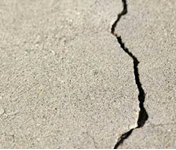
\includegraphics[width=0.5\linewidth]{img1}
    \end{minipage}
    %\end{minipage}
    \\ \hline
%---- dong 2
  Сеть трещин
    %\end{minipage}
    & 
    %\begin{minipage}{5cm}
      \begin{itemize}
        \item 	тип дефекта покрытия, который развивается из горизонтальных трещин и вертикальных трещин. Этот дефект обычно появляется на больших участках бетонной поверхности.
      \end{itemize}
			&
			 \begin{minipage}{.3\textwidth}
			\centering
      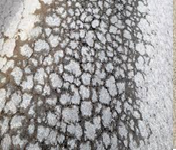
\includegraphics[width=0.5\linewidth]{img2}
    \end{minipage}
    %\end{minipage}
    \\ \hline
	%---- dong thu 3
	  Выбоина
    %\end{minipage}
    & 
    %\begin{minipage}{5cm}
      \begin{itemize}
        \item 	это расположение дорожной поверхности, которая подвергается воздействию нескольких слоев абразивного материала.

      \end{itemize}
			&
			 \begin{minipage}{.3\textwidth}
			\centering
      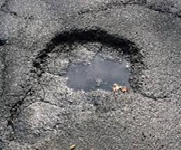
\includegraphics[width=0.5\linewidth]{img3}
    \end{minipage}
    %\end{minipage}
    \\ \hline
			%---- dong thu 4
	  Сдвиги, волны
    %\end{minipage}
    & 
    %\begin{minipage}{5cm}
\begin{itemize}
	\item  неровности в виде чередующихся поперечных выступов и впадин с пологими краями, вызванные смещением верхних слоев дорожных одежд капитального и облегченного типа.
\end{itemize}

			&
			 \begin{minipage}{.3\textwidth}
			\centering
      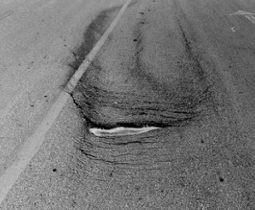
\includegraphics[width=0.5\linewidth]{pic56}
    \end{minipage}
    %\end{minipage}
    \\ \hline
					%---- dong thu 5
	  Гребенки
    %\end{minipage}
    & 
    %\begin{minipage}{5cm}

\begin{itemize}
	\item  неровности в виде чередующихся правильных и четко выраженных поперечных выступов и впадин на покрытиях переходного типа.
\end{itemize}

			&
			 \begin{minipage}{.3\textwidth}
			\centering
      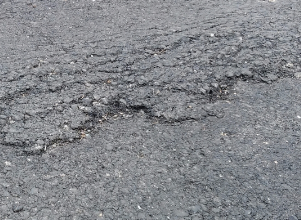
\includegraphics[width=0.5\linewidth]{pic57}
    \end{minipage}
    %\end{minipage}
    \\ \hline
						%---- dong thu 6
	  Колея
    %\end{minipage}
    & 
    %\begin{minipage}{5cm}

\begin{itemize}
	\item  деформация покрытия с образованием углублений по полосам наката с гребнями или без гребней выпора.
\end{itemize}

			&
			 \begin{minipage}{.3\textwidth}
			\centering
      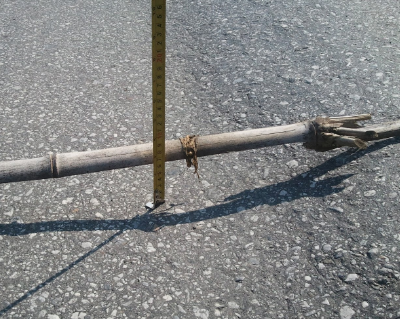
\includegraphics[width=0.5\linewidth]{pic58}
    \end{minipage}
    %\end{minipage}
    \\ \hline
  \end{tabular}
  \caption{Описание дефектов дорожного покрытия}\label{tab1}
\end{table}

%-------------1.2.2-------------%
\subsection{Методы извлечения признаков дефектов дорожного покрытия}
Изображения и видео - ввод данных системы обнаружения и классификации дефектов дорожного покрытия. Эти данные предварительно обрабатываются, из них извлекаются признаки, затем формируются векторы признаков. Однако в реальности исходные данные известны с точностью до уровня шума. Фактические условия окружающей среды (свет, дорожные характеристики и т.д.) оказывают большое влияние на сбор данных. Подход к решению проблемы заключается в выборе алгоритмов, настройке их параметров, комбинаций методов обработки. Поэтому системы привлекают внимание многих ученых и исследовательских центров по всему миру.

В данной работе мы сосредоточились на изучении, таких признаков извлеченных из изображений, как признаки контуров, признаки формы дефектов дорожного покрытия, а затем применяем соответствующие алгоритмы машинного обучения для их классификации и сокращения времени вычисления и затрат памяти.

Дефекты покрытия являются объектами входных изображений системы выявления и классификации дефектов. Извлечение признаков объекта является важным шагом в анализе данных. Для этого в работе предполагается использование методов обработки изображений для анализа и преобразования информации изображения в векторы признаков для обнаружения и классификации дефектов дорожного покрытия. Метод с использованием вейвлет-преобразования \cite{h61}, метод выборки \cite{h62}, мера анизотропии \cite{h63}, метод на основе алгоритмов нечеткой логики \cite{h64}, метод выборочной экстракции \cite{h65} для решения проблемы извлечения признаков дефектов дорожного покрытия на основе данных избражений и видео.

В \cite{h108} представлен метод извлечения с использованием вейвелет-преобразования. Использование вейвлет-преобразования позволяет проводить анализ дефектов трещин на дорожном покрытии. На рисунке \ref{pic1} описан процесс разложения изображения на основе вейвлет-преобразования, где L и H соответственно фильтры.
\begin{figure}[ht!]
\centering
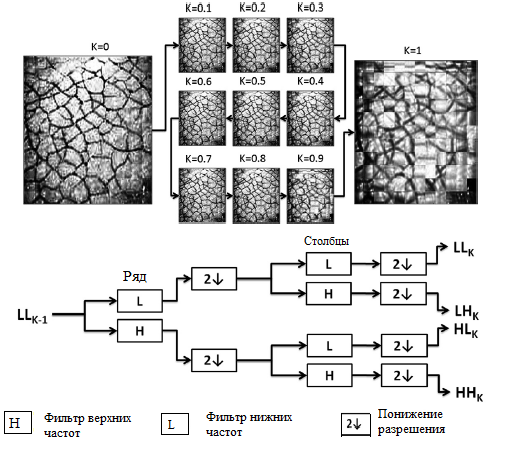
\includegraphics[width=0.8\linewidth]{pic1}
\caption{Метод извлечения признаков дефектов дорожного покрытия методом Wavelet -Random transform \cite{h108}}
	\label{pic1}
	\end{figure}
	
Анализ формы очень важен для выделения дефектных пикселей с соседними пикселями. В исследовании использовался метод извлечения линейных признаков глубоких трещин на дорожном покрытии - линейных износов \cite{h102}. Термин <<линейный изноз>> впервые был предложен в работе \cite{20wl}. На рис.\ref{pic2} описывается использование двумерного дискретного вейвлет-преобразования и фильтров на основе методов математической морфологии.
\begin{figure}[ht!]
\centering
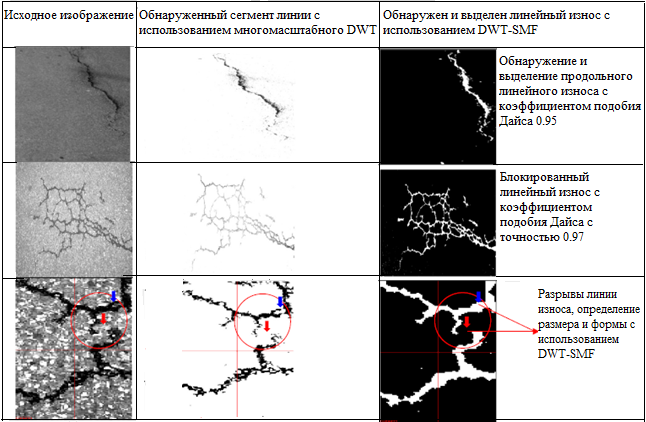
\includegraphics[width=0.8\linewidth]{pic2}
\caption{Метод извлечения признаков на основе DWT--SMF (discrete wavelet transform -- successive morphologic transform filtering) \cite{h102}}
	\label{pic2}
	\end{figure}

Метод на основе нечеткой логики применяется для извлечения признаков дефектов дорожного покрытия - глубоких трещин. На рисунке (\ref{pic3}a) показано начальное изображение, на рисунке (\ref{pic3}b) показаны результаты сегментации. Рисунки (\ref{pic3}c, d) отображают результаты извлечения конкретных краев.
\begin{figure}[ht!]
\centering
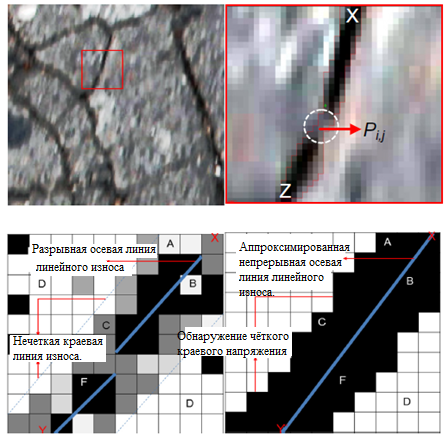
\includegraphics[width=0.6\linewidth]{pic3}
\caption{Результаты извлечения признаков «нечётких» дефектов дорожного покрытия \cite{h102}}
	\label{pic3}
	\end{figure}
	
В работах \cite{h79, h80, h81, h82} применены методы обработки изображений для удаления фоновых изображений, но результаты по-прежнему содержат области без дефектов. Методы машинного обучения используются для отделения дефектов дорожного покрытия от этих областей. В таких исследованиях использовались различные признаки: толщины, площади и пластичности поверхности являются признаками, которые широко используются для выявления интересующих областей.
	
Однако на практике извлечение признаков для обработки является интуитивным и основано на наблюдениях человека. Для создания максимально информативных признаков необходимо уметь оценивать важность их отдельных компонент.
%------------1.2.3-------------%
\subsection{Методы машинного обучения в обнаружении и классификации дефектов дорожного покрытия}
Методы машинного обучения были разработаны и широко применяются для решения задачи обнаружения и классификации дефектов дорожного покрытия. Методы машинного обучения оценивались на основе критериев: времени выполнения, стабильности системы для несбалансированных данных (например, наличие редких типов дефектов), стабильности системы для косвенных факторов (шум, свет и т.д.), способности интерпретировать результаты и ясности процедур (т.е. минимум параметров для настройки).
\begin{figure}[ht!]
\centering
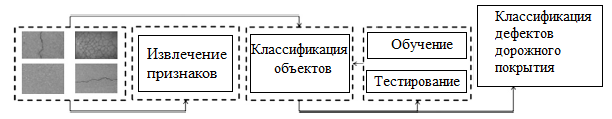
\includegraphics[width=0.8\linewidth]{pic4}
\caption{Общая структура системы обнаружения и классификации дефектов дорожного покрытия.}
	\label{pic4}
	\end{figure}
	
	Методы и алгоритмы машинного обучения были успешно применены и разработаны при автоматическом обнаружении и классификации дефектов дорожного покрытия и имеют общую структуру, как показано на рисунке \ref{pic4}. Эти алгоритмы перечислены в таблице \ref{tab2}. Рассмотрим их более подробно.
	
	 \begin{table}[h!]%
\centering
\caption{Анализ алгоритмов машинного обучения (****: Лучший, *: Худший).}
\label{tab2}
  \begin{tabular}{|c|c|c|c|c|}
    \hline
     \multirow {3}{*}                 &{Деревья} & {Нейронные} & {Наивный}  & {}МОВ\\
		                                  & {решений}& {сети}      & {байесовский} &{}\\
																		 	&&&{классификатор}&\\
    \hline
\multirow {2}{*}{Тип машинного}&{Обучение} 	     &{Обучение} 	&{Обучение}    &{Обучение} \\
                {обучения}    & {без учителя}    &{с учителем} &{с учителем} &{с учителем}\\
\hline 
Точность                    &**   &***  &*  &****\\
\hline 
\multirow {2}{*}{Скорость}  &{***}  &{*}    &{****} &{*}\\
                 {обучения} & {}    &{}     &{}     &{}\\
\hline 
\multirow {2}{*}{Классификация}      &{****}	&{****}	&{****}	&{****} \\
                {скорости }          & {}    &{}     &{}     &{}\\
\hline 
\multirow {2}{*}{Среднеквадратическое}  &{**}   &{**}	  &{***}	&{**} \\
                {отклонение с шумом}    & {}    &{}     &{}     &{}\\
\hline
\multirow {2}{*}{Улучшение процесса}    &{**} &{***} & {****} & {**}\\
\multirow {1}{*}{обучения}            & {}    &{}     &{}     &{}\\
\hline
  \end{tabular}
\end{table}%\vspace{10mm}

\textbf{Дерево решений}. Деревом решений является древовидная структура, в которой каждый узел представляет соответствующий признак. Каждая ветвь представляет результат теста. Узлы обозначают классы или распределения классов \cite{h83}. Чтобы классифицировать неизвестный образец, значения признака этого образца меняются на дерево решений.

Дерево решений можно трансформировать в набор правил классификации \cite{h84, h85}. Математическая основа дерева решений - это <<жадный алгоритм>>, который построил реверсивное дерево решений сверху вниз. Преимущество этого метода заключается в том, что его легко реализовать, легко понять и легко выполнить.

\textbf{Нейронные сети}. Искусственные нейронные сети (ANN) организованы в слои, каждый из которых состоит из взаимосвязанных узлов, содержащих функцию активации\cite{h86}. ANN создают систему обработки информации, которая имитирует нейронную систему мозга человека. Обработка информации в нервной системе состоит из двух частей: обработка входного сигнала и вывод выходного сигнала. Эти два класса взаимодействуют друг с другом через один или несколько скрытых слоев. Элементы в разных классах взвешены. Весовое значение может быть исправлено путем обучения правилам через входные значения, которые  используются \cite{h87, h88}. 

Преимущество этого подхода состоит в том, что он является мощным методом моделирования, который был успешно применен для классификации дефектов дорожного покрытия \cite{h92, h93}.

\textbf{Наивный Байесовский классификатор}. Байесовский метод классификации основан на статистических методах. Этот метод может прогнозировать вероятности классов в наборе данных на основе этой вероятности, которые могут быть помещены в отдельные классы \cite{h89, h90}. Байесовская сеть представляет собой график на графике, который позволяет выражать отношения между признаками.

\textbf{Метод опорных векторов - МОВ} \cite{h91} был впервые предложен Вапником в 1960 году для классификации данных и привлекл большой интерес. МОВ - очень общий метод, который может быть применен к широкому спектру проблем идентификации дефектов дорожного покрытия и классификации \cite{h94}. Целью метода МОВ является создание модели из набора моделей, которые имеют возможность прогнозировать классы для объектов.

Преимущества МОВ: очень эффективен при решении больших размерных данных (анализ экспрессии генов, белков, данных клеток), МОВ позволяет решать проблему переобучения очень хорошо (при наличии шума в данных или когда данных для обучения слишком мало), является быстрым методом классификации, обладает хорошей совокупной производительностью и высокой вычислительной эффективностью.

Существуют различные методы обнаружения дефектов дорожного покрытия на основе характеристик цвета и яркости \cite{h66}, анализа пороговых значений \cite{h67}, признаков структурных характеристик изображений \cite{h68}. Имеется много разных подходов для обнаружения дефектов дорожного покрытия. Один из самых распространенных подходов осуществляется путем анализа гистограмм с использованием искусственных нейронных сетей (ИНС). 

В работе \cite{h69} авторы для классификации сегментов дорожных изображений и трещин предлагают методику, основанную на нейронной сети. Проводится анализ гистограмм изображений. Признаки передаются в нейронную сеть для последующей классификации. После того как изображения классифицируются на наличие трещин, участки, не имеющие трещин, после их сегментации передаются в другую нейронную сеть для классификации типа трещин. Модели на основе теории графов широко используется для сегментации, что отражено, например, в работе \cite{h70}. В работе \cite{h71} авторы предложили объединить методы математической морфологии и преобразования Фурье для создания признаков, которые были классифицированы на основе классификатора AdaBoost \cite{h72}.

В статье \cite{h73} авторы обсудили проблемы автоматического анализа видео, чтобы следить за состоянием дорожного покрытия в лабораторных условиях и показали, что использование компьютерного зрения для решения задач анализа изображений позволяет сократить время внедрения и дает более высокую точность.

Был предложен способ обнаружения поверхностных контуров, который не зависит от теней, освещения и неровностей. Этот метод основан на обработке изображений с использованием локальных особенностей градиента, линейного предсказания \cite{h74} и анализа градиентов изображений \cite{h75}. 

В работе \cite{h76} Лемперт, Сидоров и Жуков представили подход к проблеме определения приоритетов работ по ремонту дорожного покрытия с ограниченными ресурсами, который использует комбинацию методов распознавания и классификации дефектов на основе статистического анализа и машинного обучения с оригинальными методами для решения задачи оптимизации и определения приоритетов работ (оптическая – геометрическая аналогия).

Авторы в работах \cite{h77, h78} предложили два новых метода для регистрации дефектов дорожного покрытия. Подходы основаны на видеосистеме, представляющей собой автомобиль, на котором установлен комплекс для сбора и анализа данных дорожной поверхности. Используется метод сегментации изображений, затем дефекты классифицируются с помощью определенного классификатора. 

В статье \cite{ h103} автор создал систему, состоящую из трех основных частей (рис. \ref{pic5}): предварительная обработка и улучшение качества цифровых изображений, извлечение геометрических объектов в каждой области изображения, обнаружение и идентификация дефектов на основе вейвлет-преобразований для изображений с низким разрешением, использование срединных фильтров для получения пороговых значений, использование морфологических фильтров для признаков формы, использование случайных величин для классификации типов дефектов дорожного покрытия.   
\begin{figure}[ht!]
\centering
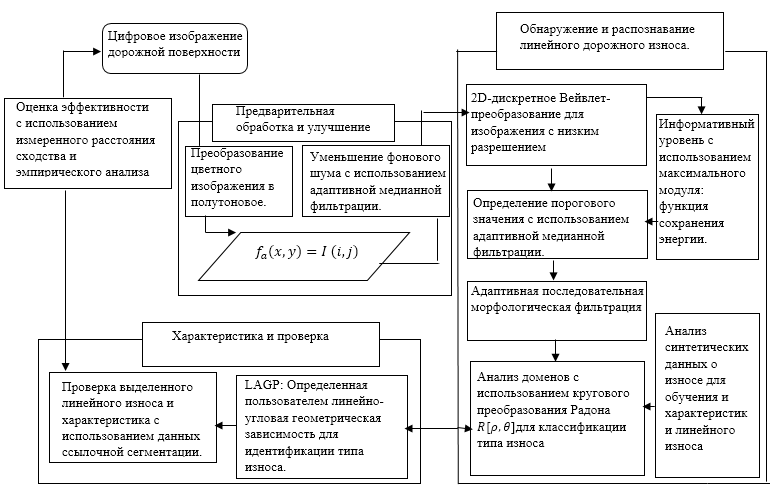
\includegraphics[width=0.8\linewidth]{pic5}
\caption{Блок-схема подхода к обнаружению и идентификации линейных дефектов в дорожных покрытиях на цифровых изображениях \cite{h103}.}
	\label{pic5}
	\end{figure}

В \cite{h110} подход машинного обучения использовался для обнаружения и классификации дефектов выборок на видео (рис.\ref{pic6}). Изображения сегментируются в регионы, извлекают формы и текстурные признаки для обнаружения выбоин. Геометрические признаки количественно определяются эллиптической регрессией.
\begin{figure}[ht!]
\centering
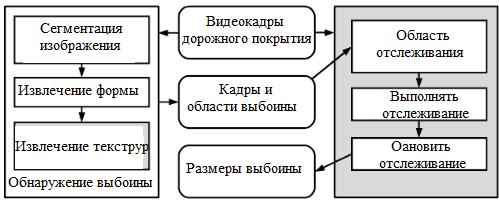
\includegraphics[width=0.8\linewidth]{pic6}
\caption{Описание основных частей системы обнаружения дефектов выбоин на видео \cite{h110}.}
	\label{pic6}
	\end{figure}

В \cite{h104} представлена система автоматического обнаружения и классификации дефектов дорожного покрытия на основе комбинации вейвлет-преобразования и нейронной сети (рис.\ref{pic7}). Система состоит из трех основных частей: первая часть - обработка и сохранение входного изображения, вторая часть - извлечение признаков на основе Фурье преобразования и балансе гистограммы, классификация дефектов с использованием нейронных сетей. Третья часть - отображение результатов классификации.
\begin{figure}[ht!]
\centering
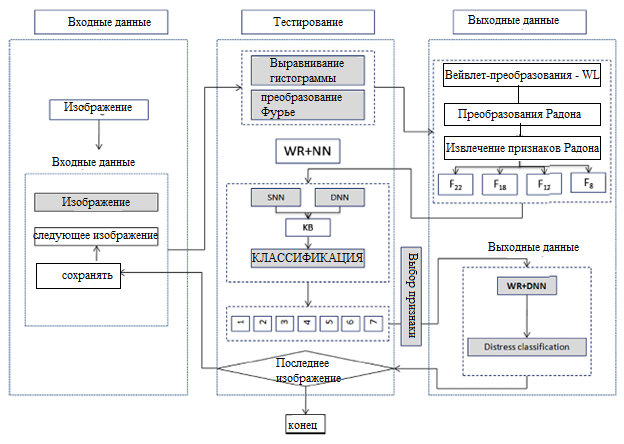
\includegraphics[width=0.8\linewidth]{pic7}
\caption{Система автоматически классифицирует и обнаруживает глубокие трещины с использованием динамических нейронных сетей \cite{h104}.}
	\label{pic7}
	\end{figure}
%-----------1.2.4===============%
\subsection{Программы обнаружения и классификации дефектов дорожного покрытия на основе методов машинного обучения}
В течение многих лет были разработаны программы автоматического обнаружения и классификации дефектов дорожного покрытия. Эти данные собираются и сохраняются \cite{h95, h96}. Обзор доступных источников продемонстировал недостатки существующих систем в первую очередь связанные с их высокой стоимостью.

В последние годы получили широкое распространение цифровые системы. Такие системы обрабатывают видеопоток достаточно высокого разрешения. На основании этого можно сделать вывод о необходмости привлечения использования алгоритмов машинного обучения.

Существует множество систем для автоматического обнаружения трещин с использованием линейных сканеров. Предлагаемые системы проводят классификацию согласно ширине дефекта.

В 1999 году Организация научных и промышленных исследований Австралийского содружества (CSIRO) первой разработала систему автоматического обнаружения дефектов трещин - RoadCrack \cite{h18}. 

Платформа ARAN \cite{h97} широко используется в Соединенных Штатах для автоматического анализа дорожных покрытий. Эта система проводит сбор данных, где изображения оцениваются с помощью автоматизированного программного обеспечения для обнаружения трещин - WiseCrax \cite{h19}. Также популярна программа автоматического обнаружения транспортных средств WayLink Digital Highway Data Vehicle \cite{h98}.

В европейских странах система PAVUE \cite{h99} нашла применение в Нидерландах и Финляндии. Система оснащена двумя видеокамерами для сбора данных и настройки компьютера, которые объединяют алгоритмы машинного обучения.

Система использует высокоскоростную технологию обработки, объединяющая устройство для сбора и хранения данных (рис.\ref{pic8}). Это устройство включает в себя цифровые камеры, ультразвуковые и лазерные технологии для сбора структурных дефектов на дороге.
\begin{figure}[ht!]
\centering
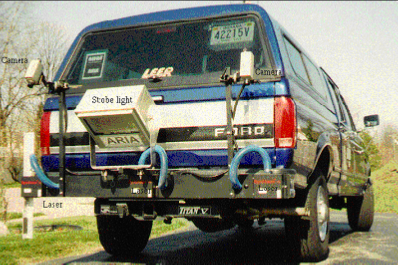
\includegraphics[width=0.5\linewidth]{pic8}
\caption{Устройства сбора изображений дорожного покрытия \cite{h109}.}
	\label{pic8}
	\end{figure}
	
Система LRIS состоит из камер высокого разрешения и лазерных источников (рис. \ref{pic9}). Эти камеры установлены на оборудованных для сбора данных автомобилях для и классификации дефектов дорожного покрытия. Данные считываются в автономном режиме с помощью автоматической программы обнаружения трещин \cite{h16}. Преимуществами системы являются быстрота и безопасность.
\begin{figure}[ht!]
\centering
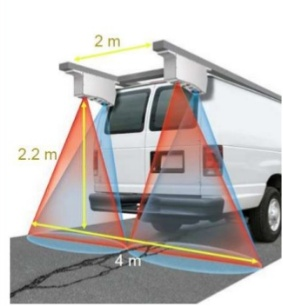
\includegraphics[width=0.5\linewidth]{pic9}
\caption{Система IRIS \cite{h16}.}
	\label{pic9}
	\end{figure}
	
Система GIE LaserVISION \cite{h100} является ярким примером использования лазерной технологии для автоматического обнаружения и классификации дефектов дорожного покрытия. Система использует четыре лазерных датчика и обеспечивает 3D-вычисления для улучшения расчета дефектов в 3D. Однако, разрешение системы низкое, и работает только с горизонтальными трещинами. Основные проблемы обработки видеоданных подобными системами связаны с освещением, углом регистрации изображений дорожного полотна и др. Чтобы уменьшить влияние этих факторов, система StereoVision \cite{h101, h106, h107} использует 3D-технологию для повышения производительности системы.
%%----------1.2.5----------------------%
\subsection{Комбинация метода Марковского случайного поля с методом разреза на графах для сегментации изображений}
Между соседними пикселями в изображениях всегда существует определенная связь. Поэтому статистические модели хорошо подходят для представления этих взаимодействий. В последнее время исследования по решению проблемы сегментации изображений были сфокусированы на модели Марковского случайного поля (MRF) \cite{h111, h112}. В этом разделе анализируется подход к решению проблемы сегментации изображения на основе модели MRF.

Марковское случайное поле можно рассматривать как частный случай случайного поля \cite{h113}, в котором состояние случайной величины зависит только от состояния «смежных» случайных величин. Преимуществами модели MRF являются следующие: В основе MRF лежит хорошо проработанная теория; алгоритм не требует предположения независимости наблюдаемых переменных. Кроме того, использование произвольных факторов позволяет описать различные признаки определяемых объектов, что снижает требования к полноте и объему обучающей выборки.

Алгоритм случайных полей рассматривается как инструмент структурного анализа. Сочетание спектральных и структурных признаков приводит к лучшему анализу изображения. На основе структуры можно определить вероятность появления объекта находящегося в определеной связи с соседними пикселями.

\textbf{a) Марковские случайные поля в сегментации изображения}

Модели MRF часто используются для решения проблем сегментации изображений. В \cite{h114} автор предоставил эффективный метод сегментации изображений без учителя. Использовался иерархический генетический алгоритм для решения сложной вычислительной задачи MRF с использованием моделей. 

В \cite{h115} также был предложен подход к сегментации изображения на основе MRF и разделения исходного изображения на независимые области в виде смежных графов. Для этого были определены надежные признаки и их интеграция в энергетическую функцию, которая управляет процесс. В \cite{h116} предлагается подход, основанный на алгоритме сегментации неэкранированного изображения и модели MRF. Этот метод решения проблем шума и текстуры изображения. Количество классов и параметров модели задано в соответствии с каждым стандартным сегментом изображения \cite{h117}. Результаты демонстрируют улучшение эффективности и надежности.

В \cite{h118} автор представляет два метода сегментации изображений: с учителем и без учителя. Предлагаемый алгоритм может обеспечить максимальный метод с учителем сегментации изображения. В сегментации изображения без учителя была предложена схема параметрической оценки для непосредственного вычисления параметров модели из данного изображения.

Многие другие исследования использовали модель MRF для решения проблем сегментации изображений \cite{h119}. В \cite{h120} предложен алгоритм для сегментирования изображений на основе текстуры изображений с использованием алгоритма вейвлет и MRF. Результаты представлены в \cite{h121, h122} с использованием модели MRF для сегментирования изображений дистанционного зондирования для получения точных и эффективных результатов.

\textbf{b)	Объединение метода разреза на графах с методом MRF}

Метод MRF используется в качестве модели для решения пометок при обработке изображений. Этот метод широко используется для моделирования проблем, таких как восстановление изображений, сегментация изображения, структурный анализ и т. д. Метод разреза на графах считается эффективным способом решения проблемы минимизации энергии в области машинного обучения. Было проведено много исследований с использованием метода разреза на графах для решения вычислительных задач MAP-MRF.

Бойков \cite{h123} предложил новый метод решения проблемы MAP-MRF с использованием алгоритма разреза на графах. На граф был применен метод минимального потока с минимальным разрезом, который продемонстрировал важность метода разрезов графов . Этот алгоритм может решать энергетические функции с элементами MAP-MRF.

Коли и Торр \cite{h124} представили абсолютно новый динамический алгоритм для проблемы <<st-минимального разреза>>, который может быть использован для быстрого поиска решений MAP для некоторых динамически изменяющихся MRF. Этот метод является общим и находит точное решение для всех динамических задач, которые могут быть сформулированы как энергетические функции двоичных переменных. Результаты показали, что их алгоритм существенно быстрее, чем самый известный статический алгоритм.

Алгоритм разреза графов широко используется в области компьютерного зрения. Этот алгоритм используется для сегментации медицинских изображений или сегментации видео \cite{h125}. Авторы Бойков и Джолли \cite{h126} первыми предложили и протестировали алгоритм двоичного разреза графов для сегментации объектов.

В работе \cite{h127} существует несколько алгоритмов для тестирования и применения в сегментации двоичного изображения. Бойков и Функалед предложили методы извлечения признаков объектов с помощью разрезов на графах \cite{h128}. Этот метод может быть применен к интересующей предметной области изображения. Алгоритм <<минимального разреза -- максимального потока>> был протестирован в сегментации 2D и 3D-изображений. Результаты демонстрируют эффективность метода и применения алгоритма разрезов на графах в сегменте изображения.

%%----------1.2.6----------------------%
\section{Алгоритм случайного леса в задаче классификации данных}
Алгоритм <<случайный лес>> - это классификатор объектов. Этот метод разработан Лео Брейманом в Калифорнийском университете в Беркли \cite{h129}. Брейман также является соавтором методологии классификации и регрессии (CART), которая считается одной из 10 лучших классических методов интеллектуального анализа данных. Случайный лес построен на трех основных компонентах: CART, комбинированной модели и синтезе бутстрепа.
Процесс изучения случайный лес предполагает использование случайных входных значений или комбинаций этих значений в каждом узле для построения дерева решений. Алгоритм случайный лес имеет некоторые сильные атрибуты, такие как: 

\begin{itemize}
	\item Его точность похожа на Adaboost, в некоторых случаях превосходит его. 
\item Этот алгоритм правильно решается с данными, которые имеют большой шум. 
\item Время работы алгоритма быстрее, чем Бэггинг или Бустинг. 
\item Легко реализуется параллельно.
\end{itemize}

Однако для достижения вышеуказанных свойств время выполнения алгоритма достаточно длительное и необходимо использовать много ресурсов системы. Таким образом, можно сказать, что алгоритм случайный лес является хорошим методом классификации в виду следующих причин: в алгоритме случайный лес дисперсия минимизируется в результате синтеза случайного леса во многих процессах обучения; выбор случайных значений на каждом шаге в случайном лесе уменьшит корреляцию между изучаемыми в синтезе результатов.

Кроме того, общая ошибка подкласса леса зависит от ошибки отдельных деревьев в лесу, а также от каждой взаимосвязи между деревьями.

\textbf{Оценить ошибку OOB алгоритма случайный лес.} Образец был составлен из учебного набора, было подсчитано, что около $1/3$ элементов не были включены в образец. Это означает, что изучались только около $2/3$ элементов, участвующих в расчете $1/3$ , получены данные об общей сумме. Данные об общей сумме используются для оценки ошибки результатов и оценки важности каждого признака. Реализация вычисления для определения важных атрибутов в алгоритме случайного леса такая же, как и использование OOB для вычисления ошибок в алгоритме случайного леса. 

%--------1.3---------------------%
\section{Анализ подхода к использованию машинного обучения при обнаружении пузырьков}
В этом разделе представлены работы по исследованию и применению методов машинного обучения в проблеме обнаружения пузырьков. Кроме того, были успешно построены оценки программ, они демонстрируют свое приложение на практике. Учитывалась возможность применять Wavelet Transform в пузырьках как функцию.
%%-------1.3.1------------------%
\subsection{Методы обнаружения пузырьков}
Во время анализа изображения пузырьков методы машинного обучения включают в себя два основных процесса, которые представляют собой процесс сегментации изображения для обнаружения местоположений пузырьков и идентификации их формы (одиночный, перекрывающий, частично стирающийся), а затем процесс извлечения признаков, таких как радиус, диаметр, площадь, координаты центра и т.д. от экспериментальных данных.

В работе \cite{h1bb} представлен метод идентификации изображений пузырьков на основе алгоритма сверточных нейронных сетей \cite{h6bb}. Нейронные сети способны определять перекрывающиеся, размытые и несферические пузырьковые изображения. Моделируются реалистичные пузырьковые изображения из экспериментальных данных для создания синтетических изображений, необходимых для обучения нейронных сетей. Это повысило точность распознавания изображений пузырьков, уменьшило количество выбросов, снизило время работы. Предложен метод обнаружения пузырьков прозрачных объектов в жидкости. Авторы сформулировали проблему обнаружения концентрических круговых устройств. Генерация гипотезы основана на выборке из подключенных компонентов ответов подавления ориентированных хребтовых фильтров и оценки параметров концентрических круговых устройств. Предложен способ обнаружения пузырьков, который показал удовлетворительную производительность в промышленном применении, требующий оценки объема газа в суспензии целлюлозы при достижении средней относительной погрешности \cite{h2bb}.

В работе \cite{h3bb} описывается новый признак, который был разработан для автоматического распознавания нефти из других круглых объектов, найденных на изображениях.

В статье \cite{h4bb} предложена система измерения пузырьков, в которой используется метод обнаружения на основе шаблонов. Предлагаемый подход говорит о слабой эффективности традиционных методов для обнаружения пузырьков. В предлагаемом подходе используются шаблоны для повышения надежности и масштабирования изображения для обнаружения пузырьков независимо от их размера.

В статье \cite{h5bb} авторы предоставили метод сегметации пузырьков потока газа $/$ жидкости двухфазного потока на основе оператора Canny \cite{h7bb} и гауссовского гладкого фильтра \cite{h8bb} многопоточного высокоскоростного видеоанализа для сохранения краев и устранения шума. Этот метод очень эффективен для анализа и распознавания многопоточного потока пузырьков.

В статье \cite{h9bb} описана новая полуавтоматическая методика онлайн-оценки диаметров пузырьков нефти и воздушных пузырьков. Изображения данных были предварительно обработаны, чтобы найти края сегментов областей, представляющих интерес. Алгоритм преобразования Хафа \cite{h10bb} используется для восстановления контуров воздушных пузырьков и  пузырьков нефти. Этот метод позволил сократить общее время обработки измерения пузырьков в другой системе.

В работе \cite{h11bb} представлена проблема важности захвата изображений и сегментации, включая гетерогенную прозрачность движущихся объектов интереса и фона, размытие, перекрытие и артефакты на основе метода преобразования Хафа, который был реализован и протестирован. В статье также сделан вывод, что оценка распределения размеров воздушных пузырьков при механическом перемешивании проводилась более эффективным и менее трудоемким способом, чем другие полуавтоматические или ручные методы. 

В \cite{h12bb} предлагается метод перекрывающегося пузырькового расщепления. Во-первых, получается выпуклая оболочка перекрывающегося объекта. Во-вторых, пересечение основано на контуре объекта в каждом пузырьке после повторного поиска, а затем точечные пары перекрывающихся пузырьков получаются путем сопоставления на основе средней оси (МА). Наконец, точность вычисления области пересечения пузырьков обеспечивается путем построения эллипса на основе значений точек пересечения при использовании минимальной среднеквадратической ошибке (MMSE) с ограничениями пересечения.
%---------------1.3.2 ---------------%
\subsection{Программы обнаружения пузырьков}
В настоящее время существует множество проектов, разработавших системы обнаружения пузырьков на основе результатов исследований, например: использование двухфазных пузырьковых потоков во многих технологических и энергетических процессах в качестве технологических, химических и ядерных реакторов. Это объясняет большой интерес к экспериментальным и численным исследованиям таких потоков за последние несколько десятилетий. Использование оптической диагностики для анализа пузырьковых потоков позволяет исследователям получать мгновенные поля скоростей и распределение газовой фазы с высоким пространственным разрешением. Эта работа представляет собой метод идентификации изображений пузырьков, основанный на современной технологии глубокого обучения, называемой сверточными нейронными сетями (CNN). Система обнаружения пузырьков воды \cite{h1bb} основана на новой SIFT \cite{h13bb} и гистограмме метода ориентированных градиентов (HoG) \cite{h14bb}.
\begin{figure}[ht!]
\centering
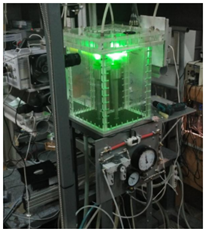
\includegraphics[width=0.3\linewidth]{pic10}
\caption{Система обнаружения пузырьков воды на основе метода CNN.}
	\label{pic10}
	\end{figure}

Нейронные сети способны определять перекрывающиеся, размытые и несферические изображения пузырьков. Система может повысить точность распознавания изображений пузырьков, уменьшить количество выбросов, сократить время обработки данных и значительно уменьшить количество настроек для идентификации объекта по сравнению со стандартными методами распознавания, разработанными ранее (рис. \ref{pic10}). Кроме того, использование графических процессоров ускоряет процесс обучения CNN, владеющего современными адаптивными методами оптимизации субградиента.

\begin{figure}[ht!]
\centering
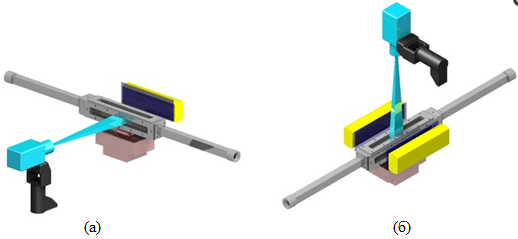
\includegraphics[width=0.5\linewidth]{pic11}
\caption{Система обнаружения пузырьков на основе методов анализа изображений.}
	\label{pic11}
	\end{figure}
	
В этой работе \cite{h15bb} было предложено использовать машинное зрение в процессе массового распознавания пузырьков, что подтверждает валидацию моделей кипения, связанных с динамикой пузырьков, а также частоту зарождения, плотность активного слоя и размер пузырьков (рис. \ref{pic11}). Два предложенных алгоритма предназначены для получения стандартных изображений пузырьков, наблюдающихся при барботаже в кипятильных устройствах общего назначения.

\begin{figure}[ht!]
\centering
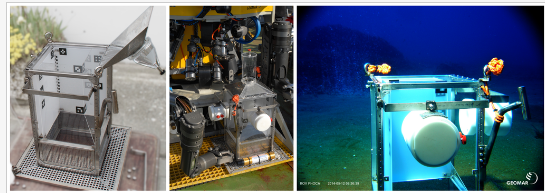
\includegraphics[width=0.7\linewidth]{pic12}
\caption{Система обнаружения пузырьков на основе технологии 3D-анализа изображений.}
	\label{pic12}
	\end{figure}
	
В этой статье \cite{h16bb} авторы представляют  широкую базовую стереопанельную камеру с широким разрешением, которая преодолевает многие ограничения, поскольку она наблюдает пузыри в двух ортогональных направлениях, используя калибровочные камеры. Помимо описания установки и аппаратного обеспечения системы, в ходе исследования обсуждаются соответствующие калибровки, а также различные автоматические этапы обработки деблокирования, обнаружения, отслеживания и 3D-фитинга, которые имеют решающее значение для получения трехмерной эллипсоидальной формы и повышения скорости каждого пузыря. Полученные значения для одиночных пузырьков могут быть агрегированы в статистические распределения размеров пузырьков или потоки для экстраполяции на основе моделей диффузии и растворения и крупномасштабных акустических съемках. Результаты исследования демонстрируют и дают оценку широкой базовой модели стереоизмерений с использованием контролируемой тестовой установки с информацией о входных данных.

%---------1.3.3 -----------------------------
\subsection{Признак вейвлет-преобразования при обнаружении объектов}
Научное направление сконцентрировано на анализе и применении, связанное с так называемым вейвлетами. Вейвлеты широко применяются  при решении ряда задач, таких как: сжатие и обработка изображений, распознавание образов, обработка и синтез сигналов и т.д. Вейвлеты могут быть ортогональными, полуортогональными и биортогональными. Вейвлет-коэффициенты определяются интегральным преобразованием сигнала \cite{1wl}.

Вейвлет-преобразование похоже на преобразование Фурье, но с совершенно иной оценочной функцией. Основное различие лежит в следующем: вейвлет-преобразование использует функции, локализованные как в реальном, так и в Фурье-пространстве. В общем, вейвлет-преобразование (wavelet transform) является инструментом, разбивающим данные, функции, операторы на составляющие с разными частотами, каждая из которых затем изучается с разрешением, подходящим масштабу \cite{2wl}.

Вейвлет-преобразование разделяется на непрерывное вейвлет-преобразование (НВП) \cite{3wl} и дискретное вейвлет-преобразование (ДВП) \cite{1wl}.

В машинном зрении преобразование Вавелет широко используется в качестве метода обработки изображений для обнаружения и классификации объектов.

В работе \cite{5wl} вейвлеты использовались для анализа изображений и использовались во многих приложениях дистанционного зондирования, таких как слияние изображений с высоким спектральным разрешением с изображениями с высоким пространственным разрешением, анализ текстур и классификация \cite{6wl}, удаление шума из радарных изображений.

Вейвлет-преобразование эффективно используется для удавления шумов с изображений. Изображение претерпевает вейвлет-преобразование, фильтрацию и обратное вейвлет-преобразование (рис.\ref{pic13}) \cite{8wl}.
\begin{figure}[ht!]
\centering
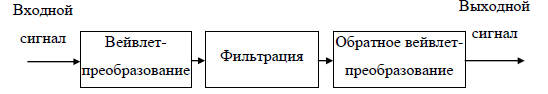
\includegraphics[width=0.8\linewidth]{pic13}
\caption{Использование вейвлет-преобразования при фильтрации шума.}
	\label{pic13}
	\end{figure}
В работе \cite{9wl} вейвлет-преобразование использовалось для классификации сигнала ЭЭГ с интеграцией экспертной модели.

В статье \cite{10wl} вейвлет-преобразование применялось для классификации заземления. Реализация дискретного преобразования вейвлета (ДВП) в качестве метода обработки изображений дает значения преобразования, называемые коэффициентом вейвлет-коэффициента. Задачи представляют собой определение объекта для обнаружения и классификации для  определения коэффициента.

Подход к извлечению признаков, основанный на вейвлет-преобразовании, представляет собой вычисление распределения коэффициентов по выбранному признаку вейвлета. Общей методикой, используемой для выделения признаков ДВП-коэффициента, является использование нейронных сетей \cite{11wl, 12wl, 13wl}.

Алгоритм преобразования вейвлетов представлен в работе \cite{14wl}. Вейвлет-преобразование используется с определенной шкалой разложенного сигнала измерения расхода. Из детального коэффициента вычисляется адаптивный порог и проверяется на подробные коэффициенты. Газовые пузырьки обнаруживаются, если подробные коэффициенты превышают порог в конкретный момент времени.

%%==========1.4----------------------%
\section{Основные результаты и выводы по главе 1}

\begin{enumerate}
	\item В содержании главы 1 было рассмотрено машинное обучение, классификатор и применение машинного обучения на практике, комбинированные методами методы классификации данных. Рассматривались некоторые проблемы в оценке ошибки метода классификации методов машинного обучения.
	\item В первой главе были проанализированы методы обработки изображений в извлечении признаков для двух задач ОКДДП и ОКФП.
\item  В этой главе анализировался подход алгоритмов и методов машинного обучения в классификации данных. Были освещены следующие алгоритмы, методы:

\begin{itemize}
	 \item Дерево решений
   \item Нейронные сети 
   \item Наивный байесовский классификатор
   \item Метод опорных векторов – МОВ
\end{itemize}

\item Рассмотрена возможность использования алгоритма Марковского случайного поля в сочетании с методом разрезов на графах для построения карты дефектов дорожного покрытия и алгоритма случайного леса для классификации данных дефектов дорожного покрытия на изображениях и видео.
\item Рассмотрена возможность использования вейвлет-преобразования в качестве признака для обнаружения пузырьков на фотографиях.
\end{enumerate}
В этом исследовании реализована комбинация методов обработки изображений для данных процесса в условиях нормального освещения и большого шума. Реализованы методы и алгоритмы машинного обучения для решения основной задачи: извлечения признаков, обнаружения и классификации объектов в фотографиях и видео, обеспечена стабильность системы, получена хорошая производительность, обработка данных выполнялась быстро и точно.

Целью этой диссертации является разработка алгоритмов, методов машинного обучения для создания автоматизированной системы для извлечения признаков, обнаружения и классификации объектов в изображениях и видео. Для достижения указанных выше целей необходимо решить следующие задачи:

\begin{itemize}
	\item Создать и разработать методы обработки данных на изображениях и видео.
\item	Проанализировать и улучшить метод обнаружения объектов в соответствии со сменой света для построения карты дефектов дорожного покрытия, чтобы определить границу между объектом для пузырьков воздуха.
\item	Применить алгоритмы, методы обработки изображений для извлечения признаков объектов при наличии шума.
\item	Разработать и внедрить обнаружение и классификацию дефектов дорожного покрытия на основе методов, алгоритмов машинного обучения.
\item	Разработать и внедрить обнаружение и расчет диаметров баллона с использованием функции вейвлет-преобразования .
\item	Создать и оценить точность функций автоматической системы обнаружения, классификации дефектов дорожного покрытия и систем обнаружения воздушных пузырьков.

\end{itemize}

%%%%%%%%%%%%%%%%%%%%%%%  ГЛАВА 2 %%%%%%%%%%%%%%%%%%%%%%%%%%%%%%%%%%%%%%%%%
\chapter{Математические модели и численные методы для решения задачи классификации объектов на основе методов компьютерного зрения и машинного обучения} \label{chapt2}
В этой главе представлены методы математического моделирования и численные методы решения поставленных задач, используя методы машинного обучения. Работа исследований концентрируется на следующих задачах: предварительная обработка изображений, улучшение качества входных данных с помощью алгоритмов обработки изображений, методы машинного обучения для обнаружения и классификации объектов. Предложенная система состоит из четырех основных этапов (рис.\ref{pic14}).
\begin{figure}[ht!]
\centering
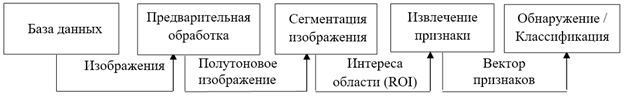
\includegraphics[width=0.8\linewidth]{pic14}
\caption{Основные этапы системы обнаружения и классификация на основе методов компьютерного зрения и машинного обучения.}
	\label{pic14}
	\end{figure}
%%--------2.1-------------%
\section{Предварительная обработка изображения и извлечение признаков в системах ОКДДП и ОКФП}
\subsection{Предварительная обработка изображения в системах ОКДДП и ОКФП}
Процесс обработки изображений считается основой системы. Система должна иметь возможность работать с различным разрешением исходных изображений и работать в режиме времени близкого к реальному. Поэтому процесс обработки изображений должен быть изучен и оптимизирован для того, чтобы система производила качественные результаты, но обеспечивала высокую производительность системы.

Основываясь на выборе методов предварительной обработки, результаты обнаружения и классификации системы значительно улучшены, что увеличивает скорость обработки всей системы. Этот процесс включает в себя фильтрацию шума и получение плавного изображения, выявление признаков объектов на изображении, а затем преобразование изображения в полутоновое изображение (рис. \ref{pic15}). В данной работе использован фильтр Гаусса для удаления шума. Сущность этого преобразования состоит в реализации свертки изображения с ядром симметричной формы в виде 2-D функции Гаусса. Эта непрерывная функция определяется следующим образом:
\begin{equation}\label{eq1}
 f\left(x, y\right) = \frac{1}{2\pi\sigma^2} \exp \left(-\frac{x^2+y^2}{2\sigma^2}\right)
\end{equation}

\begin{figure}[ht!]
\centering
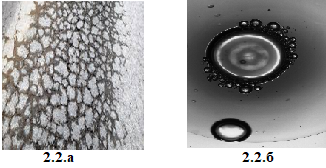
\includegraphics[width=0.5\linewidth]{pic15}
\caption{Результат преобразует изображение в полутоновое изображение (2.2.а - изображение дефектов дорожного покрытия; 2.2.б - изображение пузырьков).}
	\label{pic15}
		\end{figure}

Во время сбора объектов изображения повреждаются шумом, который влияет на обнаружение и извлечение признаков объектов.

Кроме того, условия освещения могут изменять различные области изображения, что приводит к их деградации. Эти проблемы решаются с помощью адаптивной балансировки гистограмм (рис. \ref{pic16}).
\begin{figure}[ht!]
\centering
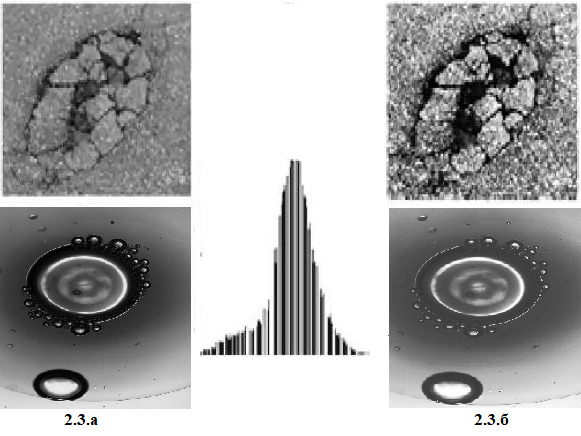
\includegraphics[width=0.5\linewidth]{pic16}
\caption{Результат выравнивания гистограммы.}
	\label{pic16}
		\end{figure}
		
Алгоритм эквализации гистограммы основан на простой идее и часто используется при обработке изображений. Цель эквализации гистограммы, как уже отмечалось выше, заключается в увеличении диапазона яркости изображения.

Эквализация гистограммы изображения g определяется следующим образом:
\begin{equation}\label{eq2}
g_{i,j}=floor \left(\left(L-1\right)\sum^f{i,j}_{n=0} p_n\right)
\end{equation}

\begin{itemize}
	\item $	f$  исходное изображение;
	\item $n=0,1,…,L-1;L [0 ; 255]$;
	\item $p_n$: количество пикселей по интенсивности  n / количество пикселей;
	\item $floor()$ округляется до ближайшего целого числа. Это эквивалентно преобразованию интенсивности пикселей $k \in f$ с помощью функции:
	\begin{equation}\label{eq3}
T\left(K\right)=floor\left(\left(L-1\right)\sum^f{i,j}_{n=0} p_n\right)
\end{equation}
\end{itemize}
Для высокоселективного процесса экстракции в предлагаемой работе используется морфологический метод для выявления дефектов пикселей и удаления небольших участков потенциала шума изображения на изображении (рис. \ref{pic17}). Морфологический метод анализа геометрических структур был разработан для двоичных изображений, а затем расширен до полутоновых изображений. Это один из методов, применяемых на этапе предварительной обработки. Двумя наиболее часто используемыми операциями являются Dilation и Erosion. Из этих двух основных математических операций разрабатывается ряд операций, таких как Close и Open.

\begin{equation}\label{eq4}
I\oplus H = \bigcup_{q \in H} I_q
\end{equation}

\begin{algorithm}[H]
  \KwData{Изображение $I$, структурирующий элемент $H$.}
  \KwResult{Изображение $\acute{I} = I \oplus H$}
 1. Начать с нулевого изображения $\acute{I}$\\
 2. Перебирать все $q \in H$\\
 3. Вычислить сдвинутое изображение $I_q$\\
 4. Обновить $\acute{I} = I \nu I_q $\\
\caption{Алгоритм расширения}\label{alg1}
\end{algorithm}

\begin{algorithm}[H]
  \KwData {Изображение $I$, структурирующий элемент$H$.}
\KwResult: {Изображение $\acute{I} = I \ominus H$}
 1. Начать с инверсии $\acute{I} = \bar{I}$\\
 2. Распространяться $\acute{I}$ with reflected structure element $H^*$\\
 3. Инвертировать $\acute{I}$\\
\caption{Алгоритм эрозии} \label{alg2}
\end{algorithm}

\begin{figure}[ht!]
\centering
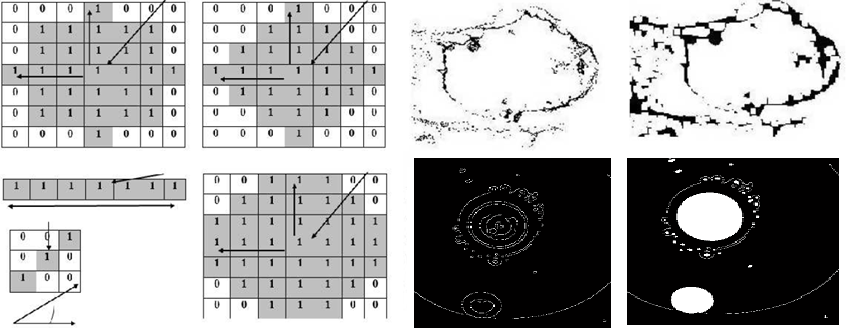
\includegraphics[width=0.7\linewidth]{pic17}
\caption{Результаты морфологических операций.}
	\label{pic17}
		\end{figure}
		
\subsection{Извлечение признаков в системах ОКДДП и ОКФП}

До извлечения признаков предлагется предварительная обработка изображений. Сначала  применяется фильтрация шума с использованием фильтра Гаусса и конвертирование в полутоновые изображения. На следующем шаге выполняется сегментация изображения. Предложено разделение изображения на отдельные области. Затем отделяются пиксели объектов изображения для обнаружения связной области. Используется морфологический метод для обнаружения пикселей соответствующих объектов и для удаления небольших областей, которые определены как шум. 

\textbf{а) Извлечение признаков в системе ОКДДП}.

Рассмотрим следующие дефекты:
 
\textit{Сеть трещин} (рис. \ref{pic18}): Взаимосвязанные трещины, образующие серии блоков приблизительно прямоугольной формы, обычно распределены по всей поверхности дорожного покрытия. Атрибутами блока дефекта трещин  являются: ширина преобладающей трещины $\left(mm\right)$, ширина преобладающей ячейки $\left(mm\right)$, пострадавшая площадь $\left(m^2\right)$.
 
\begin{figure}[ht!]
\centering
\includegraphics[width=0.5\linewidth]{pic18}
\caption{Описание сети трещин.}
	\label{pic18}
		\end{figure}
		
\textit{Глубокие трещины} (рис.\ref{pic19}): Неприсоединенная трещина в продольном направлении вдоль дорожноого покрытия. Атрибуты дефекта продольных трещин : ширина трещин $(mm)$, длина трещин $(m)$, интервал трещин $(mm)$, площадь пострадавших трещин $(m^2)$.

\begin{figure}[ht!]
\centering
\includegraphics[width=0.5\linewidth]{pic19}
\caption{Описание глубоких трещин.}
	\label{pic19}
		\end{figure} 
		
\textit{Выбоины } (рис. \ref{pic20}): углубления некруглой формы различных размеров в дорожном покрытии. Атрибутами дефекта выбоин  являются глубина выбоин $(mm)$ и площадь выбоин $(m^2)$.

\begin{figure}[ht!]
\centering
\includegraphics[width=0.5\linewidth]{pic20}
\caption{Описание выбоины.}
	\label{pic20}
		\end{figure} 

Из анализа атрибутов каждого дефекта, мы выбрали следующие признаки:

\textit{Hu-моменты:} Наиболее заметны Hu-моменты, которые могут быть использованы для описания, характеристики, и определения формы объекта в изображении. Hu-моменты, как правило, извлекаются из формы объекта в изображении \cite{h130}. Описывается форма объекта и извлекается вектор признаков формы (т.е. список чисел) для представления формы объекта. Затем проводится сравниние двух векторов признаков с использованием теории подобия или расстояния функции, чтобы определить, насколько формы анологичны.

\textit{Цепной код гистограммы}: Код цепи гистограммы (CCH-chain code histogram) предназначен для группировки объектов, с исользованием методики, анологичной  наблюдением человека\cite{h131}. Он не предназначен для точного обнаружения и классификации задач. Цепной код гистограммы вычисляется из кодовой цепочки представленного контура.

Код цепи Фримэн \cite{h132} представляет собой компактный способ представления контура объекта. Код цепи представляет собой упорядоченную последовательность $n$ связывает $\left\{c_i, i=1,2,.., n\right\}$, где $c_i$ вектор, соединяющий соседние пиксели контура. Направления $c_i$ кодируются с помощью целых значений $k=0,1,...,K-1$ в направлении против часовой стрелки, начиная от направления положительного $x-axis$. Число направлений $k$ принимает целые значения $2^{M+1}$, где m является положительным целым числом. Цепные коды, где $K>8$, называются обобщенными кодами цепей \cite{h133}.

Расчет кода цепи гистограммы производится быстро и просто. Код цепи гистограммы представляет собой дискретную функцию: $p(k)=n_k/n, k=0,1,...,K-1,$ где $n_k$ является количеством значений кода цепи  $k$ в коде цепи, и $n$ это число звеньев в цепи кода. Кроме этого, рассматривается также размер дефекта области (ширина и длина, площадь) и гистограммы изображения. 

Для автоматического обозначения дефектных областей (или отсутствия дефектных областей), предложена  операционная система распознавания образов  с использованием простого пространства признаков . Пространство признаков многомерно, в этой задаче строятся 4 мерные пространства с использованием областей локальной статистики, вычисленные для нормированных и насыщенных изображений. Первыми признаками является среднее значение всех интенсивностей пикселей в области. Второе пространство признака это цепной код гистограммы, третое - Hu-момент, используемый для описания, характеристики, и определения формы объекта в изображении. В-четвертых, размер дефекта области (ширина, длина, площадь) и гистограмма изображения.
		
\textbf{б) Извлечение признаков в системе ОКФП}

В системе обнаружения и классификации признак формы пузырьков  определяется в сегментации, обнаружении и классификации процессов. Признаки описаны следующим образом:

\textit{Преобразование вейвлет} \cite{15wl}, \cite {16wl} применяется для задачи обнаружения объекта, эффективно работает для полей обнаружения мелких объектов, таких как обнаружение диафрагмы \cite{17wl}, обнаружение газового пузыря \cite{18wl} и т.д. Алгоритм вейвлет-преобразования является хорошим вариантом для оценки пузырьков воздуха в сложных полевых условиях сигналов с большим шумом. Общий подход заключается в следующем:
\begin{itemize}
	\item Исходное изображение разлагается и реконструируется в вейвлет. Оно включает в себя низкочастотное изображение и высокочастотные изображения - оно может быть объектом, которое необходимо обнаружить на изображении.
	\item Затем снижается низкочастотное изображение, а высокочастотные изображения группируются в новое изображение.
	\item Новое изображение сегментируется порогом, затем объект распознается и помечается.
\end{itemize}

Хаара-Вейвлет является одним из типов вейвлет-преобразования, который был выбран в качестве признака для извлечения. Он обладает свойствами пространственно-частотной локализации и настраиваемых деталей. 
Для вейвлета Хаара функция масштабирования$\phi\left(x\right)$ определяется как:

\begin{equation} \label{eq5}
\phi\left(x\right)= \left\{\begin{array}{l} 1, if x \in \left[0,1\right],\\
0, if x \notin \left[0,1\right],
\end{array}\right.
\end{equation}

Вейвлет-функция $\varphi\left(x\right)$ поскольку эта функция масштабирования определяется как:

\begin{equation} \label{eq6}
\varphi\left(x\right)= \left\{\begin{array}{l} 1, if x \in \left[0,0.5\right],\\
-1, if x \in \left[0.5,1\right],\\
0, if x \notin \left[0,1\right]
\end{array}\right.
\end{equation}

\textit{Признаки формы, геометрия, текстура}, такие как: яркость, обнуление значения пикселя, среднее различие между соседними пикселями, площадь, периметр, радиус, длина, ширина, длина / ширина.

%-----------------------------------------------
\section{Математическое моделирование и численные методы для сегментации изображений в системах ОКДДП и ОКФП} \label{part2}
\textbf{Математическое моделирование и численные методы для сегментации изображений}

Рассмотрим изображение $Y$ размера $M \times N$. $S = \left\{s\right\}$ - это множество всех расположений пикселя, $s \left(i, j\right)$ - позиция пикселя. Для каждого расположения $s$ существует значение $x_s=\left\{0;1\right\}$, которое определяет состояние пикселя в позиции $s$ какой-то области. Результатом сегментации являются наборы ROI (\ref{pic21}): $\bigcup\ s_{i,j} | x_{s_{i,j}}=1$.

\begin{figure}[ht!]
\centering
\includegraphics[width=0.7\linewidth]{pic21}
\caption{Описание дефектов дорожного покрытия.}
	\label{pic21}
		\end{figure} 
		
\textbf{Численный метод для сегментация изображения на основе разреза на графах и MRF}
\subsection{Численный метод для построения карты дефектов дорожного покрытия}
Обнаружение дефектов дорожного покрытия, где области изображения помечены как содержащие дефектные пиксели или не содержащие и  выявление типа классификации дефектов дорожного покрытия, где каждому выявленному дефекту дорожного покрытия присваиваются метки «блок трещины», «продольные трещины», «выбоины». Для обнаружения дефектов дорожного покрытия,необходима начальная настройка , когда оператор выбирает изображения, используемые для определения оптимального набора параметров обнаружения, приходящихся на пиксель, следующий за пикселем серой шкалы вариации, связанные с контрастом, яркостью и состоянием поверхности дефекта дорожного покрытия. На этом этапе установки, программа обеспечивает визуальную обратную связь с результатами обнаружения в виде дефектных карт основных изображений, прошедших контроль дорожных покрытий.		
	
В настоящем исследовании метод разрезов на графах применен для решения задач сегментации изображений которые имеют сложную структуру на основе анализа соотношения компонентной связности между пикселами для построения карты дефектов \cite{h144,h145}. Построение карты дефектов дорожного покрытия -- суть маркировка пикселей на изображении значением (0 - не дефектом; 1-пиксельный дефект) и выполняется в 3 шага:

\begin{itemize}
	\item \textit{Шаг 1}. Используя метод разреза на графах изображение сегментируется и извлекается область интереса (region of interest -- ROI).
\item \textit{Шаг 2}. Результат сегментации дефектов в ROI улучшается с использованием модели марковских случайных полей.
\item \textit{Шаг 3}. Построение полной карты дефектов путем сравнения и замены пиксельных меток, которые получены из шагов 1 и 2.
\end{itemize}

\textbf{Сегментация изображения алгоритмом минимального разреза -- максимального потока.} Применили метод на основе эффективного графика, чтобы найти оптимальное $D$ (дефект) - $N$ (не дефект). На рис.\ref{pic25} представлен обмен между областями $N$ и $D$ - расширение данной маркировки $f$. Предложено использование алгоритма разреза на графах, чтобы эффективно найти $f$ \cite{h13}. Использовали краткий подход. Пусть $G=\left(V,E\right)$ как взвешенный граф с двумя отмеченными вертикалями называются терминалами. Разрез $C \in E$ является множеством ребер, таких, что терминалы разделены в наведенном графе $G\left(C\right)=\left\langle V,E-C\right\rangle$. Кроме того, ни одно подмножество $С$ не разделяет терминалы в $G\left(C\right)$. Стоимость разреза $C$, обозначается $|C|$, и равна сумме его весовых значимостей.

\begin{figure}[ht!]
\centering
\includegraphics[width=0.5\linewidth]{pic25}
\caption{Использование разреза графа для улучшения сегментации изображения}
	\label{pic25}
		\end{figure} 

\begin{algorithm}[ht!]
  \KwData{ Граф $G\left(V,E\right)$ с емкостью $c$, исток $s$, сток $t$.}
  \KwResult{Максимальный поток от источника $\left(s\right)$ до стока $\left(t\right)$}
		1. \For{\texttt{$i := 1$ для всех ребер $\left(u,v\right)$ }}
     {
		$f\left(u,v\right) \leftarrow 0$
		}
	
		2. \eIf{$c_f\left(u,v\right) > 0$ для всех ребер $\left(u,v\right) \in p$}{
      $c_f\left(p\right) = min \left\{c_f\left(u,v\right)| \left(u,v\right) \in p\right\}$;
    }{
       todo 1;
    }
		3. \For{\texttt{$i := 1$ для всех ребер $\left(u,v\right)$ }}
     {
		$f\left(u,v\right) \leftarrow f\left(u,v\right) +c_f\left(p\right) $;
		}		
  \caption{Описание алгоритма разрезов на графах} \label{alg3}
\end{algorithm}

Подход на основе граф дает возможность использования эффективных решений задачи минимального разреза -- максимального потока между источником и приемником узлов ориентированных граф. Проблема минимального разреза в том, чтобы найти самый оптимальный срез среди всех разрезов, разделяющих сегменты. Минимальные разрезы могут быть эффективно найдены с помощью стандартных комбинаторных алгоритмов с различными полиномиальными сложностями низкого порядка \cite{h137}. Экспериментальные результаты были получены с помощью использования нового алгоритма минимального разреза -- максимального потока, имеющего лучшую скорость на графах для решения многих современных алгоритмов \cite{h138}. Цель заключается в сегментации изображений путем построения графа таким образом, что минимальный разрез этого графа мог вырезать все ребра, соединяющие пиксели различных объектов друг с другом (рис.\ref{pic22}).
\begin{figure}[ht!]
\centering
\includegraphics[width=0.5\linewidth]{pic22}
\caption{Сегментация изображения дефектов дорожного покрытия.}
	\label{pic22}
		\end{figure} 
		
\textbf{Оптимизация сегментации изображений на основе алгоритма Марковских случайных полей}. Для повышения качества сегментации изображений используется алгоритм Марковского случайного поля \cite{h134}. Использование SA \cite{h139, h140} для создания Марковского процесса для модели MRF, которая применяется к изображению.


\begin{itemize}
	\item \textit{Шаг 1}. Выполнить случайно M-решения для сегментов из исходного изображения.
	\item \textit{Шаг 2}. Выбрать начальное решение, называемое $X_0$. Вычислить стоимость $U \left(X_0\right)$.
	\item \textit{Шаг 3}. Повторить с оставшимся раствором $M-1$. С решением $X_i$:
	
	\begin{itemize}
		\item Вычислить стоимость $U\left(X_0\right)$.
		\item Сравнить $U\left(X_i\right)$ и $U\left(X_0\right)$. Увеличить $m_1$ если $U\left(X_i\right) < U\left(X_0\right)$, иначе увеличить $m_2$.
	\end{itemize}
Где  $m_1$: количество рекомендуемых переходов $x \rightarrow y$ так что $U\left(y\right) \leq U\left(x\right)$ (принять); 
	   $m_2$: количество рекомендуемых переходов $x \rightarrow y$ так что $U\left(y\right) \leq U\left(x\right)$ (понесено случайно) 
	\item Вычислить $^{\Delta_U}$ на $U\left(X_i\right) > U\left(X_0\right) $. 
	Где $^{\Delta_U}$ средняя стоимость минус $m_2$
	\item Вычислить $\chi \left(T\right) = \frac{m_1}{m_1+m_2}$
\end{itemize}

После выполнения алгоритма SA, полученного в модели MRF, эта модель представляется как взаимодействие между соседними пикселями. Этот сегмент изображения демонстрирует различие между большими дефектными областями и дефектами мелкой области на основе взаимодействия пикселей для группировки пикселей вместе (рис.\ref{pic23}). Преимущество использования этой модели заключается в том, что она удаляет мелкие детали или объединяет меньшие части в большую часть в процессе сегментации, чтобы идентифицировать наиболее дефектные области.

\begin{figure}[ht!]
\centering
\includegraphics[width=0.7\linewidth]{pic23}
\caption{Сегментация изображения дефектов дорожного покрытия на основе взаимодействия пикселей.}
	\label{pic23}
		\end{figure} 
		
\textbf{Алгоритм изменения перемещения и расширения для получения полной карты дефектов дорожного покрытия}. Эти сегменты называются «участками» и имеют предварительно определенную ориентацию 0, 45, 90 или 135 градусов. Разделение между обоими случаями осуществляется с помощью параметра $k \in \left(0,1\right)$. 

Эти дефектные карты обеспечивают мгновенную обратную связь с эффективностью параметров. Посредством итеративного процесса, оптимальные параметры обнаружения выбираются для каждого управления дорожного покрытия. После  выбора настройки, программа будет автоматически обрабатывать изображение дорожного покрытия для обнаружения дефектов. Для каждого дефекта, длина, ширина и ориентация вычисляются и сохраняются. Примером является цифровая карта дефектов, которая демонстрирует карту дефектов, соответствующую изображению.

\begin{algorithm}[H]
 1.Начать с произвольной маркировки. $f$\\
 2.Установить переменную success:= 0\;
 3.\For{\texttt{каждая пара метки ${D, N} \subset L$}}
     {
		Найти $\hat{f} = argminE(\acute{f})$ среди $\acute{f}$ в течение одного $D-N$ перекачка $f$\;
		\If{$E( \hat{f}) < E(f)$}{
   задавать $f := \hat{f}$\;
	 success := 1\;
   }
		}
4.\If{success = 1}{
   идти к 2\;
   }
5.Вернуть $f$
\caption{Шаги изменения алгоритма  перемещения и расширения.} \label{alg4}
\end{algorithm}

Время работы близко к линейному на практике. Некоторые результаты сегментации классов дефектов дорожного покрытия показаны на рис.\ref{pic24}.

\begin{figure}[ht!]
\centering
\includegraphics[width=0.7\linewidth]{pic24}
\caption{Результаты сегментации классов дефектов дорожного покрытия.}
	\label{pic24}
		\end{figure}
%--------------------------------------------------------
\subsection{Численный метод для обнаружения пузырьков}
Пусть графа $ G = \left\{V, E \right\} $ строится узлами $ V $ и ребрами $ E $. Рассмотрены пиксели изображения как узлы, два дополнительных узла $ S $ (источник) для объектов-пучков и $ T $ (терминал) для фона. Для построения взвешенного графа из изображения (рассматривается система $ d = \left(4,8 \right) $ - окрестности). Для каждой пары узлов t-link - это ребра. Функция веса присваивается каждой t-ссылке $ \left (B_ {p, q} \right) $  и приведится ниже.

\begin{equation} \label{eq9}
B_{p,q}= \exp - \frac{\left(I_p - I_q\right)}{2\sigma^2} \frac{1}{dist\left(p,q\right)}
\end{equation}

Где $ B_ {p, q} $ - измерение сходства интенсивностей изображения в пикселях $ p $ и $ q $. Для параметров инициализации алгоритма разреза на графах выбирается набор пикселей на переднем плане (объекты-пузырьки) и фон. Интерактивная сегментация учитывает мягкие ограничения (граничные и региональные свойства сегментов). Вес определяется отрицанием сходства. Область сегментации определяет инициализированные регионы на основе выбранных гистограмм.


\begin{equation} \label{eq10}
\left\{\begin{array}{l} W_p\left('FG'\right)=-\ln His\left(I_p|O\right),\\
W_p\left('BG'\right)=-\ln His\left(I_p|B\right),
\end{array}\right.
\end{equation}

Где $ His \ left (I_p | O \ right) $, $ His \ left (I_p | B \ right) $ - гистограммы интенсивности объекта и фона соответственно. Весы по краям графа назначаются в соответствии с алгоритмом разреза на графах (Алгоритм \ref{alg3}). Графический подход использует эффективные решения проблемы минимального разреза -- максимального потока между узлами источника и приемника в ориентированных графах.

В работе используется алгоритм минимального разреза -- максимального потока для реализации сегментации изображения пузырьков. В данном исследовании реализован этот алгоритм, который получен из реализации алгоритм минимального разреза -- максимального потока. На рис.\ref{pic30} показан результат построения карты с помощью признаков текстуры.

\begin{figure}[ht!]
\centering
\includegraphics[width=0.8\linewidth]{pic30.png}
\caption{Признаки текстуры, используемые при сегментации изображения.}
	\label{pic30}
	\end{figure}
	
	Результат сегментации изображения пузырьков с использованием базы данных текстуры на основе алгоритма разреза на графах (рис.\ref{pic31}). Изображение сегментируется в область для извлечения признаков пузырьков.
\begin{figure}[ht!]
\centering
\includegraphics[width=0.8\linewidth]{pic31.png}
\caption{Результат сегментации изображений пузырьков алгоритмом разреза на графах.}
	\label{pic31}
	\end{figure}

В предлагаемом методе используется алгоритм обнаружения пузырьков, основанный на вейвлет-преобразовании Хаара. Этот метод применяется к каждой области интереса - ROI, полученной из сегментации изображения с помощью разрезов на графах. Характерный признак вейвлет-преобразования Хаара является разделимым и легко вычисляется. В этом случае пузырьки воздуха в процессе являются ключевым изменением параметра. Следовательно, вейвлет-коэффициенты могут быть лучшим представлением сигнала, чем выборки во временной области.

Процесс извлечения объектов в изображениях на основе преобразований Хаара-Вавелета (рис.\ref{pic32}) выполняется алгоритмом \ref{alg5}.

\begin{algorithm}[ht!]
  \KwData{N изображений.}
  \KwResult{Значения вейвлет-преобразования Хаара (коэффициенты)}
		1. Преобразование изображения RGB в полутоновое изображение;
		
		2. Изменить размер изображения на $128 \times 128$;
		
		3. Предварительная обработка (фильтрация шума, морфологическая обработка)
		
		4. Вейвлет-преобразование для создания вектора $\vec{I_i}, i=1..N$;
		
		5. Среднее значение: $I_N=\frac{1}{N}\sum_{i=1}^N I_i$
		
		6. Расчет для каждого объекта: $\vec{u_i}=\sum_{k=1}^N V_{ik} \phi_k, i=1..N$\\
		$\phi_k=\vec{I_i}-\vec{I_N}$: вычитание среднего изображения из каждого изображения.
			$V_{ik}$: вектор каждой матрицы $W^tW, W=\left\{\vec{\phi_1},...,\vec{\phi_N}\right\} $
  \caption{Извлечение признаков пузырей вейвлет-преобразованием Хаара}\label{alg5}
\end{algorithm}

Для сравнения полученных значений вейвлет-преобразования Хаара используется универсальный порог $ T = \sigma \sqrt {2 \ln n} $, где $ \sigma $ - среднее абсолютное отклонение, а $ n $ - количество выборок конкретных коэффициентов вейвлет-преобразования. Частота дискретизации и масштаб вейвлет-разложения фиксированы $ T = k \sigma $, где $ k = \sqrt {2 \ln n} $ является параметром.
\begin{figure}[ht!]
\centering
\includegraphics[width=0.7\linewidth]{pic32}
\caption{Анализ с использованием вейвлет-преобразования Хаара для потока сигнала с пузырьками}
	\label{pic32}
	\end{figure}

Вейвлет-преобразование Хаара извлекается и создается вектор из подробного коэффициента, который вычисляется путем адаптивного порога. Порог проверяется на подробные коэффициенты. Если подробные коэффициенты превышают порог в конкретном случае, можно сделать вывод, что обнаружены пузырьки воздуха (рис.\ref{pic33}).
\begin{figure}[ht!]
\centering
\includegraphics[width=0.8\linewidth]{pic33}
\caption{Результат обнаружения пузырьков с использованием вейвлет-преобразований Хаара с измерением радиуса объекта.}
	\label{pic33}
	\end{figure}

\textbf{Классификация формы пузырьков на основе радиуса признак}

Пузырьки всегда существуют во множестве (fig.\ref{fig11})  разновидностей:одиночные, перекрывающиеся, погруженные в жидкость или растворенные в окружающей среде.
\begin{figure}[ht!]
\centering
\includegraphics[width=1\linewidth]{p11.png}
\caption{Типы существующих пузырьков.}
	\label{fig11}
	\end{figure}
	
Классификацию пузырей проводим на основе особенностей радиуса. Проводим сравнение расстояния между центром и радиусом пузырей, рассматривая окружающие пузыри. Если центр тяжести больше или равен радиусу, то пузыри существуют в единственной форме, иначе перекрываются.

%---------------------------------------------------------
\section{Математическое моделирование и численные методы для классификации объектов}
\subsection{Проблема несбалансированности данных в классификации объектов}

Данные несбалансированности исходят из идеи чувствительной стоимости изучения, в таком случае случайный лес больше подходит для изучения. Класс весового значения является важным параметром настройки для достижения желаемой производительности. В процедуре построенния дерева индукции, критерий Джини используется при  определении весового значения, чтобы находить расколы. В концевых узлах каждого дерева, вновь принимается во внимание весовой класс . Введем понятие \cite{h143}: Правильный позитив (True Positive - TP) - правильно классифицирован как положительный, правильный негатив (True Negative - TN) - правильно классифицирован как негативный, неправильный позитив (False Positive – FP) - классифицирован неправильно как положительный, неправильный негатив (False Negative - FN) - ошибочно классифицируется как негативный. Для алгоритма случайного леса, всегда существует компромисс между правильным позитивом  и правильным негативом и то же самое применяется для отзыва и точности.

Правильный негатив ставки $=\frac{TN}{TN+FP}$, Правильный позитив ставки $=\frac{TP}{TP+FN}$, Точность $=\frac{TP}{TP+FP}$

\textbf{Несбалансированность данных в классификации дефектов дорожного покрытия}. Обучающий набор состоит из 500 изображений (200 классов «дефектов» и 300 классов «без дефектов» (таб. \ref{tab3}). В 200 изображений классов дефекта включены 150 изображений (50 сеть трещин, 50 глубокие трещины, 50 выбоины изображений) для тренировочного процесса и 50 изображений для процесса тестирования. В 300 изображениях класса без дефектов включены 200 для процесса обучения и 100 изображений для процесса тестирования. Данные изображения были построены с помощью «центра телекоммуникаций и мультимедиа», INESC TEC, Португалия и наш собственный набор данных, который собирается с помощью камеры (Canon D100 16 Мп). Изображения захватываются в обычном состоянии дневного света, расстояние от камеры до поверхности дороги 1м-1.2м. Затем изображения обрабатываются с разрешением (256 * 256) пикселей и (500 * 500) пикселей.

	 \begin{table}[h!]%
\centering
\caption{Лучшая модель для классификации зависит от точности, истинной положительной ставки, ложной положительной ставки в системе ОКДДП.}
\label{tab3}
  \begin{tabular}{|c|c|c|c|}
    \hline														
     \multirow {2}{*}    {Класс}      & {Истинно}            & {Ложно}          & {Точность}\\
		                                  & {положительный}      & {положительный}  &{}\\
    \hline
Выбоины                   &0.903 	&0.556 	&0.843\\
\hline 
Сеть трещин 	&0.80 	&0.726 	&0.880\\
\hline 
Глубокие трещины	&0.947 	&0.230 	&0.926\\
\hline 
  \end{tabular}
\end{table}%\vspace{10mm}

%\textbf{Несбалансированность данных в классификации формы пузырьков}. Данные включают в себя 2 изображений База данных <<ShellScratch>> и <<TrueTear>> (таб. \ref{tab31}) , которые полностью описывают информацию в формате * .png и разрешение 1300 * 1030 пикселей, предоставленное лабораторией в Сингапуре. Данные разделены на две части: 2/3 данных для обучения и 1/3 данных для тестировани данных. Затем изображения будут уменьшены в размере до того же разрешения (128 * 128) или (256 * 256). Диапазон размеров для пузырьков составляет $>$ 1 пиксель, а форма пузырька $>$ 10 пикселей.
%
	 %\begin{table}[h!]%
%\centering
%\caption{Лучшая модель для классификации зависит от точности, истинной положительной ставки, ложной положительной ставки в системе ОКФП.}
%\label{tab31}
  %\begin{tabular}{|c|c|c|c|}
    %\hline														
     %\multirow {2}{*}    {База данных}      & {Истинно}            & {Ложно}          & {Точность}\\
		                                  %& {положительный}      & {положительный}  &{}\\
    %\hline
%ShellScratch                &0.910 	&0.603 	&0.925\\
%\hline 
%TrueTear	&0.928 	&0.176 	&0.944\\
%\hline 
%
  %\end{tabular}
%\end{table}%\vspace{10mm}
%------------------------------------------------------------
\subsection{Математическое моделирование и численные методы для классификации объектов в системе ОКДДП}
\textbf{Математическое моделирование для классификации объектов в системе ОКДДП}

Пусть $S=\left\{X, Y\right\}$ - множество N обучающих выборок, набор дефектов дорожного покрытия признаков $X=\left\{x_i | i = 1, ..., 5\right\}$ и набор меток классов $Y = \left\{y_i |i = 1, ..., 3\right\}$. Классификатор - это функция $H: X \rightarrow Y$, которая отображает $x$ в элемент $y$ из $Y$. Это значит, построение модели обучения и тестирования для классификации объектов по меткам $Y$.

Используется алгоритм случайного леса для классификации дефектов: сети трещин, глубоких трещин и выбоин. Таким образом, каждое дерево строится на множестве $N_t$, это множество случайным образом выводится из $N$. Данные обучения $N_p$ узла $p$ делятся на два набора: $N_l$ - слева и $N_r$ – справа должны следовать пороговое значение $c$ характеристического вектора $v$ в функции $f$:
\begin{equation}\label{eq11}
N_l = \left\{n \in N_p | f\left(v_n\right) > c\right\};  \\
N_r=N_p / N_l.
\end{equation}
На каждом узле создается группа $ m $ -функции, которая случайным образом предлагается для функции $ f $ и находит все возможные значения $ c $ и выбирает из них значение. Чтобы получить самый высокий индекс Джини \cite{19wl}:
\begin{equation}\label{eq12}
\Delta I_G\left(N_p\right)=I_G\left(N_p\right) - \frac{|N_l|}{|N_p|}I_G\left(N_l\right) - \frac{|N_r|}{|N_p|}I_G\left(N_r\right), 
\end{equation} где $I_G\left(N\right)$ - индекс Джини для данных изучения $N$.

\textbf{Численный метод для классификации на основе алгоритма случайного леса}.

Случайный лес - это метод машинного обучения, основанный на комбинированном обучении, который является методом создания множественных классификаторов и синтезирует их результаты для получения конечного результата.

Случайный лес генерирует множество деревьев решений, а именно алгоритм классификации и регрессии (CART) и использует метод Bagging. Каждое дерево обучается с помощью бутстрапа, который получен из исходного набора данных. Для создания методов обучения и тестирования в случайном лесу использовалась техника «Out-Of-Bag».

Численный метод основан на алгоритме случайного леса (алг.\ref{alg4}) для решения проблемы классификации дефектов дорожных покрытий в системе ОКДДП.
\begin{algorithm}[ht!]
  \KwData{$T$ - количество деревьев; $N$ - количество выборок из набора данных.}
  \KwResult{$y\left(x_i\right)$ - метка для объекта}
   1. \For{\texttt{$t := 1$ to $T$ }}
     {
		1.1 Создавать $M$ - новый шаблон данных с $n$ - размер $M$ из исходного набора данных $N$;
		
		1.2 Создавать дерево классификаторов для каждого$M$;
		
		1.3 \For{\texttt{$i := 1$ ко всем узлам}}
     {
		  1.3.1 Получить случайные  $mtry$ признаки из оригинальной функции;
			
			1.3.2. Выбор лучшего раскола в $mtry$ признаке;
		}
		1.4 $y\left(x_t\right)$ = метка $t$ дерева; 
		}
		
		2. Вернуть $y\left(x_i\right)$ = $\left\{y\left(x_t\right)\right\}^T$ - большинство голосов;
		
  \caption{Классификация объектов на основе алгоритма случайного леса.}\label{alg4}
	
\end{algorithm}

В данном разделе описывается классификация, основанная на методе обучения с учителем (рис. \ref{pic26}) -- алгоритм случайного леса в дальнейшем принимает концепцию дерева решений, производя большое количество деревьев решений. Сначала извлекается случайная выборка данных и определяется ключевой набор признаков, чтобы вырастить каждое дерево решений. Эти деревья решений, то есть их «Out-Of-Bag» определяют ошибку (частота ошибок модели), а затем ряд деревьев решений сравнивается, чтобы найти совместный набор переменных, которые производят самую точную модель классификации.

\begin{figure}[ht!]
\centering
\includegraphics[width=0.9\linewidth]{pic26}
\caption{Блок схема классификации объектов в системе ОКДДП.}
	\label{pic26}
		\end{figure}	
		
%Классификатор Random Forest был построен с использованием пакета Random Forest 4.5-16 для статистической среды \cite{h142}, чтобы классифицировать векторы признаков по наличию дефекта. Классификатор прошел обучение по набору данных для дорожного покрытия  с помощью цепного кода гистограммы - CCH, Hu-момент, размер дефекта для каждого случая в системе ОКДДП.
%
%В системе ОКФП использовался алгоритм случайного леса (алг.\ref{alg4}), чтобы классифицировать форму пузырьков с целью обнаружения метки между двумя пересекающимися пузырьками. Вектор признаков создается извлеченными значениями  признаков, которые являются: признаками текстуры, признаками геометрии, спектральными признаками. Объект на изображении будет помечен двумя метками $ \left\{- 1; +1\right\}$.
%------------------------------------------------
\section{Применение методов и алгоритмов компьютерного зрения и машинного обучения для обнаружения и классификации объектов на изображениях}
В этом разделе описывается процесс применения алгоритмов и методов машинного обучения \ref{pic27} для извлечения дефектов дорожного покрытия (гистограмма цепного кода, локальные шаблоны, размер дефекта области – ширина, длина, площадь), построение карты дефектов дорожного покрытия и классификация данных представлена в разделе \ref{partc} ; обнаруживается радиус пузырька, классифицируется форма пузырька в системе, как показано в разделе \ref{partd}.
\begin{figure}[ht!]
\centering
\includegraphics[width=0.8\linewidth]{pic27}
\caption{Блок-схема обнаружения и классификации объектов в системе ОКДДП и ОКФП.}
	\label{pic27}
		\end{figure}
%----------------------------------
\subsection{Применение методов и алгоритмов компьютерного зрения и машинного обучения для обнаружения и классификации дефектов дорожного покрытия  на изображениях в системе ОКДДП} \label{partc}
В результате проведенного анализа в разделе \ref{part2} установлено, что основы метода машинного обучения включают в себя следующие этапы (рис \ref{pic28}) для обнаружения и классификации дефектов дорожного покрытия:

\begin{itemize}
	\item \textbf{Шаг 1 предварительная обработка изображения}
	
	\begin{itemize}
	\item преобразование в полутоновое изображение;
	\item изменение размера изображение до $512*512$ пкс;
	\item Подавление шума линейным фильтром Гаусса; 
	\item баланс гистограммы;
	\item использование морфологических операторов -- дилатаций, чтобы улучшить качество точек изображения со структурами элементов.
	\end{itemize}

\item \textbf{Шаг 2 сегментация изображения и постройние карты дефектов дорожного покрытия}

\begin{itemize}
	\item сегментация изображения алгоритмом минимального разреза -- максимального потока;
	\item оптимизация сегментированного изображения на основе алгоритма случайных полей Маркова;
	\item алгоритмы изменения перемещения и расширения для получения полной карты дефектов дорожного покрытия.
\end{itemize}

\item \textbf{Шаг 3 извлечение признаков}

\begin{itemize}
	\item гистограмма ценпного кода;
	\item ланкальные бинарные шаблоны;
	\item размер дефекта области (ширина, длина, площадь);
	\item создание антропометрического вектора признаков.
\end{itemize}
\item \textbf{Шаг 4 классификация типов дефектов дорожного покрытия по новым данным}
 
 \begin{itemize}
	 \item процесса обучения;
	 \item процесса тестирования;
 \end{itemize}

\end{itemize}
\begin{figure}[ht!]
\centering
\includegraphics[width=0.8\linewidth]{pic28}
\caption{Блок-схема обнаружения и классификация дефектов дорожного покрытия в системе ОКДДП.}
	\label{pic28}
		\end{figure}

%------------------------------------
\subsection{Применение методов и алгоритмов компьютерного зрения для обнаружения и классификации формы пузырьков на изображении в системе ОКФП} \label{partd}
В данной работе рассматривается задача извлечения  признаков пузырьков на изображениях. Для решения этой задачи предложен алгоритм, основанный на совместном применении предложенного алгоритма машинного обучения компьютерного зрения и техника анализа изображения (рис. \ref{pic29} описывает основные этапы этого процесса. 

\begin{itemize}
	\item \textbf{Шаг 1 предварительная обработка изображения}
	
	\begin{itemize}
	\item преобразование в полутоновое изображение;
	\item изменение размера изображения на $128 \times 128$;
	\item подавление шума линейным фильтром Гаусса; 
	\item баланс гистограммы;
	\item обнаружение кромок - алгоритм Canny;
	\item использование морфологических операторов.

	\end{itemize}

\item \textbf{Шаг 2 сегментация изображения и обнаружение пузырьков}

\begin{itemize}
	\item сегментация изображения алгоритмом минимального разреза -- максимального потока;
	\item извлечение признаков пузырей вейвлет-преобразованием Хаара;
	\item сравнение со значением адаптивного порога.

\end{itemize}

\item \textbf{Шаг 3 извлечение признаков}

\begin{itemize}
	\item спектральный признак;
	\item геометрический признак;
	\item структурный признак;
	\item создание антропометрического вектора признаков.
\end{itemize}
\item \textbf{Шаг 4 классификация формы пузырьков с новыми данными}

\end{itemize}
\begin{figure}[ht!]
\centering
\includegraphics[width=0.8\linewidth]{pic29}
\caption{Блок-схема обнаружения и классификация формы пузырьков в системе ОКФП.}
	\label{pic29}
		\end{figure}
%%---------2.5------------------%
\section{Основные результаты и выводы по главе 2}

\begin{enumerate}
	\item В главе 2 представлено математическое моделирование, численные методы, основанные на методах компьютерного зрения и машинного обучения, комбинированные методы обработки изображений для решения проблемы обнаружения и классификации объектов в системах ОКДДП и ОКФП.
\item  В главе 2 основное внимание уделялось задачам обработки данных, предварительной обработки изображений, улучшению качества входных данных с помощью алгоритмов обработки изображений. Оценивалась база данных, собранную для системы обработки.
\item В этой главе были представлены математические модели и численные методы, основанные на алгоритме разреза на графах и алгоритме случайного Марковского поля для сегментирования изображений и получения интересующих областей - областей изображения, которые могут содержать объекты, подлежащие рассмотрению: дефекты дорожного покрытия, пузырьки воздуха.
\item В исследовании представлены признаки объектов двух систем (дефекты дорожного покрытия, пузырьки воздуха) и метод извлечения признаков.
\item В этой главе построена математическая модель и используется численный метод, основанный на алгоритме случайного леса, для классификации объектов.
\item Подробное описание шагов процесса обнаружения и классификации объектов в ОКДДП и ОКФП представлено на изображении.
На основе результатов сбора и предварительной обработки изображений, улучшения изображения, извлечения признаков, математического моделирования и численных методов подробно описаны реальные этапы работы. Целью исследования является обнаружение и классификация объектов на изображении в главе \ref{chapt2}. Исследовательская работа по созданию программы, объединяющей автоматическое обнаружение и классификацию объектов на изображении, представлена в главе \ref{chapt3}.

\end{enumerate}


%%%%%%%%%%%%%%%%%%%%%%%  ГЛАВА 3 %%%%%%%%%%%%%%%%%%%%%%%%%%%%%%%%%%%%%%%%%
\chapter{Реализация методов компьютерного зрения и машинного обучения для классификации объектов в системах ОКДДП и ОКФП} \label{chapt3}
В этой главе дается описание реализации алгоритмов и методов машинного обучения для построения систем ОКДДП и ОКФП для которых в главе 2 были разработаны соответствующие математические модели. Описана структура программ ОКДДП и ОКФП и приведены результаты экспериментов для оценки разработанного метода обнаружения и классификации данных на изображении. Проанализирована эффективность предлагаемого метода в сравнении с другими передовыми методами. 
%%---------3.1-----------------%
\section{Структура программы обнаружения и классификация объектов в системах ОКДДП и ОКФП}
Программная система состоит из 5 модульных структур, которые предствляются структура программ ОКДДП (рис. \ref{pic47}) и ОКФП (рис. \ref{pic59}). Структура системы предназначена для обеспечения того, чтобы каждый модуль имел работающие функции для выполнения одной и той же задачи и мог расширять сферу разработки системы научно обоснованным образом.

\begin{figure}[ht!]
\centering
\includegraphics[width=1\linewidth]{pic47}
\caption{Структура ПО системы ОКДДП}
	\label{pic47}
		\end{figure} 
		
\begin{figure}[ht!]
\centering
\vspace{-0.8em}
\includegraphics [width=0.8\linewidth]{images/pic59.png}
%\captionsetup{justification=justified, labelsep=period}
\caption{Структура ПО системы ОКФП} \label{pic59}
\end{figure}
В качестве входных данных для обнаружения и классификации объектов используются изображение. Процесс улучшения качества изображения и повышения эффективности последующих процессов. Сегментация изображений определяет области изображения, называемые областями интереса (ROI) - местами с высокой вероятностью содержащихся объектов. Эти регионы будут обрабатываться на этапе извлечения признаков, чтобы создать вектор признаков, который содержит описательные значения для каждого типа объектов. Наконец,  признаки были извлечены из объектов, эти объекты проходили процесс классификации, чтобы увидеть, какому классу принадлежит объект, какой тип дефекта, какая форма пузыря.
%-------------3.1.1
\subsection{Модуль ввода/вывода данных}
Блок ввода данных в системе выполняет задачи: хранения изображений, корректировки формата и размера базы данных в стандарте, ввода параметров для алгоритма, отображения результатов системы.

Класс «InOutData» используется для хранения изображений и результатов системы. Структура класса приводится «InOutData» на рис.\ref{pic34}. Класс «InOutData» приведен в таб.\ref{tab5}.

\begin{figure}[ht!]
\centering
\includegraphics[width=0.5\linewidth]{pic34}
\caption{Структура класса InOutData.}
	\label{pic34}
		\end{figure}
		
\begin{table}[h!]%
\centering
\caption{Основные переменные и функции класса InOutData.}
\label{tab5}
  \begin{tabular}{|c|c|}
    \hline
           Название переменной и функции  & Описание \\
\hline 
 \multirow {2}{*}    {inImg: Image  }      & {Переменное хранение}\\
		                                       & {входных изображений.}\\

\hline 
\multirow{2}{*} {outImg: Image} 	         &{Переменное хранение}\\
																					&{выходных изображений.}\\
\hline 
\multirow{2}{*} {label}	                  &{Метка обрабатываемого}\\ 
																					&{объекта.}\\
\hline 
\multirow{2}{*} {LoadData()}	             &{Функция ввода данных}\\
																					&{в систему.}\\
\hline 
\multirow{2}{*} {ReturnData()}	           &{Функция вывода данных}\\
																						&{в систему.}\\
\hline 
  \end{tabular}
\end{table}%\vspace{10mm}
%-------------3.1.2
\subsection{Модуль предварительной обработки изображения}
Блок предварительной обработки изображения можно рассматривать как первый блок в системе для обнаружения и классификации объектов на изображении. Из-за этого точность данного блока будет предоставлять данные для сегментации изображения и обнаружения объектов, извлеченных признаков блоков. Это существенно влияет на эффективность и надежность всей системы обработки.

Технология обработки изображений включает в себя: фильтрацию шума, балансировку гистограмм, обнаружение границ и морфологические операции  для получения изображений хорошего качества, совершенного периметра и полного формата.

Класс «PreProcessImg» предназначен для обработки изображений. Этот класс включает такие процессы, как коррекцуию размера изображения, фильтрацию шума, морфологию, балансировку гистограмм, обнаружение границ. Класс «PreProcessImg» представлен на рис.\ref{pic35}. Основные функции класса «PreProcessImg» приведены в таб.\ref{tab6}.

\begin{figure}[ht!]
\centering
\includegraphics[width=0.5\linewidth]{pic35}
\caption{Структура класса PreProcessImg.}
	\label{pic35}
		\end{figure}
		
\begin{table}[h!]%
\centering
\caption{Основные переменные и функции класса PreprocessImg.}
\label{tab6}
  \begin{tabular}{|c|c|}
    \hline
           Название переменной и функции  & Описание \\
\hline 
\multirow{2}{*} {Img: Image}           &{Переменные изображения} \\
																			&{необходимо обработать.}\\
\hline 
\multirow{2}{*} {ResizeImg()}	         &{Функция регулировки}\\
																		&{размера изображения.}\\
\hline 
\multirow{3}{*} {FilterGauss()}	            &{Функция  фильтрующий шум и}\\
																						&{гладкое изображение} \\
																						&{по гауссовскому методу.}\\
\hline 
\multirow{2}{*} {Morphology()}	             &{Функция использует} \\
																						&{морфологические операции.}\\
\hline 
\multirow{2}{*} {EqHist()}	                &{Функция балансировка}\\
																							&{гистограмм.}\\
\hline 
\multirow{2}{*} {EdgeCanny()}                &{Функция обнаружения края} \\
																							&{методом Canny.}\\
\hline 
  \end{tabular}
\end{table}%\vspace{10mm}
%--------------3.1.3
\subsection{Модуль сегментации изображения}
Сегментация изображений играет важную роль в общей системе. Этот процесс определяет, какие области изображения будут обработаны и какие объекты будут идентифицированы. Точность процесса - это фактор, который сокращает время обработки, повышает надежность и стабильность системы. Этот процесс состоит из двух этапов: сегментация изображений и построение карты дефектов дорожного покрытия для систем ОКДДП и обнаружение формы пузырьков для систем ОКФП.

Класс «SegmentImg» предназначен для сегментации изображений. Этот класс включает в себя такие процессы, как сегментация изображения, построение карты дефектов дорожного покрытия для систем ОКДДП и обнаружение пузырьков для систем ОКФП. Класса «SegmentImg» представлена на рис.\ref{pic36} Основные функции класса ImageProcessing приведены в таб. \ref{tab7}.
\begin{figure}[ht!]
\centering
\includegraphics[width=0.5\linewidth]{pic36}
\caption{Структура класса SegmentImg.}
	\label{pic36}
		\end{figure}
		
\begin{table}[h!]%
\centering
\caption{Основные переменные и функции класса SegmentImg.}
\label{tab7}
  \begin{tabular}{|c|c|}
    \hline
           Название переменной и функции  & Описание \\
\hline 
\multirow{2}{*} {Img: Image}         &{Переменная содержит изображение}\\
																			&{для процесса сегментации.}\\
\hline 
\multirow{2}{*} {ncut}                &{Количество срезов алгоритма}\\
																			&{разреза на графах.}\\
\hline 
\multirow{2}{*} {Maxthresh}	           &{Максимальное значение}\\
																			&{порога.}\\
\hline 
\multirow{2}{*} {Minthresh}             &{Минимальное значение}\\
																				&{порога.}\\
\hline
 \multirow{2}{*} {SegImage()}             &{Функция сегментации}\\
																				&{изображения.}\\
\hline
\multirow{3}{*} {Buildmap()}             &{Функция построение карту}\\
																				&{дефектов дорожного покрытия}\\
																				&{для систем ОКДДП.}\\
\hline
\multirow{2}{*} {DetectBubbles()}       &{Функция обнаружение}\\
																				&{пузырьков для систем ОКФП.}\\
\hline
  \end{tabular}
\end{table}%\vspace{10mm}
%-------------3.1.4
\subsection{Модуль извлечения признаков}
Блок извлечение признаков незаменим в системе. Задачей блока является анализ, использование информации об объекте на изображении для создания вектора признаков. Результатом этого блока является вход в блок классификации объектов. Выбор признаков является определяющим фактором эффективности процесса классификации. Для разных типов объектов выбранные функции будут разными, в зависимости от наиболее соответствующего описания объекта.

Класс «FeaExtrac» предназначен для извлечения признаков. Этот класс состоит из процессов: извлечения признака текстуры, признака контура, геометрических признаков и вейвлет-функций. Класса «FeaExtract» представлена на рис.\ref{pic37} Основные функции класса ImageProcessing приведены в таб.\ref{tab8}.
\begin{figure}[ht!]
\centering
\includegraphics[width=0.5\linewidth]{pic37}
\caption{Структура класса FeaExtract.}
	\label{pic37}
		\end{figure}
	
	\begin{table}[h!]%
\centering
\caption{Основные переменные и функции класса FeaExtract.}
\label{tab8}
  \begin{tabular}{|c|c|}
    \hline
           Название переменной и функции  & Описание \\
\hline 
\multirow{2}{*} {ROI: Image} &{Переменная содержит}\\
															&{интересующую область.} \\
\hline
\multirow{3}{*} {hightCoeff}  &{Массив вейвлет-коэффициентов}\\
															&{для вычисления значения}\\
															&{аппроксимации.} \\
\hline 
\multirow{3}{*} {lowCoeff}    &{Массив вейвлет-коэффициентов}\\
															&{для вычисления значения}\\
															&{различия.} \\
\hline
\multirow{2}{*} {length}      &{Количество коэффициентов}\\
															&{вейвлет-преобразования} \\
\hline
\multirow{2}{*} {ExtractContour()} &{Функция извлечения}\\
																	&{признака контура.}\\
\hline
\multirow{2}{*} {ExtractTexture()} &{Функция извлечения}\\
																		&{признака текстуры.}\\
\hline
\multirow{2}{*} {ExtractGeometry()}  &{Фукция извлечения}\\
																			&{геометрических признаков.}\\
\hline
\multirow{2}{*} {ExtractWavelet()}  &{Функция извлечения признака}\\
																		&{вейвлет-функций.}\\
\hline
\multirow{3}{*} {getHighCoeff()}    &{Доступ к массиву коэффициентов} \\
																		&{для вычисления значения}\\
																		&{аппроксимации.}\\
\hline
\multirow{3}{*} {getLowCoeff()}     &{Доступ к массиву коэффициентов}\\
																		&{для вычисления значения}\\
																		&{различия.}\\
\hline 
\multirow{2}{*} {getLength()}       &{Доступ к количеству коэффициентов}\\
																		&{вейвлет-преобразования.} \\
\hline
  \end{tabular}
\end{table}%\vspace{10mm}
%-------------3.1.5
\subsection{Модуль классификации объектов}
Классификация объектов критична ко всей системе, поскольку эффективность этого блока напрямую влияет на выход всей системы. Следовательно, хорошее разрешение в обучении и тестировании, создание хорошей модели классификации приведет к точности и надежности системы для обнаружения и классификации объектов. Чтобы создать эффективную и точную систему для идентификации и классификации рабочих объектов, важно объединить блоки анализа и обработки данных, построить математическую модель и использовать хорошие численные методы для решения проблемы.

Класс «ClassifierObject» предназначен для классификации объектов. Этот класс состоит из процессов: обучения данных и тестирования с новыми данными. Класс «ClassifierObject» на рис.\ref{pic38} Основные функции класса ImageProcessing приведен в таб.\ref{tab9}.
\begin{figure}[ht!]
\centering
\includegraphics[width=0.5\linewidth]{pic38}
\caption{Структура класса ClassifierObject.}
	\label{pic38}
		\end{figure}
		
\begin{table}[h!]%
\centering
\caption{Основные переменные и функции класса ClassifierObject.}
\label{tab9}
  \begin{tabular}{|c|c|}
    \hline
           Название переменной и функции  & Описание \\
\hline 
mtry : int  &Параметры обучения.\\
\hline
deep: int   &Глубина дерева.\\
\hline
\multirow{2}{*} {ntree: int}   &{Количество классифицированных}\\
																&{деревьев.}\\
\hline
feaVector: Vector  &Векторная признаки объекта.\\
\hline 
TrainProcess()    &Функция выполняет обучение.\\
\hline
TestProcess()     &Функция выполняет тестирование.\\
\hline
  \end{tabular}
\end{table}%\vspace{10mm}
%%=========3.2-----------------%
\section{Постановка экспериментов}
Для оценки эффективности алгоритмов и методов компьютерного зрения и машинного обучения, которые предлагаются для разработки систем ОКДДП и ОКФП, необходимо провести эксперименты с фактическими данными изображения.

Эти эксперименты были направлены на оценку факторов, влияющих на результат программы, таких как шум, условия окружающей среды и оборудование приемника. Оценивалось рабочее время системы, чтобы обеспечить работу в реальном времени.

Эксперимент рассмотрел возможность и эффективность алгоритмов и методов машинного обучения на каждом этапе обработки программы шаг за шагом: предварительная обработка изображения, обнаружение области изображения, извлечение признаков, классификация объектов в системах ОКДДП и ОКФП.

В этом исследовании проведена оценка пригодности структуры программы для каждого типа данных. Эксперименты проводились с двумя наборами данных для каждой системы. В частности данные для системы ОКДДП состоят из двух наборов данных, собранных в городе Иркутск(Россия) и в городе Тхаи Нгуен(Вьетнам). Данные для системы ОКФП состоят из двух наборов данных, представленных в лаборатории в Сингапуре.

В этом разделе рассмотрены следующие факторы:

\begin{itemize}
\item \textbf{СКО- среднеквадратическая ошибка};
\begin{equation}\label{eq13}
СКО=\frac{1}{n} \sum_{i=1}^n (f(x_i)-y_i)^2,
\end{equation}

Где $n$ - количество тестовых примеров, $f\left(x_i\right)$ - вероятностный выход  классификатора на $x_i$ и $y_i$ является фактическими этикетками. Алгоритм случайного леса быстро обучается, но они часто требуют громоздких деревьев. Случайный лес не достаточно подходит , но исползуется алгоритм проверки ошибок.

 \item \textbf{Время исполнения};
\begin{equation}
cT\sqrt{MN}\log N,
\end{equation}

Где $c$ постоянно зависит от сложности данных, $T$ количество дерева, $M$ количество переменных and $N$ количество экземпляров. 
\end{itemize}

%%----------3.2.1----------------%
\subsection{Экспериментальная оценка системы обнаружения и классификации дефектов дорожного покрытия на изображениях}
Классификатор был построен с использованием параметров $ntree=\left(50, 100\right)$, $mtry=2$ и $depth=\left(2, 5\right)$. В таблице \ref{tab4}, \ref{tab10} показывается эффект увеличения количества деревьев в ансамбле. Для обоих, увеличение деревьев требует больше времени для обучения, но и обеспечить лучшие результаты в терминах среднеквадратичной ошибки (СКО)  и рассчитывается следующим образом:

\textbf{а) База данных дефектов дорожного покрытия в Иркутске (России)}

\begin{figure}[ht!]
\centering
\includegraphics[width=0.8\linewidth]{pic39}
\caption{База данных дефектов дорожного покрытия в Иркутске.}
	\label{pic39}
		\end{figure}
	
	\begin{table}[h]
			\centering
			\begin{tabular}{|c|c|c|c|c|}
\hline
 &\multicolumn{2}{|c|}{Случайный лес}&\multicolumn{2}{|c|}{ Boosting(GBTs)}\\
\cline{2-5}
 \multirow{3}{*}&Количество &Количество &Количество &Количество \\
 &деревьев:50 &деревьев:100 &деревьев:50 &деревьев:100\\
 &Глубина:2 &Глубина:5  &Глубина:2 &Глубина5 \\ \hline 
Время обучения(sec)&150&257&140&278\\
СКО             &0.393&0.366&0.3&0.516 \\ \hline 
\end{tabular}
\caption{Время обучения, правильная скорость и проверка ошибок алгоритмов классификации: случайный лес и активизация (boosting-GBTs)} \label{tab4}
		\end{table}
	
\begin{figure}[ht!]
\centering
\includegraphics[width=0.5\linewidth]{pic41}
\caption{Результаты классификации базы данных дефектов дорожного покрытия в Иркутске.}
	\label{pic41}
		\end{figure}
		
\textbf{б) База данных дефектов дорожного покрытия в Тхай Нгуене(Вьетнам)}

\begin{figure}[ht!]
\centering
\includegraphics[width=0.8\linewidth]{pic40}
\caption{База данных дефектов дорожного покрытия в Тхай Нгуене.}
	\label{pic40}
		\end{figure}
	
	\begin{table}[h]
			\centering
			\begin{tabular}{|c|c|c|c|c|}
\hline
 &\multicolumn{2}{|c|}{Случайный лес}&\multicolumn{2}{|c|}{ Boosting(GBTs)}\\
\cline{2-5}
 \multirow{3}{*} &Количество &Количество &Количество &Количество \\
                 &деревьев:50 &деревьев:100 &деревьев:50 &деревьев:100\\
                 &Глубина:2 &Глубина:5  &Глубина:2 &Глубина: 5 \\ 
\hline 
Время обучения (sec)&775&1132&830&1270\\
СКО             &0.230&0.296&0.280&0.311 \\ \hline 
\end{tabular}
\caption{Время обучения, правильная скорость и проверка ошибок алгоритмов классификации: случайный лес и активизации (boosting-GBTs)} \label{tab10}
		\end{table}
		
\begin{figure}[ht!]
\centering
\includegraphics[width=0.5\linewidth]{pic42}
\caption{Результаты классификации базы данных дефектов дорожного покрытия в Тхай Нгуене.}
	\label{pic42}
		\end{figure}
		
Эксперименты показывают, что больше деревьев всегда лучше с убывающим возвращением. Более разветвленные деревья почти всегда лучше, при условии аналогичной производительности. Два вышеуказанных положения являются  непосредственно результатом  сочетания диагональной дисперсии. Более разветвленные деревья уменьшает отклонение; большее количество деревьев  уменьшает дисперсию. Есть несколько способов, чтобы контролировать насколько разветвлены наши деревья (ограничение на максимальную глубину, ограничение количества узлов, ограничение количества объектов, необходимых для разделения, остановка расщепления, если разделение идет не в достаточной степени, улучшение подгонки, и т.д.). В большинстве случаев  рекомендуется подрезать деревья (ограничивать глубину), если мы имеем дело с зашумленных данных. Наконец, можно использовать наши полностью развитые деревья, чтобы вычислить производительность коротких деревьев, поскольку они представляют собой «подмножество»  полностью развитых.
%%-----------3.2.2---------------%
\subsection{Экспериментальная оценка системы обнаружения и классификации формы пузырьков на изображениях}
Точность системы обнаружения пузырьков во многом зависит от выбора комбинаций алгоритмов и методов обработки изображений (вкладка \ ref {tab1}). В этой работе были проведены эксперименты с 30 изображениями по объединению алгоритмов сегментации изображений с вейвлет-преобразованием Хаара (O-HWT), Wavelet Transform (W-HWT), преобразованием графа-Haar Wavelet Transform (GC-HWT), чтобы продемонстрировать эффективность алгоритма разрезания Графа, сокращения Графа - преобразование Hough (GC - HT), чтобы правильно продемонстрировать Haar-Wavelet Transforms для решения задачи.
\begin{figure}[ht!]
\centering
\includegraphics[width=0.8\linewidth]{pic45}
\caption{База данных <<ShellScratch>>.}
	\label{pic45}
		\end{figure}
 \begin{table}[h!]%
\centering
\caption{Отображены результаты обнаружения пузырьков с использованием метода компьютерного зрения.}
\label{tab1}
  \begin{tabular}{|c|c|c|c|c|}
    \hline
                            &O-HWT & W-HWT&GC-HWT&GC-HT  \\
    \hline
Правильный образец                      &21	&23	&27	&25\\
\hline 
Неправильный образец                       &9   &7  &3  &5\\
\hline 
Правильный образец (\%)                 &70  &76.66 &90 &83.3\\
\hline 
Время работы (128 *128) (s) &0.25	&0.82	&1.13	&1.3 \\
\hline 
Время работы (256 *256) (s) &0.67	&1.08	&1.79	&1.62 \\
\hline
  \end{tabular}
\end{table}%\vspace{10mm}
%Классификатор был построен с использованием параметров $mtry=3$ и $depth=\left(2, 5\right)$. В таблице \ref{tab11}, \ref{tab12} показано время обучения, истинная скорость и проверка ошибок алгоритмов классификации: случайный лес и решение дерева.
%
%\textbf{а) База данных <<ShellScratch>>}
%
%\begin{figure}[ht!]
%\centering
%\includegraphics[width=0.8\linewidth]{pic45}
%\caption{База данных <<ShellScratch>>.}
	%\label{pic45}
		%\end{figure}
	%
	%\begin{table}[h]
			%\centering
			%\begin{tabular}{|c|c|c|c|c|}
%\hline
 %&\multicolumn{2}{|c|}{Случайный лес}&\multicolumn{2}{|c|}{Решение дерево}\\
%\cline{2-5}
 %&Глубина:2 &Глубина:5  &Глубина:2 &Глубина: 5 \\ \hline 
%Время обучения (sec)&171&203&82&110\\
%MSE             &0.201&0.414&0.274&0.507 \\ \hline 
%\end{tabular}
%\caption{Время обучения, истинная скорость и проверка ошибок алгоритмов классификации: случайный лес и решение дерева} \label{tab11}
		%\end{table}
	%
%\begin{figure}[ht!]
%\centering
%\includegraphics[width=0.5\linewidth]{pic43}
%\caption{Результаты классификации базы данных <<ShellScratch>>.}
	%\label{pic43}
		%\end{figure}
%\textbf{б) База данных <<TrueTear>>}
%
%\begin{figure}[ht!]
%\centering
%\includegraphics[width=0.5\linewidth]{pic46}
%\caption{База данных <<TrueTear>>.}
	%\label{pic46}
		%\end{figure}
	%
	%\begin{table}[h]
			%\centering
			%\begin{tabular}{|c|c|c|c|c|}
%\hline
 %&\multicolumn{2}{|c|}{Случайный лес}&\multicolumn{2}{|c|}{Решение дерево}\\
%\cline{2-5}
 %&Глубина:2 &Глубина:5  &Глубина:2 &Глубина: 5 \\ \hline 
%Время обучения (sec)&248&371&301&657\\
%MSE             &0.206&0.370&0.388&0.469 \\ \hline 
%\end{tabular}
%\caption{Время обучения, истинная скорость и проверка ошибок алгоритмов классификации: случайный лес и решение дерева} \label{tab12}
		%\end{table}
	%
%\begin{figure}[ht!]
%\centering
%\includegraphics[width=0.8\linewidth]{pic44}
%\caption{Результаты классификации базы данных <<TrueTear>>.}
	%\label{pic44}
		%\end{figure}
		%
%Результаты опыта показали, что оба алгоритма основаны на идее алгоритма CART, метода Bagging и  условия одинаковой глубины. Алгоритм случайного леса классификатора лучше, чем решение дерево, потому что алгоритм случайного леса построен из множества решений деревьев. Он может обрабатывать много вероятных случаев. Таким образом, он может эффективно работать с данными, число образцов больше, чем количество функций.
%%------------3.5---------------%
\section{Основные результаты и выводы по главе 3}

\begin{enumerate}
	\item В этой главе описывается структура системы для обнаружения и классификации объектов и классов данных, соответствующих блокам: ввода и вывода данных, предварительная обработка изображений, сегментация изображений, извлечение признаков, классификация объектов.
\item Проведены эксперименты по классификации дефектов дорожного покрытия и классификация пузырьков. Эти эксперименты показали, что предлагаемые алгоритмы обладают, с высокой эффективностью в том числе на изображениях с шумом и ограниченным освещением, что особенно важно для их практического использования.
\item Проведен анализ и сравнение с результатами анализа изображений и алгоритмов сегментации изображений другими методами, сделано заключение, что успех комбинации методов сегментации изображений основан на методе разреза на графах и алгоритме Марковского случайного поля.
\item Результаты экспериментов продемонстировали эффективность классификации различных типов дефектов. Сравнение полученных результатов с результатами приложения с других алгоритмов машинного обучения подтвердило стабильность системы, точность и приемлемое время выполнения.

\end{enumerate}

%%%%%%%%%%%%%%%%%%%%%%%  ГЛАВА 4 %%%%%%%%%%%%%%%%%%%%%%%%%%%%%%%%%%%%%%%%%
\chapter{Программное обеспечение для обнаружения и классификации объектов на изображениях} \label{chapt4}
В этой главе представлена среда и инструменты для разработки программного обеспечения для обнаружения и классификации объектов систем ОКДДП и ОКФП. Описаны интерфейс и результаты каждого программного обеспечения.
%%---------4.1-------------%
\section{Среда разработки программного обеспечения}
Программное обеспечение написано на языке программирования Matlab в программном пакете Matlab 7.0, а также при поддержке библиотеки обработки изображений Intel OpenCV.
%-------------4.1.1
\subsection{Matlab и панель инструментов для обработки изображений}
Matlab - это высокоуровневый язык программирования, используемый для решения технических проблем. 

Matlab интегрирует вычисления, показывает результаты, позволяет программным интерфейсам очень легко  работать при использовании. Данные предварительно запрограммированной библиотеки позволяют пользователям получать следующие применения:

\begin{itemize}
	\item Позволяет программистам создавать новые приложения.
 \item Позволяет моделировать фактическую модель.
\item Анализ, просмотр и отображение данных.
\item Расширенная поддержка графического программного обеспечения.
\item Позвольте разрабатывать, общаться с каким-либо другим программным обеспечением, таким как C++, Fortran.

\end{itemize}

%%---------4.1.2-------------%
\subsection{Библиотека обработки изображений OpenCV}
OpenCV \cite{h149} - библиотека компьютерного  зрения с открытым исходным кодом. Эта библиотека написана на C и C ++ и может работать на платформах Linux, Windows и Mac OS X. Кроме того, она разработана в Python, Ruby, Matlab и некоторых других языках

Одной из целей OpenCV является упрощение того, что возможно в области компьютерного зрения, чтобы помочь пользователям быстро создавать надежные и сложные приложения. Библиотека OpenCV имеет более 500 функций и делится на множество визуальных полей, таких как безопасность, здравоохранение, робототехника.

OpenCV структурирован из пяти основных компонентов, четыре из которых представлены на рисунке \ref{pic50}. Компоненты CV содержат основные алгоритмы обработки изображений и усовершенствованные алгоритмы обработки компьютерного зрения; ML - это библиотека, работающая в области машинного обучения, включающая в себя множество статистических классов и инструментов кластеризации. HighGUI содержит компоненты и функции импорта и хранения изображений и видео, а CXCore содержит контент и основные структуры данных.
\begin{figure}[ht!]
\centering
\includegraphics[width=0.7\linewidth]{pic50}
\caption{Струтура библиотеки OpenCV.}
	\label{pic50}
		\end{figure}

\textit{Open CV имеет следующие основные модули:}

-- Opencv core: обеспечивает основную функциональность. Включает в себя базовые структуры, вычисления, ввод и вывод для XML и т.д;

-- Opencv imgproc: обработка изображений;

-- Opencv highgui: модуль для создания пользовательского интерфейса;

-- Opencv feature2d: распознавание и описание плоских примитивов (SURF, FASR и др.);

-- Opencv video:анализ движения и отслеживание объектов;

-- Opencv objdetect: обнаружение объектов на изображении;

-- Opencv ml:модели машинного обучения.
%-----------4.2
\section{Программа обнаружения и классификации объектов на изображениях}
Программа реализована на языке Matlab на основе методов обработки изображений и алгоритмов машинного обучения.  
%-------4.2.1
\subsection{Применение для обнаружения и классификации дефектов дорожного покрытия}
Входные данные программы являются изображениями  дорожного покрытия. Выходными данными являются результаты анализа изображений, обнаружения и классификации дефектов. Программа позволяет пользователям использовать автоматическое обнаружение местоположения дефектов на дороге, извлечение признаков для сортировки и показа результатов. Интерфейс пользователя представлен на рис. \ref{pic48}, имеет следующие функции: 

\begin{itemize}
	\item <<Load image>>: загрузка данных (изображения дорожного покрытия); 
	\item <<Select>>: выбор областей для анализа; 
	\item <<Pre-processing>>: предварительная обработка изображения (преобразование на полутоновое изображение, фильтрация шумов,...) для улучшения качества изображений; 
		\item <<Segmentation>>: сегментация изображение; 
	\item <<Feature extraction>>: извлечение признаков в изображениях; 
	\item <<Classification>>: классификация дефектов дорожного покрытия.
\end{itemize}


\begin{figure}[ht!]
\centering
\includegraphics[width=0.7\linewidth]{pic48}
\caption{Интерфейс пользователи программы ОКДДП.}
	\label{pic48}
		\end{figure}
		
Классификация дефектов: существует 3 типа основных дефектов, таких как выбоины, блок трещины, продольные трещины, они соответственно помечены 1 (рис. \ref{pic49}), 2 (рис. \ref{pic54}), 3 (рис. \ref{pic55}). Например, если результат классификации с вектором признаков обозначен как 1, значит дефект дорожного покрытия – выбоины (рис.\ref{pic49}).  

\begin{figure}[ht!]
\centering
\includegraphics[width=0.7\linewidth]{pic49}
\caption{Результат «выбоина» при обнаружении и классификации дефетов дорожного покрытия.}
	\label{pic49}
		\end{figure}
		
\begin{figure}[ht!]
\centering
\includegraphics[width=0.7\linewidth]{pic54}
\caption{Результат «блок трещина» при обнаружении и классификации дефетов дорожного покрытия.}
	\label{pic54}
		\end{figure}
		
\begin{figure}[ht!]
\centering
\includegraphics[width=0.7\linewidth]{pic55}
\caption{Результат «продольные трещины» при обнаружении и классификации дефектов дорожного покрытия.}
	\label{pic55}
		\end{figure}

%-------4.2.2
\subsection{Применение для обнаружения и классификации формы пузырьков}
Программное обеспечение для обнаружения и классификации пузырьков построено с использованием языка Matlab и библиотеки OpenCV.
Основные функции программы (рис. \ref{pic51}) включают:

\begin{figure}[ht!]
\centering
\includegraphics[width=0.7\linewidth]{pic51}
\caption{Интерфейс пользователи программы ОКФП.}
	\label{pic51}
		\end{figure}
		
\begin{itemize}
	\item <<Image Source>> Загрузить данные (рис. \ref{pic52}):

\begin{itemize}
	\item  <<Demo image>> Изображение доступно в системе.
  \item <<Browser image>> изображения браузера.
\end{itemize}

\item <<Process>> Процессы программы:

\begin{itemize}
	\item <<Pre-processing>> выполняет предварительную обработку.
  \item <<Segmentation and detection of bubbles>> выполняет сегменты, обнаруживает пузырьки.
  \item <<Classification of shape bubbles>> извлекает признаки пузырьков, классифицирует форму пузырьков.
\end{itemize}

\item <<Start>> для отображения результатов обработки.
\item <<Exit>> для вывода программы.

\end{itemize}

\begin{figure}[ht!]
\centering
\includegraphics[width=0.7\linewidth]{pic52}
\caption{Функция <<browser image>> изображения браузера.}
	\label{pic52}
		\end{figure}
Результаты системы классификации формы пузырьков с целью классификации помеченных только двумя пересекающимися пузырьками. Результат программы проиллюстрирован на рисунке \ref{pic53}.
\begin{figure}[ht!]
\centering
\includegraphics[width=0.7\linewidth]{pic53}
\caption{Результат при обнаружении и классификации формы пузырьков.}
	\label{pic53}
		\end{figure}
%----------4.3-------------%
\section{Основные результаты и выводы по главе 4}

\begin{enumerate}
\item В этой работе представлены инструменты для разработки систем распознавания и классификации объектов: язык программирования Matlab и библиотека OPENCV с открытым исходным кодом.
\item Предоставляются инструкции для пользователей программ.
\item Представление интерфейса и основных функций системы обнаружения и классификации дефектов дорожного покрытия включают в себя следующие функции: ввод данных, предварительная обработка изображений, сегментация изображения и построение карты дефектов дорожного покрытия, извлечение признаков, классификация типов дефекты.
\item Дано описание интерфейса и основных функций системы для обнаружения и классификации форм пузырьков: ввод данных, предварительная обработка изображений, сегментация изображения и обнаружение пузырьков, извлечение признаков, классификация формы пузырьков.
\item Программное обеспечение было разработано в Matlab для персональных компьютеров. Программный модуль имеет простой, удобный и интуитивно понятный интерфейс.
\end{enumerate}


%%%%%%%%%%%%%%%%%%%%%% CONCLUSION %%%%%%%%%%%%%%%
\chapter*{Заключение}
\addcontentsline{toc}{chapter}{Заключение}
%\Conclusion
В диссертационной работе решена актуальная научно-техническая задача исследования и разработки алгоритмов обнаружения и классификации объектов на статических изображениях.

В результате выполнения диссертационной работы были получены следующие основные научные и практические результаты и сделаны следующие выводы:

1.	Предложены и разработаны математическая модель и численный метод на основе комбинации алгоритмов разреза на графах и Марковского случайного поля для сегментации изображений для построения карты дефектов дорожного покрытия в системе ОКДДП; использована комбинация метода разреза на графах с вейвлет-преобразованием Хаара для обнаружения пузырьков в системе ОКФП.

2.	Проведен анализ и извлечение соответствующих признаков для разных объектов в каждой системе, особое внимание уделено признаку текстуры, геометрическому признаку и вейвлет-преобразованию Хаара.

3.	Разработан метод машинного обучения на основе алгоритма случайного леса для разработки модели классификации объектов в системах ОКДДП и ОКФП.

4.	На основе экспериментов проведен анализ и сравнение фактических результатов обнаружения и классификации дефектов дорожного покрытия в системе ОКДДП; обнаружения и классификации формы пузырьков в системе ОКФП. Результаты эксперимента показывают, что алгоритмы работают на высокой скорости, точности и стабильности системы, обеспечивая работу с шумом и в режиме реального времени.

5.	Созданы программные модули ОКДДП и ОКФП, которые используются для обнаружения и классификации объектов на изображениях в режиме реального времени.


%%%%%%%%%%%%%
\clearpage                                  % В том числе гарантирует, что список литературы в оглавлении будет с правильным номером страницы
\phantomsection
\addcontentsline{toc}{chapter}{\bibname}	% Добавляем список литературы в оглавление
\hypersetup{ urlcolor=black }               % Ссылки делаем чёрными
%\providecommand*{\BibDash}{}                % В стилях ugost2008 отключаем использование тире как разделителя 
\urlstyle{rm}                               % ссылки URL обычным шрифтом
\insertbibliofull                          % Подключаем Bib-базы
\urlstyle{tt}                               % возвращаем установки шрифта ссылок URL
%\hypersetup{ urlcolor={urlcolor} }          % Восстанавливаем цвет ссылок      % Список литературы
\clearpage
\phantomsection
\addcontentsline{toc}{chapter}{\listfigurename}
\listoffigures									% Список изображений


%%% Список таблиц %%%
% (ГОСТ Р 7.0.11-2011, 5.3.10)
\clearpage
\phantomsection
\addcontentsline{toc}{chapter}{\listtablename}
\listoftables									% Список таблиц
\newpage           % Списки таблиц и изображений (иллюстративный материал)
\chapter*{Приложения}
\addcontentsline{toc}{chapter}{Приложения}
%-------------------------------------------------------
\begin{center}
Приложение А  \\
Акт о внедрении программного продукта
\end{center}
\begin{figure}[ht!]
\centering
\includegraphics [width=0.8\linewidth] {images/h58.png}\label{img58}
\end{figure}
%------------------------------------------------------
\begin{center}
Приложение Б\\
Свидетельства о государственной регистрации программы для ЭВМ
\end{center}
\begin{figure}[ht!]
\centering
\includegraphics [width=0.9\linewidth] {images/p31.png}\label{imgp31}
\end{figure}
%--------
\begin{figure}[ht!]
\centering
\includegraphics [width=1\linewidth] {images/p25.png}\label{imgp25}
\end{figure}

%--------------------------------------------------------
\newpage
\begin{center}
Приложение В\\
Дипломы
\end{center}
\begin{figure}[ht!]
\centering
\includegraphics [width=0.8\linewidth] {images/p29.png}\label{imgp29}
\end{figure}
%----------
\begin{figure}[ht!]
\centering
\includegraphics [width=0.8\linewidth] {images/p27.png}\label{imgp27}
\end{figure}
%----------
\begin{figure}[ht!]
\centering
\includegraphics [width=0.8\linewidth] {images/p28.png}\label{imgp28}
\end{figure}
%-------
\begin{figure}[ht!]
\centering
\includegraphics [width=0.8\linewidth] {images/p30.png}\label{imgp30}
\end{figure}
%--------
\begin{figure}[ht!]
\centering
\includegraphics [width=0.8\linewidth] {images/p26.png}\label{imgp26}
\end{figure}

%\appendix
%% Правка оформления ссылок на приложения:
%http://tex.stackexchange.com/questions/56839/chaptername-is-used-even-for-appendix-chapters-in-toc
%http://tex.stackexchange.com/questions/59349/table-of-contents-with-chapter-and-appendix
%% требует двойной компиляции
\addtocontents{toc}{\def\protect\cftchappresnum{\appendixname{} }%
\setlength{\cftchapnumwidth}{\widthof{\cftchapfont\appendixname~Ш\cftchapaftersnum}}%
}
%% Оформление заголовков приложений ближе к ГОСТ:
\sectionformat{\chapter}[display]{% Параметры заголовков разделов в тексте
    label=\chaptertitlename\ \thechapter,% (ГОСТ Р 2.105, 4.3.6)
    labelsep=20pt,
}
\renewcommand\thechapter{\Asbuk{chapter}} % Чтобы приложения русскими буквами нумеровались
   % Предварительные настройки для правильного подключения Приложений
\chapter{Примеры вставки листингов программного кода} \label{AppendixA}

Для крупных листингов есть два способа. Первый красивый, но в нём могут быть проблемы с поддержкой кириллицы (у вас может встречаться в комментариях и
печатаемых сообщениях), он представлен на листинге~\ref{list:hwbeauty}.
%\renewcommand\FBbskip{-20pt} % если хотим притянуть что-то к плавающему окружению из floatrow
\begin{ListingEnv}[H]% буква H означает Here, ставим здесь,
    % элементы, которые нежелательно разрывать обычно не ставят
    % посреди страницы: вместо H используется t (top, сверху страницы),
    % или b (bottom) или p (page, на отдельной странице)
%    \captionsetup{format=tablenocaption}% должен стоять до самого caption
%    \thisfloatsetup{\capposition=top}%
    \caption{Программа “Hello, world” на \protect\cpp}
    % далее метка для ссылки:
    \label{list:hwbeauty}
    % окружение учитывает пробелы и табляции и приеняет их в сответсвии с настройкми
    \begin{lstlisting}[language={[ISO]C++}]
	#include <iostream>
	using namespace std;

	int main() //кириллица в комментариях при xelatex и lualatex имеет проблемы с пробелами
	{
		cout << "Hello, world" << endl; //latin letters in commentaries
		system("pause");
		return 0;
	}
    \end{lstlisting}
\end{ListingEnv}%
Второй не такой красивый, но без ограничений (см.~листинг~\ref{list:hwplain}).
\begin{ListingEnv}[H]
    \begin{Verb}
        
        #include <iostream>
        using namespace std;
        
        int main() //кириллица в комментариях
        {
            cout << "Привет, мир" << endl;
        }
    \end{Verb}
    \caption{Программа “Hello, world” без подсветки}
    \label{list:hwplain}
\end{ListingEnv}

Можно использовать первый для вставки небольших фрагментов
внутри текста, а второй для вставки полного
кода в приложении, если таковое имеется.

Если нужно вставить совсем короткий пример кода (одна или две строки), то выделение  линейками и нумерация может смотреться чересчур громоздко. В таких случаях можно использовать окружения \texttt{lstlisting} или \texttt{Verb} без \texttt{ListingEnv}. Приведём такой пример с указанием языка программирования, отличного от заданного по умолчанию:
\begin{lstlisting}[language=Haskell]
fibs = 0 : 1 : zipWith (+) fibs (tail fibs)
\end{lstlisting}
Такое решение~--- со вставкой нумерованных листингов покрупнее
и вставок без выделения для маленьких фрагментов~--- выбрано,
например, в книге Эндрю Таненбаума и Тодда Остина по архитектуре
%компьютера~\autocite{TanAus2013} (см.~рис.~\ref{fig:tan-aus}).

Наконец, для оформления идентификаторов внутри строк
(функция \lstinline{main} и тому подобное) используется
\texttt{lstinline} или, самое простое, моноширинный текст
(\texttt{\textbackslash texttt}).


Пример~\ref{list:internal3}, иллюстрирующий подключение переопределённого языка. Может быть полезным, если подсветка кода работает криво. Без дополнительного окружения, с подписью и ссылкой, реализованной встроенным средством.
\begin{lstlisting}[language={Renhanced},caption={Пример листинга c подписью собственными средствами},label={list:internal3}]
## Caching the Inverse of a Matrix

## Matrix inversion is usually a costly computation and there may be some
## benefit to caching the inverse of a matrix rather than compute it repeatedly
## This is a pair of functions that cache the inverse of a matrix.

## makeCacheMatrix creates a special "matrix" object that can cache its inverse

makeCacheMatrix <- function(x = matrix()) {#кириллица в комментариях при xelatex b lualatex имеет проблемы с пробелами
    i <- NULL
    set <- function(y) {
        x <<- y
        i <<- NULL
    }
    get <- function() x
    setSolved <- function(solve) i <<- solve
    getSolved <- function() i
    list(set = set, get = get,
    setSolved = setSolved,
    getSolved = getSolved)
    
}


## cacheSolve computes the inverse of the special "matrix" returned by
## makeCacheMatrix above. If the inverse has already been calculated (and the
## matrix has not changed), then the cachesolve should retrieve the inverse from
## the cache.

cacheSolve <- function(x, ...) {
    ## Return a matrix that is the inverse of 'x'
    i <- x$getSolved()
    if(!is.null(i)) {
        message("getting cached data")
        return(i)
    }
    data <- x$get()
    i <- solve(data, ...)
    x$setSolved(i)
    i  
}
\end{lstlisting}

Листинг~\ref{list:external1} подгружается из внешнего файла. Приходится загружать без окружения дополнительного. Иначе по страницам не переносится.
    \lstinputlisting[lastline=78,language={R},caption={Листинг из внешнего файла},label={list:external1}]{../listings/run_analysis.R}






\chapter{Очень длинное название второго приложения, в котором продемонстрирована работа с длинными таблицами} \label{AppendixB}

 \section{Подраздел приложения}\label{AppendixB1}
Вот размещается длинная таблица:
\fontsize{10pt}{10pt}\selectfont
\begin{longtable}[c]{|l|c|l|l|}
% \caption{Описание входных файлов модели}\label{Namelists} 
%\\ 
 \hline
 %\multicolumn{4}{|c|}{\textbf{Файл puma\_namelist}}        \\ \hline
 Параметр & Умолч. & Тип & Описание               \\ \hline
                                              \endfirsthead   \hline
 \multicolumn{4}{|c|}{\small\slshape (продолжение)}        \\ \hline
 Параметр & Умолч. & Тип & Описание               \\ \hline
                                              \endhead        \hline
 \multicolumn{4}{|r|}{\small\slshape продолжение следует}  \\ \hline
                                              \endfoot        \hline
                                              \endlastfoot
 \multicolumn{4}{|l|}{\&INP}        \\ \hline 
 kick & 1 & int & 0: инициализация без шума ($p_s = const$) \\
      &   &     & 1: генерация белого шума                  \\
      &   &     & 2: генерация белого шума симметрично относительно \\
  & & & экватора    \\
 mars & 0 & int & 1: инициализация модели для планеты Марс     \\
 kick & 1 & int & 0: инициализация без шума ($p_s = const$) \\
      &   &     & 1: генерация белого шума                  \\
      &   &     & 2: генерация белого шума симметрично относительно \\
  & & & экватора    \\
 mars & 0 & int & 1: инициализация модели для планеты Марс     \\
kick & 1 & int & 0: инициализация без шума ($p_s = const$) \\
      &   &     & 1: генерация белого шума                  \\
      &   &     & 2: генерация белого шума симметрично относительно \\
  & & & экватора    \\
 mars & 0 & int & 1: инициализация модели для планеты Марс     \\
kick & 1 & int & 0: инициализация без шума ($p_s = const$) \\
      &   &     & 1: генерация белого шума                  \\
      &   &     & 2: генерация белого шума симметрично относительно \\
  & & & экватора    \\
 mars & 0 & int & 1: инициализация модели для планеты Марс     \\
kick & 1 & int & 0: инициализация без шума ($p_s = const$) \\
      &   &     & 1: генерация белого шума                  \\
      &   &     & 2: генерация белого шума симметрично относительно \\
  & & & экватора    \\
 mars & 0 & int & 1: инициализация модели для планеты Марс     \\
kick & 1 & int & 0: инициализация без шума ($p_s = const$) \\
      &   &     & 1: генерация белого шума                  \\
      &   &     & 2: генерация белого шума симметрично относительно \\
  & & & экватора    \\
 mars & 0 & int & 1: инициализация модели для планеты Марс     \\
kick & 1 & int & 0: инициализация без шума ($p_s = const$) \\
      &   &     & 1: генерация белого шума                  \\
      &   &     & 2: генерация белого шума симметрично относительно \\
  & & & экватора    \\
 mars & 0 & int & 1: инициализация модели для планеты Марс     \\
kick & 1 & int & 0: инициализация без шума ($p_s = const$) \\
      &   &     & 1: генерация белого шума                  \\
      &   &     & 2: генерация белого шума симметрично относительно \\
  & & & экватора    \\
 mars & 0 & int & 1: инициализация модели для планеты Марс     \\
kick & 1 & int & 0: инициализация без шума ($p_s = const$) \\
      &   &     & 1: генерация белого шума                  \\
      &   &     & 2: генерация белого шума симметрично относительно \\
  & & & экватора    \\
 mars & 0 & int & 1: инициализация модели для планеты Марс     \\
kick & 1 & int & 0: инициализация без шума ($p_s = const$) \\
      &   &     & 1: генерация белого шума                  \\
      &   &     & 2: генерация белого шума симметрично относительно \\
  & & & экватора    \\
 mars & 0 & int & 1: инициализация модели для планеты Марс     \\
kick & 1 & int & 0: инициализация без шума ($p_s = const$) \\
      &   &     & 1: генерация белого шума                  \\
      &   &     & 2: генерация белого шума симметрично относительно \\
  & & & экватора    \\
 mars & 0 & int & 1: инициализация модели для планеты Марс     \\
kick & 1 & int & 0: инициализация без шума ($p_s = const$) \\
      &   &     & 1: генерация белого шума                  \\
      &   &     & 2: генерация белого шума симметрично относительно \\
  & & & экватора    \\
 mars & 0 & int & 1: инициализация модели для планеты Марс     \\
kick & 1 & int & 0: инициализация без шума ($p_s = const$) \\
      &   &     & 1: генерация белого шума                  \\
      &   &     & 2: генерация белого шума симметрично относительно \\
  & & & экватора    \\
 mars & 0 & int & 1: инициализация модели для планеты Марс     \\
kick & 1 & int & 0: инициализация без шума ($p_s = const$) \\
      &   &     & 1: генерация белого шума                  \\
      &   &     & 2: генерация белого шума симметрично относительно \\
  & & & экватора    \\
 mars & 0 & int & 1: инициализация модели для планеты Марс     \\
kick & 1 & int & 0: инициализация без шума ($p_s = const$) \\
      &   &     & 1: генерация белого шума                  \\
      &   &     & 2: генерация белого шума симметрично относительно \\
  & & & экватора    \\
 mars & 0 & int & 1: инициализация модели для планеты Марс     \\
 \hline
  %& & & $\:$ \\ 
 \multicolumn{4}{|l|}{\&SURFPAR}        \\ \hline
kick & 1 & int & 0: инициализация без шума ($p_s = const$) \\
      &   &     & 1: генерация белого шума                  \\
      &   &     & 2: генерация белого шума симметрично относительно \\
  & & & экватора    \\
 mars & 0 & int & 1: инициализация модели для планеты Марс     \\
kick & 1 & int & 0: инициализация без шума ($p_s = const$) \\
      &   &     & 1: генерация белого шума                  \\
      &   &     & 2: генерация белого шума симметрично относительно \\
  & & & экватора    \\
 mars & 0 & int & 1: инициализация модели для планеты Марс     \\
kick & 1 & int & 0: инициализация без шума ($p_s = const$) \\
      &   &     & 1: генерация белого шума                  \\
      &   &     & 2: генерация белого шума симметрично относительно \\
  & & & экватора    \\
 mars & 0 & int & 1: инициализация модели для планеты Марс     \\
kick & 1 & int & 0: инициализация без шума ($p_s = const$) \\
      &   &     & 1: генерация белого шума                  \\
      &   &     & 2: генерация белого шума симметрично относительно \\
  & & & экватора    \\
 mars & 0 & int & 1: инициализация модели для планеты Марс     \\
kick & 1 & int & 0: инициализация без шума ($p_s = const$) \\
      &   &     & 1: генерация белого шума                  \\
      &   &     & 2: генерация белого шума симметрично относительно \\
  & & & экватора    \\
 mars & 0 & int & 1: инициализация модели для планеты Марс     \\
kick & 1 & int & 0: инициализация без шума ($p_s = const$) \\
      &   &     & 1: генерация белого шума                  \\
      &   &     & 2: генерация белого шума симметрично относительно \\
  & & & экватора    \\
 mars & 0 & int & 1: инициализация модели для планеты Марс     \\
kick & 1 & int & 0: инициализация без шума ($p_s = const$) \\
      &   &     & 1: генерация белого шума                  \\
      &   &     & 2: генерация белого шума симметрично относительно \\
  & & & экватора    \\
 mars & 0 & int & 1: инициализация модели для планеты Марс     \\
kick & 1 & int & 0: инициализация без шума ($p_s = const$) \\
      &   &     & 1: генерация белого шума                  \\
      &   &     & 2: генерация белого шума симметрично относительно \\
  & & & экватора    \\
 mars & 0 & int & 1: инициализация модели для планеты Марс     \\
kick & 1 & int & 0: инициализация без шума ($p_s = const$) \\
      &   &     & 1: генерация белого шума                  \\
      &   &     & 2: генерация белого шума симметрично относительно \\
  & & & экватора    \\
 mars & 0 & int & 1: инициализация модели для планеты Марс     \\ 
 \hline 
\end{longtable}

\normalsize% возвращаем шрифт к нормальному
\section{Ещё один подраздел приложения} \label{AppendixB2}

Нужно больше подразделов приложения!

Пример длинной таблицы с записью продолжения по ГОСТ 2.105

    \centering
	\small
    \begin{longtable}[c]{|l|c|l|l|}
	\caption{Наименование таблицы средней длины}%
    \label{tbl:test5}% label всегда желательно идти после caption
    \\
    \hline
     %\multicolumn{4}{|c|}{\textbf{Файл puma\_namelist}}        \\ \hline
     Параметр & Умолч. & Тип & Описание\\ \hline
     \endfirsthead%
%     \multicolumn{4}{|c|}{\small\slshape (продолжение)}        \\ \hline
 \captionsetup{format=tablenocaption,labelformat=continued}% должен стоять до самого caption
    \caption[]{}\\
    \hline
     Параметр & Умолч. & Тип & Описание\\ \hline
      \endhead
      \hline
%     \multicolumn{4}{|r|}{\small\slshape продолжение следует}  \\
%\hline
     \endfoot
         \hline
     \endlastfoot
     \multicolumn{4}{|l|}{\&INP}        \\ \hline 
     kick & 1 & int & 0: инициализация без шума ($p_s = const$) \\
          &   &     & 1: генерация белого шума                  \\
          &   &     & 2: генерация белого шума симметрично относительно \\
      & & & экватора    \\
     mars & 0 & int & 1: инициализация модели для планеты Марс     \\
     kick & 1 & int & 0: инициализация без шума ($p_s = const$) \\
          &   &     & 1: генерация белого шума                  \\
          &   &     & 2: генерация белого шума симметрично относительно \\
      & & & экватора    \\
     mars & 0 & int & 1: инициализация модели для планеты Марс     \\
    kick & 1 & int & 0: инициализация без шума ($p_s = const$) \\
          &   &     & 1: генерация белого шума                  \\
          &   &     & 2: генерация белого шума симметрично относительно \\
      & & & экватора    \\
     mars & 0 & int & 1: инициализация модели для планеты Марс     \\
    kick & 1 & int & 0: инициализация без шума ($p_s = const$) \\
          &   &     & 1: генерация белого шума                  \\
          &   &     & 2: генерация белого шума симметрично относительно \\
      & & & экватора    \\
     mars & 0 & int & 1: инициализация модели для планеты Марс     \\
    kick & 1 & int & 0: инициализация без шума ($p_s = const$) \\
          &   &     & 1: генерация белого шума                  \\
          &   &     & 2: генерация белого шума симметрично относительно \\
      & & & экватора    \\
     mars & 0 & int & 1: инициализация модели для планеты Марс     \\
    kick & 1 & int & 0: инициализация без шума ($p_s = const$) \\
          &   &     & 1: генерация белого шума                  \\
          &   &     & 2: генерация белого шума симметрично относительно \\
      & & & экватора    \\
     mars & 0 & int & 1: инициализация модели для планеты Марс     \\
    kick & 1 & int & 0: инициализация без шума ($p_s = const$) \\
          &   &     & 1: генерация белого шума                  \\
          &   &     & 2: генерация белого шума симметрично относительно \\
      & & & экватора    \\
     mars & 0 & int & 1: инициализация модели для планеты Марс     \\
    kick & 1 & int & 0: инициализация без шума ($p_s = const$) \\
          &   &     & 1: генерация белого шума                  \\
          &   &     & 2: генерация белого шума симметрично относительно \\
      & & & экватора    \\
     mars & 0 & int & 1: инициализация модели для планеты Марс     \\
    kick & 1 & int & 0: инициализация без шума ($p_s = const$) \\
          &   &     & 1: генерация белого шума                  \\
          &   &     & 2: генерация белого шума симметрично относительно \\
      & & & экватора    \\
     mars & 0 & int & 1: инициализация модели для планеты Марс     \\
    kick & 1 & int & 0: инициализация без шума ($p_s = const$) \\
          &   &     & 1: генерация белого шума                  \\
          &   &     & 2: генерация белого шума симметрично относительно \\
      & & & экватора    \\
     mars & 0 & int & 1: инициализация модели для планеты Марс     \\
    kick & 1 & int & 0: инициализация без шума ($p_s = const$) \\
          &   &     & 1: генерация белого шума                  \\
          &   &     & 2: генерация белого шума симметрично относительно \\
      & & & экватора    \\
     mars & 0 & int & 1: инициализация модели для планеты Марс     \\
    kick & 1 & int & 0: инициализация без шума ($p_s = const$) \\
          &   &     & 1: генерация белого шума                  \\
          &   &     & 2: генерация белого шума симметрично относительно \\
      & & & экватора    \\
     mars & 0 & int & 1: инициализация модели для планеты Марс     \\
    kick & 1 & int & 0: инициализация без шума ($p_s = const$) \\
          &   &     & 1: генерация белого шума                  \\
          &   &     & 2: генерация белого шума симметрично относительно \\
      & & & экватора    \\
     mars & 0 & int & 1: инициализация модели для планеты Марс     \\
    kick & 1 & int & 0: инициализация без шума ($p_s = const$) \\
          &   &     & 1: генерация белого шума                  \\
          &   &     & 2: генерация белого шума симметрично относительно \\
      & & & экватора    \\
     mars & 0 & int & 1: инициализация модели для планеты Марс     \\
    kick & 1 & int & 0: инициализация без шума ($p_s = const$) \\
          &   &     & 1: генерация белого шума                  \\
          &   &     & 2: генерация белого шума симметрично относительно \\
      & & & экватора    \\
     mars & 0 & int & 1: инициализация модели для планеты Марс     \\
     \hline
      %& & & $\:$ \\ 
     \multicolumn{4}{|l|}{\&SURFPAR}        \\ \hline
    kick & 1 & int & 0: инициализация без шума ($p_s = const$) \\
          &   &     & 1: генерация белого шума                  \\
          &   &     & 2: генерация белого шума симметрично относительно \\
      & & & экватора    \\
     mars & 0 & int & 1: инициализация модели для планеты Марс     \\
    kick & 1 & int & 0: инициализация без шума ($p_s = const$) \\
          &   &     & 1: генерация белого шума                  \\
          &   &     & 2: генерация белого шума симметрично относительно \\
      & & & экватора    \\
     mars & 0 & int & 1: инициализация модели для планеты Марс     \\
    kick & 1 & int & 0: инициализация без шума ($p_s = const$) \\
          &   &     & 1: генерация белого шума                  \\
          &   &     & 2: генерация белого шума симметрично относительно \\
      & & & экватора    \\
     mars & 0 & int & 1: инициализация модели для планеты Марс     \\
    kick & 1 & int & 0: инициализация без шума ($p_s = const$) \\
          &   &     & 1: генерация белого шума                  \\
          &   &     & 2: генерация белого шума симметрично относительно \\
      & & & экватора    \\
     mars & 0 & int & 1: инициализация модели для планеты Марс     \\
    kick & 1 & int & 0: инициализация без шума ($p_s = const$) \\
          &   &     & 1: генерация белого шума                  \\
          &   &     & 2: генерация белого шума симметрично относительно \\
      & & & экватора    \\
     mars & 0 & int & 1: инициализация модели для планеты Марс     \\
    kick & 1 & int & 0: инициализация без шума ($p_s = const$) \\
          &   &     & 1: генерация белого шума                  \\
          &   &     & 2: генерация белого шума симметрично относительно \\
      & & & экватора    \\
     mars & 0 & int & 1: инициализация модели для планеты Марс     \\
    kick & 1 & int & 0: инициализация без шума ($p_s = const$) \\
          &   &     & 1: генерация белого шума                  \\
          &   &     & 2: генерация белого шума симметрично относительно \\
      & & & экватора    \\
     mars & 0 & int & 1: инициализация модели для планеты Марс     \\
    kick & 1 & int & 0: инициализация без шума ($p_s = const$) \\
          &   &     & 1: генерация белого шума                  \\
          &   &     & 2: генерация белого шума симметрично относительно \\
      & & & экватора    \\
     mars & 0 & int & 1: инициализация модели для планеты Марс     \\
    kick & 1 & int & 0: инициализация без шума ($p_s = const$) \\
          &   &     & 1: генерация белого шума                  \\
          &   &     & 2: генерация белого шума симметрично относительно \\
      & & & экватора    \\
     mars & 0 & int & 1: инициализация модели для планеты Марс     \\ 
%     \hline 
    \end{longtable}
\normalsize% возвращаем шрифт к нормальному
\section{Очередной подраздел приложения} \label{AppendixB3}

Нужно больше подразделов приложения!

\section{И ещё один подраздел приложения} \label{AppendixB4}

Нужно больше подразделов приложения!

        % Приложения
%\chapter*{Основные обозначения}
\addcontentsline{toc}{chapter}{Основные обозначения}
%\noindent {\bf Основные обозначения}\\


\noindent $\mathbb{R}^n$ -- множество  действительных $n$-мерных векторов\\

\noindent $\mathbb{N}$ -- множество  натуральных чисел\\

\noindent $E_1,\, E_2$ -- банаховы пространства\\

\noindent  $\mathcal{L}(E_1 \rightarrow  E_2) $ -- множество линейных ограниченных операторов, действующих из $E_1 $ в $E_2$\\

\noindent  $A\in \mathcal{L}(E_1 \rightarrow  E_2) $ --  линейный ограниченный оператор  из $E_1 $ в $E_2$\\


\noindent $L_p(a,b)$ -- пространство Лебега с нормой $||x||_{L_p} = \sqrt[p]{\int_a^b |x(t)|^p \, dt}$ \\

\noindent $D(B)$  -- область определения оператора $B$\\

\noindent $R(B)$ -- область значений оператора $B$\\


\noindent\hspace*{-0.4cm}$\stackrel{\hspace{3.9mm} \circ\,(n)}{\mathcal{C}}_{\hspace{-5mm}\,\,[0,\sc T]} $ -- пространство $n$ раз непрерывно дифференцируемых функций $x(t)$, заданных на компакте $[0,T],\, x(0)=0$\\

\noindent $\mathcal{C}_{[0,T]}$ --  пространство  непрерывных функций, заданных на компакте $[0,T]$ \\

\noindent $\mathcal{L}(\mathcal{C}_{[0,T]} \rightarrow \mathcal{C}_{[0,T]}) $ -- пространство линейных непрерывных операторов, действующих из $\mathcal{C}_{[0,T]} $ в $ \mathcal{C}_{[0,T]}$\\

\noindent $\mathcal{C}_{([0,T];E)}, $  $\mathcal{C}_{[0,T]}^{E}$ --  пространство абстрактных непрерывных функций, заданных на компакте [$0,T]$ со значениями в  банаховом пространстве  $E$\\

\noindent $\mathcal{C}_{[0,T]}^{+} $ --  пространство  положительных непрерывных функций, заданных на компакте  $[0,T]$\\

\noindent ${\overline{D}}$ -- замыкание области $D$\\

%\noindent $N(B)$  -- множество решений однородного операторного уравнения $Bx=0$\\

\noindent $\text{dim} N(B)$ -- число линейно независимых решений однородного уравнения  $Bx=0$\\ 

\noindent $B^*$ -- сопряженный оператор\\

\noindent $B^* \in \mathcal{L}(E_2^* \rightarrow  E_1^*) $ --  сопряженный оператор
действующий  из $E_2^* $ в $E_1^*,$ где $E_2^*,$ $E_1^*$ -- пространства, сопряженые к $E_2$ и $E_1.$\\

\noindent $N(B), \, Ker B$  -- множество решений  линейного однородного (операторного)  уравнения $B x=0$\\

\noindent  $S(0,r)$ -- шар в нормированном пространстве с центром в нуле и радиусом $r$\\

\noindent $\langle \cdot , \gamma\rangle $ -- действие функционала $\gamma$
как элемента из сопряженного пространства $E^*$ на элемент из пространства $E$\\


\noindent $\langle x , \gamma\rangle $ -- результат этой операции над элементом $x$ из $E$\\


\noindent$||\cdot||_{\mathcal{L}(\mathbb{R}^n \rightarrow \mathbb{R}^n )}, \,  |\cdot|_{\mathcal{L}(\mathbb{R}^n \rightarrow \mathbb{R}^n )}$ -- норма матрицы размерности $n \times n$\\

\noindent$||\cdot||_{\mathbb{R}^n}, \,  |\cdot|_{\mathbb{R}}$ -- норма вектора размерности $n$\\

\noindent$|| \cdot ||_{\mathcal{L}(E_1\rightarrow E_2)} $ -- норма линейного оператора, действующего из пространства $E_1$ в $E_2$ \\

\noindent$|| \cdot ||_{\mathcal{L}({\mathcal{C}_{[0,h]}}\rightarrow {\mathcal{C}_{[0,h]}})} $ -- норма линейного оператора, действующего из пространства ${\mathcal{C}_{[0,h]}}$ в ${\mathcal{C}_{[0,h]}}$ \\

\noindent $C_n^m, \, \left(\begin{array}{c} n\\m\end{array}
	\right)$ -- число сочетаний из $n$   по $m,$ $({n!}/{(n-m)! m!})$\\

\noindent $e(t)$ -- функция  Хевисайда\\

\noindent $\delta(t)$ -- функция Дирака\\

\noindent $\text{supp}$  -- носитель функции\\

\noindent ${\mathcal{D}}_{(0,T)}$ -- множество бесконечно дифференцируемых финитных функций с носителями  на интервале $(0,T)$\\

\noindent ${\mathcal{D}}_{\left(0,T\right)}^{'} $ -- множество линейных непрерывных функционалов (обобщенных функций) $\gamma,$ определенных на $D,$ $\gamma \in \mathcal{L}({\mathcal{D}}_{\left(0,T\right)} \mathop{\to }\limits^{} (-\infty ,+\infty ))$ \\

\noindent ${\mathcal{D}}_{n\, (-\rho,\rho)}^{\prime}$ -- линейное множество  элементов вида $c_0\delta(t) + c_1\delta^{(1)}(t) + \cdots$\\ $\cdots + c_n\delta^{(n)}(t) + u(t), $
где $u(t) \in \mathcal{C}_{(-\rho, \rho)}$

%\noindent $(D;E^*)$ -- множество бесконечно-дифференцируемых финитных функций  с носителями в интервале
%$(0,\rho)$ и значениями в $E^*$\\
%
%\noindent $(D^{\prime};E)$ -- множество линейных непрерывных функционалов, определенных на $(D;E^*)$ со значениями в $E$ (пространство обобщенных функций)\\


		% Список обозначений

\end{document}
